%%%%%%%%%%%%%%%%%%%%%%%%%%%%%%%%%%%%%%%%%%%%%%%%%%%%
%	This is Jim Ratliff's boilerplate template for LaTeX documents
%%%%%%%%%%%%%%%%%%%%%%%%%%%%%%%%%%%%%%%%%%%%%%%%%%%%
% !TeX TS-program = xelatex
\PassOptionsToPackage{final}{graphicx}% To ensure graphics are shown even when \docummentclass set to draft mode https://tex.stackexchange.com/a/74901/7922
%\PassOptionsToPackage{final}{listings}% To ensure listings are shown even when \docummentclass set to draft mode 
%\documentclass[12pt,table,draft]{article}
\documentclass[12pt,table,final]{article}%Use "final" for final version
\usepackage{jdrarticle}
%   Insert \usepackage{…} for any other document-specific packages immediately here
\usepackage{jdrlisting}

\usepackage{hyperref}%  hyperref should be last package to load
\hypersetup{final=true,colorlinks,allcolors={hyperrefcommandcolor}}

% Defines type of bracket to enclose equation numbers (or comment out \usetagform for parentheses)
%	Options: brackets whitebrackets curlybrackets anglebrackets doubleanglebrackets tortoiseshellbrackets blacklenticularbrackets
%\usetagform{blacklenticularbrackets}

%   Added independently to articleStubjdr.tex
\usepackage[titletoc,toc,title]{appendix}% https://tex.stackexchange.com/a/24751/7922
\usepackage{dtk-logos}% For the (La)TeX logo
\usepackage[super]{nth}

%\usepackage[notoc]{listlbls}% Constructs a list of labels; produces erroneous leading blank page

\newcommand{\nArgs}{$n_{args}$}
\newcommand{\vDefault}{$v_{default}$}
\DeclareRobustCommand{\escapableCharactersJdrLst}{\lstinline|\{\}\#\%\\|\xspace}
\DeclareRobustCommand{\declareRobustCommandCaptionElement}{\lstinline|\\DeclareRobustCommand|\xspace}

\newcommand{\styleExampleTableHeaders}[1]{\textcolor{blue}{#1}}

\newcommand{\jdrlistingDocumentationLocation}{\href{https://v2.overleaf.com/read/jswhpxtvvvbw}{on Overleaf}, <\href{https://tinyurl.com/jdrlstingDocs1}{tinyurl.com/jdrlstingDocs1}>}
\newcommand{\floatPackageDocsLocation}{Anselm Lingnau, ``\href{http://mirrors.ctan.org/macros/latex/contrib/float/float.pdf}{An Improved Environment for Floats},'' November~8, 2001}

\initializeLaTeXjdrLst
\deleteListEmphClassJdrLst{makecell}{\nClassEmphAjdrLst}
\addListTeXCSClassJdrLst{makecell}{\nClassTeXcsBjdrLst}

%\addListEmphClassJdrLst{emph}{\nClassEmphAjdrLst}% Conflicts with \emph, which I don't use here, so add it back
\emphasizeIdentifiersJdrListing


\newcommand{\notApplicable}{---}
\newcommand{\biblioForLanguageDefinitions}{Carsten Heinz et al.\ ``\href{http://mirrors.ctan.org/macros/latex/contrib/listings/lstdrvrs.pdf}{Language, Style and Format drivers for \lstinline$listings$},'' September~2, 2018, version~1.7}
\sloppy
\usepackage{placeins}% To support \FloatBarrier
\usepackage{showexpl}
\newcommand*{\colorAsColoredName}[1]{\textcolor{#1}{#1}}
\newcommand{\descriptorAlpha}{\textcolor{colorDescriptorJdrLst}{$\alpha$}\xspace}

%%%%%%%%%%%%%%%%%%%%%%%%%%%%%%%%%%%%%%%%%%%%%%%%%%%%%%%%%%%%%%%%%%%%%%%%
\begin{document}
%	DEFINE TITLES, ETC. HERE
\newcommand{\jdrTitle}{A guide to using the \lstinline$jdrlisting$ package in conjunction with the \lstinline$listings$ package}
\newcommand{\jdrRunningHead}{Using package \lstinline$jdrlisting$}
\newcommand{\jdrVersionDateEtc}{v.~1.0, 10/10/2018. This documentation is available \jdrlistingDocumentationLocation.}

%   CHOOSE AN AUTHOR
%\newcommand{\jdrAuthor}{InsertAuthorHere}
\newcommand{\jdrAuthor}{Jim Ratliff}
%\newcommand{\jdrAuthor}{James D. Ratliff}

%   CHOOSE AN AUTHOR AFFILIATION
%\newcommand{\jdrAuthorAffiliation}{InsertAuthorAffiliationHere}
%\newcommand{\jdrAuthorAffiliation}{Compass Lexecon, Oakland, CA.}
\newcommand{\jdrAuthorAffiliation}{\href{mailto:jim@jim-ratliff.name}{jim@jim-ratliff.name}, \url{http://virtualperfection.com/jim}.}

%   CHOOSE A CONFIDENTIALITY FOOTER
%\newcommand{\jdrConfidentialityFooter}{Privileged and Confidential \\ Prepared for Counsel}
\newcommand{\jdrConfidentialityFooter}{Draft—Not for attribution}

\jdrarticleSetElementsTitleHeaderFooter% Sets elements of title, header, and footer using above input

%   Makes title
%	Optionally adjust the amount by which the document title is raised to reduce the white space above the title
%\setlength{\droptitle}{-1.0in}		% Defaults to -1.0in; change as necessary
\maketitle

%   CREATES ABSTRACT
%\vspace{-1in}			% This can adjust the spacing between the title and the abstract
%\newpage			% Alternatively, you could start the abstract on its own page
%\begin{abstract}
%\noindent			% Implements the desire that the first paragraph of the abstract not be indented
%	INSERT_ABSTRACT_TEXT_HERE
%\end{abstract}

%%%%%%%%%%%%%%%%%%%%%%%%%%%%%%%%%%%%%%%%%%%%%%%%%%%%
%	CREATES TABLE OF CONTENTS
%\clearpage			% Optionally, start Table of Contents on new page
\begin{spacing}{0.1}	% Uses spacing package to control spacing within the Table of Contents
\tableofcontents
\end{spacing}
\clearpage			% Optionally start post-TOC content on new page

\listoftables
\listoffigures
\lstlistoflistings
\clearpage
\listoflabels
\clearpage

%   INSERT DOCUMENT CONTENT HERE

\section{Introduction}
\href{https://ctan.org/pkg/listings?lang=en}{The \lstinline$listings$ package}, maintained by Jobst Hoffman, is:\footnote{Carsten Heinz, Brooks Moses, and Jobst Hoffmann, ``\href{http://mirrors.ctan.org/macros/latex/contrib/listings/listings.pdf}{The \lstinline$Listings$} Package,'' September~2, 2018, version~1.7, \href{https://tinyurl.com/listingsDocs}{tinyurl.com/listingsDocs}, hereafter ``ListingsDocs.''}
\begin{quote}
a source code printer for \LaTeX. You can typeset stand alone files as well as listings with an environment similar to verbatim as well as you can print code snippets using a command similar to \lstinline$\verb$.
\end{quote}

The \lstinline$jdrlisting$ package is Jim Ratliff's package to customize his usage of the the \lstinline$listings$ package.

In its simplest use, the document author need only \jdrcircled{a}~load the \lstinline|jdrlisting| package\footnote{See section~\ref{section:loadPackage}.} via \lstinline|\usepackage{jdrlisting}| and then \jdrcircled{b}~issue the following command after \mbox{\lstinline|\\begin\{document\}|}:\footnote{See section~\ref{section:initializePackage}.}
\begin{jdrCodeSnip}
%\label{codeeq:NAME}
\lstinline|\initializeLaTeXjdrLst|
\end{jdrCodeSnip}
in order to change the way that code is formatted and syntactically highlighted by the \lstinline|\lstinline| command and \lstinline|lstlisting| environment provided by the \lstinline|listings| package. 

The \lstinline$jdrlisting$ package provides two environments:\footnote{The \lstinline|jdrlstfloat| environment is deprecated; see section~\ref{section:jdrlstfloatEnvironment}.}
\begin{jdr_itemize}
  \item the \lstinline|jdrCodeSnip| environment allows snippets or short segments of code\footnote{See Appendix~\ref{section:inlineVSdisplayMode} for the distinction between a snippet of code and a segment of code.} to be displayed like an equation and referred to by number like an equation, as in code snippet~\ref{codeeq:previewExampleDescriptor} shortly below.\footnote{See section~\ref{section:typesetShortSectionJdrCodeSnip}.} This environment can envelop either \jdrcircled{a}~one or more \lstinline|\lstinline| commands or \jdrcircled{b}~a \lstinline|lstlisting| environment that displays a, preferably short, segment of code.
  \item the \lstinline|jdrLstListing| environment facilitates using the \lstinline|lstlisting| environment to typeset code that itself contains instances of the \lstinline|lstlisting| environment.\footnote{See section~\ref{section:jdrLstListingCanWrapLstListing}.}
\end{jdr_itemize}

The \lstinline$jdrlisting$ package provides nine commands to facilitate document authors to format code identifiers that occur outside the verbatim contexts provided by the \mbox{\lstinline$\\lstinline$} command and the \lstinline$lstlisting$ environment.\footnote{See section~\ref{section:emulationCommands}.} Eight of these commands permit the document author to match the formatting/highlighting that \lstinline$listings$/\lstinline$jdrlisting$ provides within \lstinline$\lstinline$ and \lstinline$lstlisting$ contexts to terms outside of \lstinline$\lstinline$ and \lstinline$lstlisting$ contexts.

In addition, this package provides the command \lstinline$\descriptorStylejdrLst$ to allow the document author to easily consistently style metacode, such as a descriptor of what type of argument is expected, for example, as in:\footnote{See section~\ref{section:emulateMetaDescriptor}.}
\begin{jdrCodeSnip}
\label{codeeq:previewExampleDescriptor}
\lstinline[mathescape]|\jdrHlineTC{$\descriptorStylejdrLst{length}$}{$\descriptorStylejdrLst{color}$}|
\end{jdrCodeSnip}

I especially commend section~\ref{section:arcaneFeaturesListings} for attention, even though it not specific to the \lstinline|jdrlisting| package. It discusses several issues that come up when using the \mbox{\lstinline|listings|} package and how to deal with them. In particular, section~\ref{section:escapeCertainCharactersInsideArgument} discusses a leading cause of common, but hard to track down, fatal compilation errors: Not properly ``escaping'' particular characters (\escapableCharactersJdrLst) that occur in verbatim code that is being typeset by the \lstinline|\lstinline| command located in a footnote, sectioning command, caption, or otherwise in the argument of another command.

Going further than what has been summarized directly above likely requires some understanding of my particular conventions of how I assign what type of identifiers to which particular classes of categories of identifiers. See section~\ref{section:schemeLaTeXCategoryClasses}.

Up to this point,\footnote{At least as of October~10, 2018.} I have used the \lstinline$listings$ package  to typeset only \LaTeX{} code. Thus, the functionality of my \lstinline$jdrlisting$ package and the focus of this discussion will be biased toward the typesetting of only \LaTeX{} code.

Relatedly, I am not concerned with how to define a new language or dialect from scratch. However, I am certainly interested in how to amend (particularly, how to supplement) an existing language/dialect definition.\footnote{See sections~\ref{section:commandsAddDeleteMoveIdentifiersClasses} and~\ref{section:managingIdentifiers}.}

The organization of this document is complementarily described in section~\ref{section:organizationOfDocument}.
\section{Organization of this document}
\label{section:organizationOfDocument}
I have organized this document to be useful:
\begin{jdr_enumerate}
\item As a cookbook quick-reference for the document author who wants to quickly implement a code listing in a document;
    see in particular:
    \begin{jdr_itemize}
        \item Section~\ref{section:overviewUsingJdrlisting}: \nameref{section:overviewUsingJdrlisting}. The many subsections of section~\ref{section:overviewUsingJdrlisting} should provide you with a step-by-step guide to generating the listings you need, using the default formatting specified by the \lstinline|jdrlisting| package.
        \item Section~\ref{section:arcaneFeaturesListings}: \nameref{section:arcaneFeaturesListings}.
        \item Section~\ref{section:emulationCommands}: \nameref{section:emulationCommands}.
    \end{jdr_itemize}
\item As a guide for a document author wanting to customize listings; see in particular:
    \begin{jdr_itemize}
        \item Section~\ref{section:specialEmphasisParticularPackage}: \nameref{section:specialEmphasisParticularPackage}.
        \item Section~\ref{section:schemeLaTeXCategoryClasses}: \nameref{section:schemeLaTeXCategoryClasses}.
        \item Section~\ref{section:commandsAddDeleteMoveIdentifiersClasses}: \nameref{section:commandsAddDeleteMoveIdentifiersClasses}.
        \item Section~\ref{section:managingIdentifiers}: \nameref{section:managingIdentifiers}.
        \item Section~\ref{section:customizeAppearances}: \nameref{section:customizeAppearances}.
    \end{jdr_itemize}
\item As a resource for the advanced document author and the \LaTeX{} programmer by providing at least hints if not a foundation for a deeper understanding to facilitate either advanced usage and/or changes in \LaTeX{} code; in particular, see
    \begin{jdr_itemize}
        \item Section~\ref{section:implementationDetails}: \nameref{section:implementationDetails}.
    \end{jdr_itemize}
\end{jdr_enumerate}

In some sense I treat an understanding of the standard \lstinline|listings| package as if I consider it a prerequisite because I have delayed my review of how that package works until Appendix~\ref{section:reviewListingsPackage}: \nameref{section:reviewListingsPackage}.

\FloatBarrier

\section{Overview of using the \lstinline|jdrlisting| package}
\label{section:overviewUsingJdrlisting}
\subsection{Acquire and load \lstinline|jdrlisting|; assess dependencies}
\label{section:acquireLoadAssessDependencies}
\subsubsection{Acquire and load \lstinline|jdrlisting|}
\label{section:loadPackage}
The first step is to load the \lstinline|jdrlisting| package by including the following command in the preamble of your document:
\begin{jdrCodeSnip}
%\label{codeeq:NAME}
\lstinline|\usepackage{jdrlisting}|
\end{jdrCodeSnip}


As of the current date, the \lstinline|jdrlisting| package is not included in any standard \LaTeX{} package or even on \href{https://ctan.org}{The Comprehensive \TeX{} Archive Network (CTAN)}. You will need to manually incorporate it into the files your document can access. It is available from, and issues can be reported at, \href{https://github.com/jimratliff/jdrlisting}{\texttt{github.com/jimratliff/jdrlisting}}.

\subsubsection{Dependencies arising from loading the \lstinline|jdrlisting| package} 
The \lstinline|jdrlisting| package requires, and ensures the loading of, the following packages:
\begin{jdr_itemize}
  \item \href{https://ctan.org/pkg/listings?lang=en}{the \lstinline|listings| package}, of course;
  \item \href{https://ctan.org/pkg/xcolor}{the \lstinline|xcolor| package}, to support specifying colors for syntactical highlighting;
  \item \href{https://ctan.org/pkg/float?lang=en}{the \lstinline|float| package}\footnote{The \lstinline|float| package ``[i]mproves the interface for defining floating objects such as figures and tables. Introduces the boxed float, the ruled float and the plaintop float. You can define your own floats and improve the behaviour of the old ones. The package also provides the \lstinline|H| float modifier option of the obsolete \lstinline|here| package.'' Its documentation is: \floatPackageDocsLocation.} to support the definition of the \lstinline|jdrlstfloat| environment;\footnote{See section~\ref{section:jdrlstfloatEnvironment}. Note that I have essentially deprecated the \lstinline|jdrlstfloat| environment because I have not been able to discern any advantages of using it vis-à-vis using the \lstinline|float|, \lstinline|caption|, and \lstinline|label| keys for \lstinline|lstlisting| (or \lstinline|jdrLstListing|) environment.}
  \item the \lstinline$jdrunicode$ package. This reliance is ``soft,'' and could be eliminated by incorporating a small bit of code extracted from the \lstinline|jdrunicode| package.\footnote{The \lstinline|jdrunicode| package is required only in order to support the following command: \mbox{\lstinline|\\newcommand\{\\jdrCodeSnipCharacter\}\{\\jdrsymbol\{|\jdrsymbol{✂️}\lstinline|\}\}|.}}
\end{jdr_itemize}

In particular, note that the \lstinline|jdrlisting| package loads the \lstinline|listings| package with the \lstinline|final| option,\footnote{Although the documentation for \lstinline|listings| asserts only (ListingsDocs at §~2.2 on page~11) that the \lstinline|draft| option ``prints no \emph{stand alone} files, but shows the captions and defines the corresponding labels,’’ [emphasis added] my empirical experience is that \lstinline|draft| mode inhibits \emph{all} \lstinline|lstlisting| listings, even if the code is integrated in the document rather than standalone.} viz., \mbox{\lstinline|\\RequirePackage[final]\{listings\}|,} ensuring that each listing will be printed even if \lstinline|\documentclass| is called with the global \lstinline|draft| option, e.g., \mbox{\lstinline|\\documentclass[draft]\{article\}|.}\footnote{See \href{https://tex.stackexchange.com/a/246059/7922}{Arash Esbati's answer} to ``\href{https://tex.stackexchange.com/questions/246057/how-can-i-show-listings-even-when-the-class-option-draft-is-set}{How can I show listings even when the class option 'draft' is set?},’’ \TeX{} Stack Exchange, May~20, 2015.}\footnote{If you have trouble with inhibited listings because some other package is loading \lstinline|listings| without \lstinline|final| prior to your loading \lstinline|jdrlisting|, you can either \jdrcircled{a}~change the loading order so that the non-\lstinline|final| loading comes later or \jdrcircled{b}~insert \lstinline|\\PassOptionsToPackage\{final\}\{listings\}| before your \lstinline|\\documentclass| command (see, relatedly, \href{https://tex.stackexchange.com/a/124052/7922}{Heiko Oberdiek's answer} to ``\href{https://tex.stackexchange.com/questions/124049/applying-options-to-already-loaded-package}{Applying options to already loaded package},'' \TeX{} Stack Exchange, July~15, 2013).}

The \lstinline|xcolor| package is loaded without specifying any options. If you load any packages that require that \lstinline|xcolor| be loaded with specific options, e.g., \lstinline|dvipsnames| or \lstinline|x11names|, you should ensure that those load before this package. If your document loads \lstinline|xcolor| with any options, make sure you load \lstinline|xcolor| before you load this package.

\subsection{Use the \lstinline|\\initializeLaTeXjdrLst| command to configure \lstinline|listings| with the settings specified by \lstinline|jdrlisting|}
\label{section:initializePackage}
Once this package is loaded (see section~\ref{section:loadPackage}), the next step is to issue the following command in the body of the document, i.e., after \mbox{\lstinline|\\begin\{document\}|}:
\begin{jdrCodeSnip}
%\label{codeeq:NAME}
\lstinline|\initializeLaTeXjdrLst|
\end{jdrCodeSnip}

In its simplest use, this is all the document author need do in order to change the way that code is formatted and syntactically highlighted by the \lstinline|\lstinline| command and \lstinline|lstlisting| environment provided by the \lstinline|listings| package.

More specifically, the \lstinline|\initializeLaTeXjdrLst| command:\footnote{There are alternatives to \lstinline|\\initializeLaTeXjdrLst| that allow for fine control over which of my own packages are considered as \jdrcircled{a}~typical third-party packages, and therefore formatted identically to all other third-party packages, or instead \jdrcircled{b}~distinguished, allowing their identifiers to receive unique formatting. See [[section]].}
\begin{jdr_itemize}
  \item assigns colors for syntactical highlighting for distinct groups of identifiers (i.e., distinct groups of terms to be highlighted). See Table~\ref{table:defaultColorSchemeDifferentIdentifiers} for examples of the default formatting of different types of identifiers.
  \item expands the set of defined \LaTeX{}-related identifiers for highlighting to include: \jdrcircled{a}~non-command identifiers in standard \LaTeX{}, e.g., package and environment names,\footnote{[[Acknowledge that there was an apparently ineffective attempt to include these in the \lstinline|listings| definitions but, at least for the \LaTeX{} dialect, these do not wind up highlighted by default.]]} and \jdrcircled{b}~commands and non-command identifiers in third-party packages.\footnote{See section~\ref{section:schemeLaTeXCategoryClasses}.}
  \begin{jdr_itemize}
    \item In particular, my own packages---such as this \lstinline|jdrlisting| package and my \lstinline|jdrunicode|, \lstinline|jdrhcline|, and \lstinline|jdrsgame| packages---are third-party packages, I define the command and non-command identifiers used in those packages.
\end{jdr_itemize}
  \item specifies formatting for code blocks produced by the \lstinline|lstlisting| environment, e.g., sets margins, specifies that line numbers should be displayed and the format of those numbers, and specifies a background color to set off the code block from surrounding text.
\end{jdr_itemize}


\subsection{The default \lstinline|jdrlisting| color scheme for different types of identifiers}
The execution of the \lstinline|\initializeLaTeXjdrLst| command implements \lstinline|jdrlisting|'s customizations of the colors with which different groups of identifiers will be formatted.\footnote{See section~\ref{section:initializePackage}.} Table~\ref{table:defaultColorSchemeDifferentIdentifiers} shows an exemplar identifier for each type of identifier as an example of how each type of identifier is formatted by \lstinline|jdrlisting|.\footnote{I omit \lstinline|keywordstyle| identifiers from the table because, as I explain in section~\ref{section:populatingIdentifiersEachStyle}, I do not currently recognize that group of identifiers because I am focused exclusively on \LaTeX.}

\begingroup
\renewcommand{\styleExampleTableHeaders}[1]{\textcolor{blue}{#1}}
\newcolumntype{\Kp}[1]{>{\centering\arraybackslash}b{#1}}
\newcolumntype{\Rp}[1]{>{\RaggedLeft\arraybackslash}b{#1}}
\newcolumntype{\Lp}[1]{>{\RaggedRight\arraybackslash}b{#1}}
\definecolor{jdrTableBackgroundColor}{named}{white}% Makes background color of this table only = white
\begin{jdrtable}[!htb] % p option positions table on its own page.
%\rowcolors{2}{tableShade}{jdrTableBackgroundColor}  % start alternating shades from 2nd row (not counting header)
\caption{How the default \lstinline|jdrlisting| settings format different types of identifiers}
\label{table:defaultColorSchemeDifferentIdentifiers}
\extrarowheight=7pt
%\begin{tabular}[t]{cccc}
\begin{tabular}[t]{\Kp{3.5cm}\Kp{3.5cm}\Kp{3.5cm}\Kp{3.5cm}}
\styleExampleTableHeaders{\texttt{basicstyle}} &%
\makecell[b]{\styleExampleTableHeaders{\texttt{identifier}-}\\\styleExampleTableHeaders{\texttt{style}}} &%
\makecell[b]{\styleExampleTableHeaders{\LaTeX{} or}\\\styleExampleTableHeaders{\nth{3}-party}\\\styleExampleTableHeaders{emphasized}\\\styleExampleTableHeaders{identifiers}} &%
\makecell[b]{\styleExampleTableHeaders{specially}\\\styleExampleTableHeaders{emphasized}\\\styleExampleTableHeaders{identifiers}} \\
\lstinline|1776|\footnote{Does not start with a letter (or \lstinline|\\|); thus not an identifier.}&%
\lstinline|nonsense|\footnote{An identifier (because all-alphabetic) but unrecognized as emphasis-worthy.}%
&   \lstinline|equation|\footnote{A known (non--control sequence) identifier from either standard \LaTeX{} or a \nth{3}-party package.} &%
\lstinline|jdrCodeSnip|\footnote{A (non--control sequence) identifier from a package (viz., \lstinline|jdrlisting|) being specially emphasized in this document.}\\
                    &                           &                           &   \\
\makecell[cb]{\styleExampleTableHeaders{\LaTeX{}}\\\styleExampleTableHeaders{control}\\\styleExampleTableHeaders{sequences}} &%
\makecell[cb]{\styleExampleTableHeaders{\nth{3}-party}\\\styleExampleTableHeaders{control}\\\styleExampleTableHeaders{sequences}} &%
\multicolumn{2}{c}{\makecell[b]{\styleExampleTableHeaders{specially emphasized}\\ \styleExampleTableHeaders{control sequences}}}\\
\lstinline|\newcommand| &   \lstinline|\extrarowheight| &   \multicolumn{2}{c}{\lstinline|\\CodeSnipCharacterJdrLst|\footnote{Control sequence from a package (viz., \lstinline|jdrlisting|) being specially emphasized in this document.}} \\
\multicolumn{4}{l}{\lstinline|\% This is a comment string.|}
\end{tabular}
\end{jdrtable}%
\endgroup


\subsection{Typeset short snippets of code in-line within a paragraph using the \lstinline|\\lstinline| command}
You can typeset a snippet of verbatim code in-line with a paragraph using the \lstinline|\lstinline| command. Rather than using \lstinline[mathescape]|{$\ldots$}| as delimiters for its argument, you \jdrcircled{1}~select a single character that does not appear within the string of verbatim code and then \jdrcircled{2}~use that character as both the opening and closing of the argument.

In the below example, code snippet~\ref{codeeq:exampleLstinlineDelimiterPicking}, \jdrcircled{a}~the verbatim string to be typeset is \lstinline|x&\#{}!| and the delimiting character chosen is \lstinline*|*:
\begin{jdrCodeSnip}
\label{codeeq:exampleLstinlineDelimiterPicking}
\lstinline*\lstinline|x&\#{}!|*
\end{jdrCodeSnip}

The general syntax of \lstinline|\lstinline| is:\footnote{See section~\ref{section:syntaxLstinline} for more details on the syntax of \lstinline|\\lstinline|.}
\begin{jdrCodeSnip}
%\label{codeeq:NAME}
\lstinline[mathescape]|\lstinline[$\descriptorStylejdrLst{key=value list}$]$\descriptorStylejdrLst{<char>}\descriptorStylejdrLst{<verbatim code>}\descriptorStylejdrLst{<char>}$|
\end{jdrCodeSnip}

For example, the code snippet:
\begin{jdrCodeSnip}
%\label{codeeq:NAME}
\scriptsize
\verb!Load the \lstinline|jdrlisting| package with \lstinline|\usepackage{jdrlisting}.!
\end{jdrCodeSnip}
is typeset as:
\begin{quote}
Load the \lstinline|jdrlisting| package with \lstinline|\usepackage{jdrlisting}|.
\end{quote}
Note that \lstinline|jdrlisting| and \lstinline|\usepackage| each receives special formatting. The \mbox{\lstinline|listings|} package knows that \lstinline|\usepackage| is a standard (i.e., built-in) \TeX{} control sequence; the \lstinline|jdrlisting| package knows that \lstinline|jdrlisting| is a term of special interest in this documentation\footnote{See section~\ref{section:specialEmphasisParticularPackage}.} (indeed, it's the package this document is focused on). For these reasons, each of these receives particular formatting. The particular colors are specified by the \lstinline|jdrlisting| package.

Some special circumstances:
\begin{jdr_itemize}
  \item If you want to include the verbatim code in a footnote, caption, sectioning command (e.g., \lstinline|\subsection{}|), \lstinline|\mbox{}|, or, more generally, in the argument of any command), you'll need to escape any of the following characters: \escapableCharactersJdrLst. See section~\ref{section:escapeCertainCharactersInsideArgument} for details.
  \item If you're putting the verbatim code in the caption of a table or figure, and you also want to compile a \lstinline|\listoftables| or \lstinline|\listoffigures|, you'll need to do more. See section~\ref{section:escapeCharactersCaptionCommand}.
  \item If your \lstinline|\lstinline| command is getting typeset at the end of a line (and there is additional text leftover to be typeset on the next line), you might benefit from wrapping the \lstinline|\lstinline| command within an \lstinline|\mbox{}|. See section~\ref{section:wrapEOLlstinlineInMbox}.
  \item If you want to do something fancy and non-verbatim within the verbatim text you give to \lstinline|\lstinline|, you might need to use the optional key \lstinline|[mathescape]| when you call \lstinline|\lstinline|.\footnote{See ListingsDocs, §~4.14 (``Escaping to \LaTeX’’) and, for examples, see infra sections~\ref{section:usingMathescapeWithinLstinline} and~\ref{section:usingMathescapeWithinLstinlineMathmode}.} 
\end{jdr_itemize}
[[Note that I have inserted a \lstinline|\clearpage| here solely to get this puppy to compile.]]
\clearpage%For debugging purposes only
\subsection{Typeset a snippet or one or a few lines of code set off and numbered like the \lstinline|equation| environment using \jdrcircled{a}~the \lstinline|jdrCodeSnip| environment in conjunction with \jdrcircled{b}~either the \lstinline|\\lstinline| command or the \lstinline|lstlisting| environment}
\label{section:typesetShortSectionJdrCodeSnip}
This package defines the \lstinline|jdrCodeSnip| environment to display a snippet, or at most a few lines, of code, setting the code off from its previous code like a displayed equation---including providing a numeric label at the right margin to identify and reference it. 

I break the possibilities down into:
\begin{jdr_itemize}
  \item The snippet, when typeset, is shorter than a full line of the \lstinline|jdrCodeSnip| environment. See section~\ref{section:snippetShorterThanALine}.
  \item The single line of code, when typeset, is too long for a single line of the \lstinline|jdrCodeSnip| environment. See section~\ref{section:singleLineTooLongForJdrCodeSnip}.
  \item You want to display several lines of code in the \lstinline|jdrCodeSnip| environment. See section~\ref{section:displaySevealLinesJdrCodeSnip}. In this case, you can choose either \jdrcircled{a}~multiple \lstinline|\lstinline| commands (section~\ref{section:multipleLstinlineCommandsJdrCodeSnip}) or \jdrcircled{b}~a \lstinline|lstlisting| environment (section~\ref{section:lstlistingWithinJdrCodeSnip}).
\end{jdr_itemize}

\subsubsection{Snippet, when typeset, is shorter than a full line of the \lstinline|jdrCodeSnip| environment: use \lstinline|\\lstinline|}
\label{section:snippetShorterThanALine}
If the snippet is shorter than a line, use the \lstinline|\lstinline| command; for example, the following code:
\begin{lstlisting}
\begin{jdrCodeSnip}
\label{codeeq:sampleShortLineCodeJdrCodeSnip}
\lstinline|\mbox{\lstinline$\\lstinline$}|
\end{jdrCodeSnip}
\end{lstlisting}
is typeset as this instance of the \lstinline|jdrCodeSnip| environment:
\begin{jdrCodeSnip}
\label{codeeq:sampleShortLineCodeJdrCodeSnip}
\lstinline|\mbox{\lstinline$\\lstinline$}|
\end{jdrCodeSnip}
\FloatBarrier
\subsubsection{Single line of code that is too long to be displayed on a single line of the \lstinline|jdrCodeSnip| display: use multiple \lstinline|\\lstinline| commands}
\label{section:singleLineTooLongForJdrCodeSnip}
You might have a logically single line of code that is nevertheless, when typeset, too long to be displayed on a single line of the \lstinline|jdrCodeSnip| environment's display. For example, consider the following single line of code:
\begin{lstlisting}
\newcommand{\descriptorStylejdrLst}[1]{\textcolor{jdrDescriptorColor}{\textrm{\textit{#1}}}}
\end{lstlisting}

If you were to try to display this line of code using \lstinline|\lstinline| and the \lstinline|jdrCodeSnip|, you'd get:
\begin{jdrCodeSnip}
%\label{codeeq:NAME}
\lstinline*\newcommand{\descriptorStylejdrLst}[1]{\textcolor{jdrDescriptorColor}{\textrm{\textit{#1}}}}*
\end{jdrCodeSnip}
which breaks arbitrarily at a nonoptimal point.

You can instead use \emph{two} \lstinline|\lstinline| commands within the \lstinline|jdrCodeSnip| environment, choosing where you want to split the code; the first \lstinline|\lstinline| carries the first part and the second \lstinline|\lstinline| carries the remainder. You need to add an \lstinline|\\| after the first \lstinline|\lstinline| (and, more generally, after all but the last \lstinline|\lstinline|). You can add some leading spaces on the second line to provide indentation.\footnote{See \href{https://tex.stackexchange.com/a/302521/7922}{Werner's answer} to ``\href{enterUrl}{How to force \lstinline|\\lstinline| to add a line break},'' \TeX{} Stack Exchange, April~4, 2016.}

For example, the following code snippet
\begin{jdrCodeSnip}
%\label{codeeq:NAME}
\lstinline*\newcommand{\descriptorStylejdrLst}[1]* \\
\lstinline*    {\textcolor{jdrDescriptorColor}{\textrm{\textit{#1}}}}*
\end{jdrCodeSnip}
was produced by Listing~\ref{lsting:splitLongLine}.
\begin{lstlisting}[%
                    caption={Splitting a long-ish line of code into two separate lines},%
                    label=lsting:splitLongLine]
\begin{jdrCodeSnip}
%\label{codeeq:NAME}
\lstinline*\newcommand{\descriptorStylejdrLst}[1]* \\
\lstinline*    {\textcolor{jdrDescriptorColor}{\textrm{\textit{#1}}}}*
\end{jdrCodeSnip}
\end{lstlisting}
\subsubsection{Display several lines of code in a \lstinline|jdrCodeSnip| environment}
\label{section:displaySevealLinesJdrCodeSnip}
You can display several lines of code in a \lstinline|jdrCodeSnip| environment in either of two ways:
\begin{jdr_itemize}
  \item with multiple \lstinline|\lstinline| commands, one (or more) per line of code. See section~\ref{section:multipleLstinlineCommandsJdrCodeSnip}.
  \item with a \lstinline|lstlisting| environment. See section~\ref{section:lstlistingWithinJdrCodeSnip}.
\end{jdr_itemize}

For the differences in the output of these two methods, see section~\ref{section:comparingLstinlineVsLstlistingJdrCodeSnip}.

\paragraph{Use multiple \lstinline|\\lstinline| commands to display multiple lines of code within a \lstinline|jdrCodeSnip| environment}
\label{section:multipleLstinlineCommandsJdrCodeSnip}
You can similarly display several lines of code, using a separate \lstinline|\lstinline| command for each line of code,\footnote{If a single line of code is too long to comfortably and nonawkwardly display with a single \mbox{\lstinline|\\lstinline| command}, you can split that line of code up between two (or more) \lstinline|\\lstinline| commands as in section~\ref{section:singleLineTooLongForJdrCodeSnip}.} ending all but the last with \lstinline|\\|. For example, as in:
\begin{jdrCodeSnip}
%\label{codeeq:NAME}
\lstinline[mathescape]|\addListEmphClassJdrLst{$\descriptorStylejdrLst{list}$}{$\descriptorStylejdrLst{n}$}|\\
\lstinline[mathescape]|\addListTeXCSClassJdrLst{$\descriptorStylejdrLst{list}$}{$\descriptorStylejdrLst{n}$}|
\end{jdrCodeSnip}
which was produced with Listing~\ref{lsting:multilineJdrCodeSnipMultipleLstinlines}.
\begin{lstlisting}[caption={Typesetting multiple lines of code with multiple \lstinline|\\lstinline| commands},%
                    label=lsting:multilineJdrCodeSnipMultipleLstinlines]
\begin{jdrCodeSnip}
%\label{codeeq:NAME}
\lstinline[mathescape]|\addListEmphClassJdrLst{$\descriptorStylejdrLst{list}$}{$\descriptorStylejdrLst{n}$}|\\
\lstinline[mathescape]|\addListTeXCSClassJdrLst{$\descriptorStylejdrLst{list}$}{$\descriptorStylejdrLst{n}$}|
\end{jdrCodeSnip}
\end{lstlisting}

\paragraph{Use a \lstinline|lstlisting| environment to display multiple lines of code within a \lstinline|jdrCodeSnip| environment}
\label{section:lstlistingWithinJdrCodeSnip}
Rather than using, within a \lstinline|jdrCodeSnip| environment, multiple \lstinline|\lstinline| commands to present multiple lines of code, you can use a \lstinline|lstlisting| (or \lstinline|jdrLstListing|\footnote{See section~\ref{section:jdrLstListingCanWrapLstListing}.}) environment to present the multiple lines of code.\footnote{The syntax of the \lstinline|lstlisting| environment is discussed in section~\ref{section:syntaxLstlisting}.}

For example, the output in code snippet~\ref{codeeq:exampleLstlistingWithinJdrCodeSnip} is produced using Listing~\ref{lstlisting:exampleLstlistingWithinJdrCodeSnip}.
\begin{jdrCodeSnip}
\label{codeeq:exampleLstlistingWithinJdrCodeSnip}
\begin{lstlisting}
\usepackage{listings}
\usepackage{xcolor}
\lstset{%
        basicstyle=\color{blue}\ttfamily,%
        keywordstyle=\color{red},%
        morekeywords={someKeyword}%
        }
\end{lstlisting}
\end{jdrCodeSnip}

When inside the \lstinline|jdrCodeSnip| environment, do not use the \lstinline|float|, \lstinline|caption|, or \lstinline|label| keys for the \lstinline|lstlisting| environment. (There is no caption for a \lstinline|jdrCodeSnip| environment. Its label is specified by \lstinline|jdrCodeSnip|'s own \lstinline|\label| command.)

\begin{jdrLstListing}%
    [%
    caption={Example of \lstinline|lstlisting| environment within \lstinline|jdrCodeSnip| environment},%
    label=lstlisting:exampleLstlistingWithinJdrCodeSnip,%
    ]
\begin{jdrCodeSnip}
\label{codeeq:exampleLstlistingWithinJdrCodeSnip}
\begin{lstlisting}
\usepackage{listings}
\usepackage{xcolor}
\lstset{%
        basicstyle=\color{blue}\ttfamily,%
        keywordstyle=\color{red},%
        morekeywords={someKeyword}%
        }
\end{lstlisting}
\end{jdrCodeSnip}
\end{jdrLstListing}

\paragraph{Comparing using \lstinline|\\lstinline| vs. \lstinline|lstlisting| within \lstinline|jdrCodeSnip|}
\label{section:comparingLstinlineVsLstlistingJdrCodeSnip}
The differences between using \lstinline|\lstinline| and using \lstinline|lstlisting| within a \lstinline|jdrCodeSnip| environment are summarized in Table~\ref{table:comparingLstinlineVsLstlistingJdrCodeSnip}.


\begin{jdrtable}[!htb] % p option positions table on its own page.
%\rowcolors{2}{tableShade}{jdrTableBackgroundColor}  % start alternating shades from 2nd row (not counting header)
\centering
\caption{Comparing using \lstinline|\\lstinline| vs. \lstinline|lstlisting| within \lstinline|jdrCodeSnip|}
\label{table:comparingLstinlineVsLstlistingJdrCodeSnip}
\begin{tabular}[t]{L{4.0cm}L{5.0cm}L{5.0cm}}
%\toprule
Characteristic      &   \lstinline|\lstinline|  &   \lstinline|lstlisting|\\
\midrule
Background color    &   \fcolorbox{black}{white}{\textcolor{black}{\texttt{None}}}              &   \fcolorbox{black}{colorBackgroundJdrLst}{\textcolor{black}{\texttt{colorBackgroundJdrLst}}} \\
Text size\footnote{See section~\ref{section:lstinlineMatchesSurroundingTextSize} for how this is accomplished.}           &   Matches document font   &   {\lstFontSizeDisplay{\lstinline|\lstFontSizeDisplay|}}   \\
Line numbers?       &   No                      &   Yes \\
Identifier          &   \ref{codeeq:previewExampleDescriptor}  &   Listing~\ref{lstlisting:exampleLstlistingWithinJdrCodeSnip} \\
%\bottomrule
\end{tabular}
\end{jdrtable}%

\FloatBarrier

\subsubsection{Referencing a \lstinline|jdrCodeSnip| environment by number; customizing the references}
\label{section:referencingJdrCodeSnipByNumber}
Each instance of the \lstinline|jdrCodeSnip| environment is numbered near the right margin, e.g., \CodeSnipCharacterJdrLst, similar to the way that an \lstinline|equation| environment numbers equations.\footnote{The \CodeSnipCharacterJdrLst{} character can be customized. See section~\ref{section:customizeCodeSnipCharacter}.}

In order to reference the code snippet by its number, you need a pair of complementary commands. First, you need a \lstinline|\label| command in the \lstinline|jdrCodeSnip| environment itself, for example:\footnote{There is nothing magic or mandatory about my suggestion of using \lstinline|codeeq| as the beginning of the marker phrase. It is meant to be analogous to the common practice of, for example, using \lstinline|fig:| as the beginning of a label for a figure or using \lstinline|tab:| for the beginning of a label for a table. (``Since you can use exactly the same commands to reference almost anything, you might get a bit confused after you have introduced a lot of references. It is common practice among \LaTeX{} users to add a few letters to the label to describe \emph{what} you are referencing.'' \href{https://en.wikibooks.org/wiki/LaTeX/Labels_and_Cross-referencing}{\LaTeX/Labels and Cross-referencing}, Wikibooks.)}
\begin{jdrCodeSnip}
%\label{codeeq:NAME}
\lstinline|\label{codeeq:exampleLstlistingWithinJdrCodeSnip}|
\end{jdrCodeSnip}
which is the second line of the code in Listing~\ref{lstlisting:exampleLstlistingWithinJdrCodeSnip}.

Then, wherever you want to refer to that snippet, you use a corresponding \lstinline|\ref| command:
\begin{jdrCodeSnip}
%\label{codeeq:NAME}
\lstinline|\ref{codeeq:sampleShortLineCodeJdrCodeSnip}|
\end{jdrCodeSnip}
which is typeset as ``\ref{codeeq:sampleShortLineCodeJdrCodeSnip}.''

[[Note that I have inserted a \lstinline|\clearpage| here solely to get this puppy to compile.]]
\clearpage%For debugging purposes only

%\subsection{Using the \lstinline|lstlisting| as an optionally floating standalone environment in which to display longer sections of verbatim code}
\subsection{Using the \lstinline|lstlisting| environment as an optionally floating standalone environment in which to display longer sections of verbatim code}
In section~\ref{section:lstlistingWithinJdrCodeSnip}, I showed how to use the \lstinline|lstlisting| environment to display segments of code by wrapping the the \lstinline|lstlisting| environment within a \lstinline|jdrCodeSnip| environment, which labeled the segment (e.g., \ref{codeeq:exampleLstlistingWithinJdrCodeSnip}) in a way that could be referenced from elsewhere in a document.

The \lstinline|lstlisting| environment\footnote{The syntax of the \lstinline|lstlisting| environment is discussed in section~\ref{section:syntaxLstlisting}.} is sufficiently fully featured to use as a standalone environment for the display of longer code segments:
\begin{jdr_itemize}
  \item you can give the listing a caption;
  \item the caption will show up in a list of Listings, if you choose to automatically create it;
  \item you can give the listing a label, and you can reference the listing from elsewhere in the document in a way that will look like, e.g., ``Listing~\ref{lstlisting:exampleLstlistingWithinJdrCodeSnip}.''\footnote{The command \lstinline|\\lstlistingname|, in this case ``Listing'', defines the text that prefixes the caption text. (ListingsDoc, §~4.9 on page~34.)}
  \item you can choose to float the listing, like a table or figure.
\end{jdr_itemize}
\subsubsection{Simple no-frills example of \lstinline|lstlisting| to display a code segment}
Here I present a no-frills example of typesetting a segment of code, where by ``no-frills'' I mean no caption, no label, and it doesn't float. It just appears right where you place it.

To accomplish this, just wrap your code to typeset inside the following:
\begin{jdrCodeSnip}
%\label{codeeq:NAME}
\lstinline[mathescape]|\begin{lstlisting}|\\
\lstinline$%   Some code$\\
\lstinline$\end{lstlisting}$
\end{jdrCodeSnip}

This technique produces, for example, the following listing:
\begin{lstlisting}
\definejdrsgame{4}{4}
\renewcommand{\Rplayernm}{}
\renewcommand{\Cplayernm}{}
%   Define Row strategies
\readarray{RowStrategies}{i&ii&iii&iv}
%   Define column's strategies
\readarray{ColumnStrategies}{I&II&III&IV}
\readarray{RowPayoffs}{9&0&0&0&0&9&0&0&0&0&10&0&0&0&0&9}
\readarray{ColumnPayoffs}{9&0&0&0&0&9&0&0&0&0&10&0&0&0&0&9}
\printjdrsgame
\end{lstlisting}
\subsubsection{Add a caption and label to a \lstinline|lstlisting| listing and/or to cause the listing to float}
\label{section:addCaptionLabelFloatLstlisting}
To add a caption and/or label to a \lstinline|lstlisting| listing, and/or to cause the listing to float,\footnote{You can have a caption or label without floating the listing. (``[H]ere it is also possible to have a caption regardless of whether or not the listing is in a float.'' ListingsDoc, §~2.7 on page~18. See also ListingsDoc, §~4.9 on page~34. ``In despite of \LaTeX{} standard behaviour, captions and flots are independent from each other here; you can use captions with non-floating listings.'') It is not clear to me how/whether \jdrcircled{a}~not floating the listing is different from \jdrcircled{b}~floating the listing but specifying \lstinline|H| as the position parameter (which requires, I believe, the \lstinline|float| package.} use the full general syntax for the \lstinline|lstlisting| environment, which has an optional argument (that appears \emph{after} the mandatory argument:
\begin{jdrCodeSnip}
%\label{codeeq:NAME}
\lstinline[mathescape]|\begin{lstlisting}[$\descriptorStylejdrLst{key=value list}$]|\\
\lstinline$%   Some code$\\
\lstinline$\end{lstlisting}$
\end{jdrCodeSnip}

Specifically:
\begin{jdr_itemize}
  \item Use the \lstinline|float| key to cause the listing to float;\footnote{The presence of the \lstinline|float| key is sufficient; you do not need to set it to \lstinline|true| or any Boolean value with an \lstinline|=| sign.} You can assign float-placement directives, e.g., \lstinline|float=tp|,\footnote{ListingsDocs, §~1.4 on page~8. (``\LaTeX's \lstinline|float| mechanism allows one to determine the placement of floats. How can I do that with these? You can write `\texttt{float=tp}', for example.'')}, a subset of \lstinline|tbph|.\footnote{ListingsDoc, §~4.3 on page~28. ``The argument controls where \LaTeX{} is \emph{allowed} to put the float: at the top or bottom of the current/next page, on a separate page, or here where the listing is.''}
  \item Use the \lstinline|caption| key to define a caption; assign the string to the key with a \lstinline|=|, wrapping the string in \lstinline|{}|; e.g., \mbox{\lstinline|caption=\{SomeCaption\}|}. As with the standard \lstinline|\caption| command, you can specify an optional argument, for example for a shortened form of the caption to be used in the list of listings; e.g., \lstinline[mathescape]|{[$\descriptorStylejdrLst{short}$]$\descriptorStylejdrLst{long}$}|.\footnote{ListingsDoc, §~2.7 on page~18.}\footnote{Note carefully the syntax: the bounding \lstinline|{}| encloses the optional argument \lstinline|[]|.}
  \item Use the \lstinline|label| key to define a label for the listing with which you can reference the listing from elsewhere in the document; e.g., \mbox{\lstinline|label=lstlisting:NAME|}.\footnote{There is nothing magic or mandatory about my suggestion of using \lstinline|lstlisting| as the beginning of the marker phrase. It is meant to be analogous to the common practice of, for example, using \lstinline|fig:| as the beginning of a label for a figure or using \lstinline|tab:| for the beginning of a label for a table. (``Since you can use exactly the same commands to reference almost anything, you might get a bit confused after you have introduced a lot of references. It is common practice among \LaTeX{} users to add a few letters to the label to describe \emph{what} you are referencing.'' \href{https://en.wikibooks.org/wiki/LaTeX/Labels_and_Cross-referencing}{\LaTeX/Labels and Cross-referencing}, Wikibooks.)} (There is no need to wrap the label's name in \lstinline|{}| as long as the label name doesn't contain a comma.)
  \item Make sure the \descriptorStylejdrLst{key=value list} pairs are comma separated.\footnote{Omitting a comma after any \descriptorStylejdrLst{key=value list} pair (except the last) will at least result in the following \descriptorStylejdrLst{key=value list} pairs being ignored.}
\end{jdr_itemize}

These rules are manifested in code snippet~\ref{codeeq:exampleSyntaxLstlistingWithCaptionFloatLabel}, which produces\footnote{\emph{Except}, I actually produced Listing~\ref{lstlisting:defineNewStrategicFormGame} with \lstinline|jdrLstListing|. \jdrcircled{a}~This more-general syntax of \lstinline|lstlisting| is a non-starter on Overleaf~v1 because version~1 appears to unconditionally start treating everything after \lstinline|\\begin\{lstlisting\}| as verbatim without checking for an immediate \lstinline|[| which signals that the optional argument is nonempty; however, the \lstinline|lstlisting| formulation works fine on v1 if I omit the optional argument. \jdrcircled{b}~Under Overleaf~v2, the code in \ref{codeeq:exampleSyntaxLstlistingWithCaptionFloatLabel} just times out. However, if I replace \lstinline|lstlisting| with \lstinline|jdrLstListing|, it compiles immediately. See Jim Ratliff, ``\href{https://v2.overleaf.com/read/zqdvkjtgrnvn}{Example: \lstinline|lstlisting| fails to compile on Overleaf~v2, but replacing \lstinline|lstlisting| with \lstinline|jdrLstListing| compiles immediately},'' Overleaf.} the listing in Listing~\ref{lstlisting:defineNewStrategicFormGame}:
\begin{jdrCodeSnip}
\label{codeeq:exampleSyntaxLstlistingWithCaptionFloatLabel}
\begin{jdrLstListing}[mathescape]%
\$$begin{lstlisting}%
	[%
		float,%
		caption={Defining a new strategic-form game using the \lstinline|jdrsgame| package},%
		label=lstlisting:defineNewStrategicFormGame,%
	]%
\renewcommand{\Rplayernm}{}
\renewcommand{\Cplayernm}{}
%   Define Row strategies
\readarray{RowStrategies}{i&ii&iii&iv}
%   Define column's strategies
\readarray{ColumnStrategies}{I&II&III&IV}
\readarray{RowPayoffs}{9&0&0&0&0&9&0&0&0&0&10&0&0&0&0&9}
\readarray{ColumnPayoffs}{9&0&0&0&0&9&0&0&0&0&10&0&0&0&0&9}
\printjdrsgame
\$$end{lstlisting}
\end{jdrLstListing}
\end{jdrCodeSnip}

\begin{jdrLstListing}%
	[%
		float=h,%
		caption={Defining a new strategic-form game using the \lstinline|jdrsgame| package},%
		label=lstlisting:defineNewStrategicFormGame,%
	]%
\renewcommand{\Rplayernm}{}
\renewcommand{\Cplayernm}{}
%   Define Row strategies
\readarray{RowStrategies}{i&ii&iii&iv}
%   Define column's strategies
\readarray{ColumnStrategies}{I&II&III&IV}
\readarray{RowPayoffs}{9&0&0&0&0&9&0&0&0&0&10&0&0&0&0&9}
\readarray{ColumnPayoffs}{9&0&0&0&0&9&0&0&0&0&10&0&0&0&0&9}
\printjdrsgame
\end{jdrLstListing}

\subsubsection{Create a list of Listings akin to the standard List of Tables and List of Figures}
I explained in section~\ref{section:addCaptionLabelFloatLstlisting} how to add a caption to a standalone \lstinline|lstlisting| environment (regardless of whether you float that environment). By default, such a listing gets an entry in the list of listings if one is created.

To print a list of listings, issue the command:\footnote{ListingsDoc, §~2.7 on page~18.}
\begin{jdrCodeSnip}
%\label{codeeq:NAME}
\lstinline|\lstlistoflistings|
\end{jdrCodeSnip}

\FloatBarrier

[[Note that I have inserted a \lstinline|\clearpage| here solely to get this puppy to compile.]]
\clearpage%For debugging purposes only

\section{Some arcane features of \lstinline|listings| you’re likely to bump into (\emph{ouch!})}
\label{section:arcaneFeaturesListings}
\subsection{Certain characters (\escapableCharactersJdrLst) sometimes need to be escaped}
\label{section:escapingCharactersSometimes}
There are some characters that sometimes need to be escaped by immediately preceding the character with a \lstinline$\$.

This set of characters is:\footnote{I note that this set of five characters is referenced in ListingsDocs, §~4.1 but only four of these (viz., excluding \lstinline|\#|) are referenced in ListingsDocs, §~5.1, in the discussion of a \lstinline|\\lstinline| command or a \lstinline|lstlisting| environment appearing in an argument to a command. I don't know whether dropping the \lstinline|\#| from the list was a mistake or indicates that \lstinline|\#| is OK in an argument.}
\begin{jdrCodeSnip}
\label{codeeq:verbotenCharactersInVerbatimCodeInArguments}
\lstinline|{}#%\|
\end{jdrCodeSnip}

There are two contexts in which these characters must be escaped:
\begin{jdr_itemize}
  \item When any of these characters appears in a \descriptorStylejdrLst{key}\lstinline|=|\descriptorStylejdrLst{value} parameter list.\footnote{See ListingsDocs at §~4.1. (``Regarding the parameters… If you want to enter one of the special characters \lstinline|\{\}\#\%\\|, this character must be escaped with a backslash. This means that you must write \lstinline|\\\}| for the single character `right brace'---but of course not for the closing paramater character.'')}
  \item When a \lstinline$\lstinline$ command or a \lstinline|lstlisting| environment appears in an argument to a command.\footnote{See ListingsDocs at §~5.1. (``[I]f you want to use \lstinline|\\lstinline| or the listing environment inside arguments… \emph{you} must work a bit more. You have to put a backslash in front of each of the following four characters: \lstinline|\\\{\}\%|'')}
\end{jdr_itemize}

I have never encountered the case where any of these characters appear in a \descriptorStylejdrLst{key}\lstinline|=|\descriptorStylejdrLst{value} parameter list, so I won't consider this case further. 

While there can  be occasions for a \lstinline|lstlisting| environment itself to be an argument of a command,\footnote{For example, ListingsDocs, §~5.1, gives the example of a \lstinline|lstlisting| environment inside of an \lstinline|\\fbox| command.} this is not a use case I have run into, so I do not consider it further.

Thus, I consider only the case in which a \lstinline|\lstinline| command appears in an argument to a command. See section~\ref{section:escapeCertainCharactersInsideArgument}.

\subsubsection{Escaping \escapableCharactersJdrLst when a \lstinline$\\lstinline$ command appears in an argument to a command}
\label{section:escapeCertainCharactersInsideArgument}

I noted in section~\ref{section:escapingCharactersSometimes} that certain characters (\escapableCharactersJdrLst) need to be escaped when a \lstinline|\lstinline| command appears in an argument to a command. In this section, I identify several contexts in which a \lstinline|\lstinline| command would likely be used within an argument to a command and I give examples of how to properly escape the problematic characters.

Further, I identify a case---when \lstinline|\lstinline| is in the argument to a \lstinline|\caption| command for a table and you want to compile a \lstinline|\listoftables|---where an additional step must be taken.\footnote{See section~\ref{section:escapeCharactersCaptionCommand}.}

There are several commonly encountered occasions on which \lstinline|\lstinline| would show up in the argument to a command and, moreover, where one of the escapable characters would be involved.

Here are some parts of a document that are inside an argument to a command where you'd be likely to use \lstinline|\lstinline|:\footnote{I do not include the case of an item in an \lstinline|itemize| environment, where each item appears to be in  a sense an argument of a \lstinline|\\item| command (notwithstanding that the \lstinline|\\item| command does not take the standard \lstinline|{}| delimiters). In my experience, there has been no need to escape any of the \escapableCharactersJdrLst characters. Nevertheless, there are some posts that address the possiblility of problems with this combination: \jdrcircled{a}~``\href{https://tex.stackexchange.com/questions/93944/using-lstinline-inside-a-item}{Using \lstinline|\\lstinline| inside a \lstinline|\\item|},'' \TeX{} Stack Exchange, January~15, 2013, in which \href{https://tex.stackexchange.com/a/93950/7922}{Martin Scharrer's answer} contains a patch for \lstinline|\\item|; \jdrcircled{b}~``\href{https://tex.stackexchange.com/questions/406577/using-lstinline-inside-an-item-in-beamer-class-in-case-of-incremental-overlay}{Using \lstinline|\\lstinline| inside an \lstinline|\\item| in beamer class in case of incremental overlay specifications?},'' \TeX{} Stack Exchange, Denis Bitouzé; \jdrcircled{c}~``\href{https://tex.stackexchange.com/questions/248886/problem-in-using-lstinline-as-description-item}{Problem in using \lstinline|\\lstinline| as description item},'' \TeX{} Stack Exchange, June~6, 2015.}
\begin{jdr_itemize}
  \item text within a \lstinline|\footnote{}| command;
  \item text within a sectioning command, e.g., \lstinline|\subsection{}|;
  \item text within various commands in a \lstinline|tabular|, such as \lstinline|\makecell| or \lstinline|\multicolumn|;
  \item text within an \lstinline|\mbox{}|;
  \item text within a \lstinline|\caption{}| command;
\end{jdr_itemize}

In section~\ref{section:exampleEscapingCharactersWithinArgumentOfCommand}, I present an example of a sentence that includes verbatim code that includes the problematic characters, and which is typeset by \lstinline|\lstinline|. I show how to escape those problematic characters in order to place this sentence within the argument of a \lstinline|\footnote| command.

The escaping technique in section~\ref{section:exampleEscapingCharactersWithinArgumentOfCommand} is identical to the character escaping required for other commands, such as sectioning commands, \lstinline|\mbox| commands, and within a \lstinline|\caption|.

Section~\ref{section:endingSentenceWithLstinlineRequireMbox} provides an additional example of the required escaping of verboten characters in the context of the main use case in which you'd want to include a \lstinline|\lstinline| expression within an \lstinline|\mbox|.

In at least the case of a \lstinline|\lstinline| command within the argument of a \lstinline|\caption| command, it may not be enough just to escape the problematic characters. Specifically, if you also want to compile a List of Tables (using the \lstinline|\listoftables| command) or a List of Figures (using the \lstinline|\listoffigures| command), you should also take an additional step of defining an intermediate command using \lstinline|\DeclareRobustCommand|. (See section~\ref{section:escapeCharactersCaptionCommand}.) Although this List of Tables and List of Figures use cases are the only scenarios that I've encountered where this extra step is necessary, there certainly may be other situations where it would solve problems.

\paragraph{Example of escaping problematic characters in the verbatim code of a \lstinline|\\lstinline| command within an argument of another command}
\label{section:exampleEscapingCharactersWithinArgumentOfCommand}
Consider the following text that appears \emph{outside} an argument of a command:
\begin{quote}
The syntax is \lstinline|\mycom{myopt}|.
\end{quote}
The corresponding \LaTeX{} code is:
\begin{jdrCodeSnip}
\label{codeeq:codeNeedsEscaping}
\lstinline*The syntax is \lstinline|\mycom{myopt}|.*
\end{jdrCodeSnip}

If you want to move this sentence, and its \LaTeX{} code, inside of an argument, e.g., of a footnote, sectioning command, caption, or \lstinline|\mbox|, you need to transform code snippet~\ref{codeeq:codeNeedsEscaping} by escaping every instance of \escapableCharactersJdrLst from within \emph{the verbatim code} (and only the verbatim code). The transformed code is:
\begin{jdrCodeSnip}
\label{codeeq:codeEscapedInFootnote}
\lstinline*\footnote{The syntax is \lstinline|\\mycom\{myopt\}|}.*
\end{jdrCodeSnip}
In code snippet~\ref{codeeq:codeEscapedInFootnote}, the following were escaped:
\begin{jdr_itemize}
  \item The \lstinline|\| in \lstinline|\mycom|
  \item The \lstinline|{| in \lstinline|{myopt}|
  \item The \lstinline|}| in \lstinline|{myopt}|
\end{jdr_itemize}
Note in particular that the \typewriterTeXCSColorJdrLstA{\textbackslash{}} in \lstinline|\lstinline| was \emph{not} escaped because \lstinline|\lstinline| is not part of the verbatim code itself,\footnote{Of course, \lstinline|\\lstinline| could also be in verbatim code as in \lstinline*\\lstinline|\\lstinline|*.} and it is only the verbatim code from which the problematic characters must be escaped.

\paragraph{Within a \lstinline|\\caption\{\}| command, when you want to compile a \lstinline|\\listoftables| or \lstinline|\\listoffigures|, an extra step is needed: defining an intermediate macro with \lstinline|\\DeclareRobustCommand|}
\label{section:escapeCharactersCaptionCommand}
The case of using \lstinline|\lstinline| within a \lstinline|\caption| command within a \lstinline|table| or \lstinline|figure| environment poses additional problems if you also want to compile a List of Tables (using the \lstinline|\listoftables| command) or List of Figures (using the \lstinline|\listoffigures| command).\footnote{As far as I can tell, this problem does \emph{not} infect captions for \lstinline|lstlisting| environments. The \lstinline|\\lstlistoflistings| command creates a list of listings in which code with escaped characters is properly rendered.}

Although the standard technique of escaping problematic characters (section~\ref{section:exampleEscapingCharactersWithinArgumentOfCommand}) works to ensure that the caption itself is properly rendered, the presence of those problematic characters, even after being escaped, can either \jdrcircled{a}~prevent the List of Tables/Figures from compiling at all\footnote{In my experience, this was the result when I did not also load the \lstinline|caption| package.} or, in the alternative, \jdrcircled{b}~the escaped characters will not be rendered and the code with the escaped characters will not be properly highlighted.\footnote{In my experience, this outcome occurred when I also loaded the \lstinline|caption| package. Specifically, rather than seeing \lstinline|\\newcommand|, you'd see merely \lstinline|newcommand|; i.e., the backslash would not be typeset and the identifier would not be recognized as a \lstinline|texcs| identifier.} For details of the problem I experienced, see the question I posed to \TeX{} Stack Exchange.\footnote{Jim Ratliff, ``\href{https://tex.stackexchange.com/questions/453359/listoftables-problem-lstinline-and-texcsstyle-in-caption-with-and-without-ca}{\lstinline|\\listoftables| problem: \lstinline|\\lstinline| and \lstinline|texcsstyle| in \lstinline|\\caption| with and without \lstinline|caption| package},'' \TeX{} Stack Exchange, October~1, 2018.}

The solution, provided by David Carlisle,\footnote{See \href{https://tex.stackexchange.com/a/453373/7922}{David Carlisle's answer} to Jim Ratliff, ``\href{https://tex.stackexchange.com/questions/453359/listoftables-problem-lstinline-and-texcsstyle-in-caption-with-and-without-ca}{\lstinline|\\listoftables| problem: \lstinline|\\lstinline| and \lstinline|texcsstyle| in \lstinline|\\caption| with and without \lstinline|caption| package},'' \TeX{} Stack Exchange, October~1, 2018.} is to first define a command, using \lstinline|\DeclareRobustCommand|, to which is assigned the \lstinline|\lstinline| command including its verbatim code (with the problematic characters already escaped). This new command is then inserted within the argument of the \lstinline|\caption| command.

I'll implement David's solution in the example of section~\ref{section:exampleEscapingCharactersWithinArgumentOfCommand}. Let's start with the escaped version of the \lstinline|\lstinline| command, excerpted from code snippet~\ref{codeeq:codeEscapedInFootnote}:
\begin{jdrCodeSnip}
\label{codeeq:codeEscapedInFootnoteExcerpt}
\lstinline*The syntax is \lstinline|\\mycom\{myopt\}|.*
\end{jdrCodeSnip}

We now define a new command:
\begin{jdrCodeSnip}
%\label{codeeq:NAME}
\lstinline*\DeclareRobustCommand{\mysyntax}%*\\
\lstinline*     {\lstinline|\\mycom\{myopt\}|}*
\end{jdrCodeSnip}
\textbf{Note}: It appears that this \lstinline|\DeclareRobustCommand| command must be located \emph{prior to} the \lstinline|\listoftables| command (which is typically at the beginning of a document).\footnote{In other words, it appears that \lstinline|\\listoftables| needs to see the \lstinline|\\DeclareRobustCommand| command before \lstinline|\\listoftables| is encountered. This is surprising to me because my understanding is that lists, such as List of Tables, aren't compiled until a later pass through the document, in which case the \lstinline|\\DeclareRobustCommand| command will have been encountered no matter where it is located.}

Then, in the target \lstinline|\caption| command, we replace the \lstinline|\lstinline| command with \lstinline|\mysyntax|:
\begin{jdrCodeSnip}
%\label{codeeq:NAME}
\lstinline|\caption{The syntax is \mysyntax.}|
\end{jdrCodeSnip}

The result is that the desired caption will appear properly highlighted both \jdrcircled{a}~as the caption of the table in the \lstinline|table| environment itself and \jdrcircled{b}~as the caption associated with that table in the List of Tables.

See Listing~\ref{lsting:MWEdeclareRobustCommandCaptionElement} for a minimum working example of this approach. Its output is displayed in Figure~\ref{fig:MWEdeclareRobustCommandCaptionElement}.

%\begin{jdrlstfloat}
\begin{lstlisting}%
    [float,%
    caption={Minimum working example of using \declareRobustCommandCaptionElement to prepare content for a table caption},%
    label=lsting:MWEdeclareRobustCommandCaptionElement]
\documentclass{article}
\usepackage{listings,xcolor}
\lstset{language=[LaTeX]TeX,%
    basicstyle=\color{red}\ttfamily,%
    texcsstyle=*\color{green},%
    moretexcs={mycom},%
    }
\begin{document}
\DeclareRobustCommand{\mysyntax}{\lstinline|\\mycom\{myopt\}|}
\listoftables
\begin{table}[h]
    \caption{The syntax is \mysyntax}
    \begin{tabular}{|c|c|}
    \hline
       x  &  y\\
         \hline
    \end{tabular}
\end{table}
\end{document}
\end{lstlisting}
%\caption{Minimum working example of using \declareRobustCommandCaptionElement to prepare content for a table caption}
%\label{lsting:MWEdeclareRobustCommandCaptionElement}
%\end{jdrlstfloat}

\begin{jdrfigure}[ht]
\centering
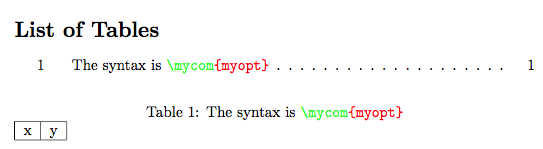
\includegraphics[width=0.8\columnwidth]{graphics/outputMWEdeclareRobustCommandCaptionElement.png}
\caption{Output of the MWE from Listing~\ref{lsting:MWEdeclareRobustCommandCaptionElement}}
\label{fig:MWEdeclareRobustCommandCaptionElement}
\end{jdrfigure}
\FloatBarrier
\subsection{Wrapping \lstinline|\\lstinline| within an \lstinline|\\mbox\{\}| can be useful}
\subsubsection{When a \lstinline|\\lstinline| is at the end of the line, you might need to wrap it within an \lstinline|\\mbox|}
\label{section:wrapEOLlstinlineInMbox}
Suppose you have a \lstinline|\lstinline| command that falls at the end of a typeset line, with more text in that paragraph awaiting to be typeset on the next line.

There are two situations in which this would create a typographical problem that you can solve through use of the \lstinline|\mbox| command:
\begin{jdr_itemize}
  \item \LaTeX{} creates an unwanted ``space'' at the beginning of the next line. See section~\ref{section:unwantedSpaceNextLine}.
  \item If that \lstinline|\lstinline| command is also the end of a sentence, and so is immediately followed by a period (.), \LaTeX{} can choose to typeset the period alone on the next line, separated from the last word of the sentence. See section~\ref{section:endingSentenceWithLstinlineRequireMbox}.
\end{jdr_itemize}

Both of these problems can be fixed by wrapping at least the \lstinline|\lstinline| command itself within an \lstinline|\mbox{}| command. Note, from the discussion in section~\ref{section:escapeCertainCharactersInsideArgument}, that any occurrences of \escapableCharactersJdrLst within the verbatim text of \lstinline|\lstinline| must be escaped because the \lstinline|\lstinline| command is within an argument of a command (viz., within the argument of \lstinline|\mbox{}|).

\paragraph{A \lstinline|\\lstinline| at the end of a typeset line can cause an unwanted space at the beginning of the next line}
\label{section:unwantedSpaceNextLine}
If you have a \lstinline|\lstinline| command that lands at the end of a typeset line, with more text for that paragraph awaiting typesetting on the next line, it might create an unwanted white space at the beginning of the next line. For example, while drafting this very document I encountered the typographical snafu shown in Figure~\ref{fig:snafuUnwantedWhitespaceBeginningOfALine} where there is an unwanted leading ``space'' before ``command'' on the third line, which is caused by the \mbox{\lstinline*\\lstinline|\\lstinline|*} command that winds up typeset as the last word on the previous line.
\begin{jdrfigure}[ht]
\centering
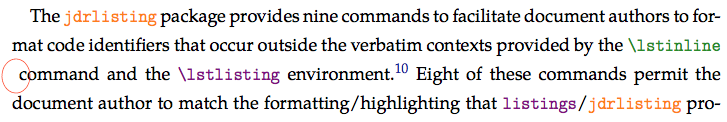
\includegraphics[width=0.8\columnwidth]{graphics/exampleUnwantedLeadingWhiteSpaceLstinlineEOL.png}
\caption{Unwanted whitespace at beginning of a line caused by a \lstinline|\\lstinline| command at the end of the previous line} 
\label{fig:snafuUnwantedWhitespaceBeginningOfALine}
\end{jdrfigure}

The \LaTeX{} code for the offending sentence is:
\begin{jdrCodeSnip}
%\label{codeeq:NAME}
\begin{lstlisting}
The \lstinline$jdrlisting$ package provides nine commands to facilitate document authors to format code identifiers that occur outside the verbatim contexts provided by the \lstinline$\lstinline$ command and the \lstinline$\lstlisting$ environment.
\end{lstlisting}
\end{jdrCodeSnip}

This extra-leading-space problem is solved by wrapping \lstinline|\lstinline$\lstinline$| within \lstinline|\mbox{}| like so:
\begin{jdrCodeSnip}
%\label{codeeq:NAME}
\lstinline|\mbox{\lstinline$\\lstinline$}|
\end{jdrCodeSnip}
where note that I escaped the backslash from the verbatim \lstinline|\lstinline| (i.e., the one wrapped in the \lstinline|$| delimiters) but not from the actual command \lstinline|\lstinline|. (This is an application of the escaping procedures discussed in greater detail in section~\ref{section:exampleEscapingCharactersWithinArgumentOfCommand}.)
\paragraph{If you end a sentence with a \lstinline|\\lstinline| snippet, you might need to wrap the snippet and its immediately following period inside an \lstinline|\\mbox|}
\label{section:endingSentenceWithLstinlineRequireMbox}

If a normal sentence ends with a word immediately followed by a period, \LaTeX{} will make sure that that period stays attached to the last letter of that last word. That last word may move to the next line, or may be hyphenated and its last syllable will move to the next line, but the period will definitely remain attached to the last letter. No way would \LaTeX{} send the period alone to the next line.

Not so if you have a sentence that ends with a \lstinline|\lstinline| command of verbatim code, which is then immediately followed by a period. \LaTeX{} doesn't necessarily keep the period glued to the \lstinline|\lstinline| command of verbatim code, and you can awkwardly have the period orphaned alone, beginning the next line.

If that happens, you can simply wrap both \jdrcircled{a}~the \lstinline|\lstinline| command of verbatim code and \jdrcircled{b}~the immediately following period all within an \lstinline|\mbox{}|. Do be aware that, because your \lstinline|\lstinline| command of verbatim code is now appearing within the argument of a command, viz., the \lstinline|\mbox|, you need to escape any occurrences of \escapableCharactersJdrLst.\footnote{See code snippet~\ref{codeeq:verbotenCharactersInVerbatimCodeInArguments} and section~\ref{section:escapeCertainCharactersInsideArgument}.}

For example, suppose you have a sentence that ends: ``after \lstinline|\begin{document}|.'' The corresponding \LaTeX{} code for this sentence fragment is:
\begin{jdrCodeSnip}
%\label{codeeq:NAME}
\lstinline*after \lstinline|\begin{document}|.*
\end{jdrCodeSnip}
Further suppose that, due to the particular length of the previous part of the paragraph, \LaTeX{} orphans the period alone on the next line.

To cure this, you'd wrap an \lstinline|\mbox{}| around both the \lstinline*\lstinline|\begin{document}|* and  the trailing period.

A first cut at this would look like:
\begin{jdrCodeSnip}
\label{codeeq:firstCutWrapMbox}
\lstinline*after \mbox{\lstinline|\begin{document}|.}*
\end{jdrCodeSnip}
However, this would fail because the \lstinline|\lstinline| expression \jdrcircled{a}~appears within the argument of a command (viz., \lstinline|\mbox|) and \jdrcircled{b}~the verbatim code includes verboten characters \lstinline|\|, \lstinline|{|, and \lstinline|}|. These verboten characters must be escaped from the verbatim code (and only from the verbatim code\footnote{To be clear, in code snippet~\ref{codeeq:firstCutWrapMbox}, there’s nothing objectionable about the \typewriterTeXCSColorJdrLstA{\textbackslash{}} in \lstinline|\\lstinline|. The only \typewriterTeXCSColorJdrLstA{\textbackslash{}} that needs escaping is the one in \lstinline|\\begin|.}) by prefixing each one with a \lstinline|\|. The correct syntax is:\footnote{This is an example of the same character-escaping technique explained in greater detail in section~\ref{section:exampleEscapingCharactersWithinArgumentOfCommand}.}
\begin{jdrCodeSnip}
%\label{codeeq:NAME}
\lstinline*after \mbox{\lstinline|\\begin\{document\}|.}*
\end{jdrCodeSnip}
\subsubsection{Wrapping a \lstinline|\\lstinline| command within an \lstinline|\\mbox\{\}| can ease using the same content in \jdrcircled{a}~body text as \jdrcircled{b}~in footnotes, captions, or sectioning commands}
While escaping \escapableCharactersJdrLst is necessary when the \lstinline|\lstinline| appears in the argument to another command, it is also the case, conversely, that one should \emph{not} escape these characters when the \lstinline|\lstinline| does not appear within an argument to another command: Unnecessary escaping would yield the incorrect result in which the escaping \descriptorStylejdrLst{\textbackslash{}}s were visible.

For example, if I wanted to display the string \escapableCharactersJdrLst, and I unnecessarily escaped each one, using the following:
\begin{jdrCodeSnip}
%\label{codeeq:NAME}
\lstinline*\lstinline|\{\}\#\%\\|*
\end{jdrCodeSnip}
the result would be: \lstinline|\{\}\#\%\\|, rather than \escapableCharactersJdrLst.

This ``feature''---that whether \escapableCharactersJdrLst should be escaped depends on whether the \lstinline|\lstinline| command appears in the argument of another command---is unfortunate.

As a specific example, it's common to decide at some point in drafting to relegate text in the body to a footnote or, conversely, to later decide to elevate the prominence of footnote text by moving it to the body. Ideally, the document author should be able freely to copy-and-paste text between \jdrcircled{a}~the body and \jdrcircled{b}~a footnote, caption, or sectioning command.

Instead---when the content includes a \lstinline|\lstinline| command that includes \escapableCharactersJdrLst---\jdrcircled{1}~moving from body text to a footnote, say, involves escaping these characters and, conversely, \jdrcircled{2}~moving from a footnote to body text requires \emph{un}escaping these characters.

To the extent that this poses a problem to the document author, one solution is to \jdrcircled{a}~wrap all such constructions (\lstinline|\lstinline| commands with \escapableCharactersJdrLst) in an \lstinline|\mbox{}| from the get-go and \jdrcircled{b}~escape all the \escapableCharactersJdrLst characters. Once wrapped inside an  \lstinline|\mbox{}|, these characters must be escaped regardless of whether the construction lies within body text or instead a footnote, caption, or sectioning command. Thus, the entire  \lstinline|\mbox{}| can be copied and pasted between these different contexts without changing the escaping of the \escapableCharactersJdrLst.


\subsection{Using \lstinline|\\lstinline| or \lstinline|lstlisting| to typeset code that itself includes \lstinline|\\lstinline| or \lstinline|lstlisting|, respectively, code}
The documentation you're reading this instant is an example of when you'd want to discuss code relating to the \lstinline|listings| package. This documentation uses the \lstinline|listings| package itself as the coding ``language'' to discuss itself, making the commands/environments of the \lstinline|listings| package an embedded metalanguage for this purpose.\footnote{See, for example, ``\href{https://en.wikipedia.org/wiki/Metalanguage#Embedded}{Types » Embedded}'' of ``\href{https://en.wikipedia.org/wiki/Metalanguage}{Metalanguage},'' Wikipedia, accessed October~2, 2018.}
\subsubsection{It's straightforward to use \lstinline|\\lstinline| to typeset code that includes \lstinline|\\lstinline| and any other \lstinline|listings| entities}
\label{section:nestedLstinlineIsEasy}
I discuss the syntax of the \lstinline|\lstinline| command in section~\ref{section:syntaxLstinline}:
\begin{jdrCodeSnip}
%\label{codeeq:NAME}
\lstinline[mathescape]|\lstinline[$\descriptorStylejdrLst{key=value list}$]$\descriptorStylejdrLst{<char>}\descriptorStylejdrLst{<verbatim code>}\descriptorStylejdrLst{<char>}$|
\end{jdrCodeSnip}
where \descriptorStylejdrLst{<char>} refers to a single character that is not found in \descriptorStylejdrLst{<verbatim code>}.\footnote{It's better to avoid using an opening square bracket (i.e., \lstinline|[|) as the delimiter because \lstinline$\\lstinline$ has to scan for that character because it would delimit the command's optional argument. See ListingsDocs at~§~4.2. (``Since the command first looks ahead for an optional argument, you must provide at least an empty one if you want to use \lstinline$[$ as \emph{<character>}.'')} This single character both immediately precedes and immediately follows the string of code to be rendered verbatim.\footnote{This convention, which leaves the delimiter undesignated ex ante, allows the delimiter to be chosen according to the string desired to be rendered verbatim.}

In effect, once \LaTeX{} determines \descriptorStylejdrLst{<char>} by encountering it, \LaTeX{} stops interpreting the subsequent characters as meeaningful \LaTeX{} code until it encounters \descriptorStylejdrLst{<char>} a second time.

As a result, there is no problem with the \lstinline|\lstinline| command referencing itself, even deeply nested; this just requires changing the delimiting character for each level of reference:
\begin{jdrCodeSnip}
\label{codeeq:deeplyNestedLstinline}
\lstinline*\lstinline|\lstinline|*\\
\lstinline^\lstinline*\lstinline|\lstinline|*^\\
\lstinline@\lstinline^\lstinline*\lstinline|\lstinline|*^@\\
\end{jdrCodeSnip}
The output of code snippet~\ref{codeeq:deeplyNestedLstinline} is:
\begin{quote}
\lstinline|\lstinline|\\
\lstinline*\lstinline|\lstinline|*\\
\lstinline^\lstinline*\lstinline|\lstinline|*^\\
\end{quote}
\subsubsection{Choosing an environment to enclose code that includes \mbox{\lstinline|\\begin\{lstlisting\}|} and \mbox{\lstinline|\\end\{lstlisting\}|}}
\paragraph{The \lstinline|lstlisting| environment cannot be nested because a verbatim \mbox{\lstinline|\\end\{lstlisting\}|} will cause early termination}
\label{section:lstlistingEnvironmentsCannotBeNested}
Although it's simple for the \lstinline|\lstinline| command to reference itself, because of its flexibly chosen delimiter character,\footnote{ See section~\ref{section:nestedLstinlineIsEasy}.} the same cannot be said for the \lstinline|lstlisting| environment because its beginning and ending statements---\lstinline|\begin{lstlisting}| and \mbox{\lstinline|\\end\{lstlisting\}|}, respectively---are fixed.

Consider the following attempt to nest the \lstinline|lstlisting| environment:

\begin{jdrCodeSnip}
\label{codeeq:attemptNestLstlisting}
\lstinline|\begin{lstlisting}|\\
\lstinline|\begin{lstlisting}|\\
\lstinline|% Here's some code|\\
\lstinline|\end{lstlisting}|\\
\lstinline|\end{lstlisting}|\\
\end{jdrCodeSnip}

The desired output from code snippet~\ref{codeeq:attemptNestLstlisting} would be:
\begin{jdrCodeSnip}
\label{codeeq:idealOutputNestedLstlisting}
\lstinline|\begin{lstlisting}|\\
\lstinline|% Here's some code|\\
\lstinline|\end{lstlisting}|\\
\end{jdrCodeSnip}

However, the actual output from code snippet~\ref{codeeq:attemptNestLstlisting} is:
\begin{jdrCodeSnip}
%\label{codeeq:NAME}
\lstinline|\begin{lstlisting}|\\
\lstinline|% Here's some code|\\
\end{jdrCodeSnip}
In other words, the output is cutoff prematurely---leaving \lstinline|\end{lstlisting}| untypeset. This early termination occurs because the first time \lstinline|\end{lstlisting}| is encountered, it is interpreted not as being part of the verbatim code to typeset but rather as the termination of the original \lstinline|lstlisting| environment.\footnote{This is also explained in \href{https://tex.stackexchange.com/a/31981/7922}{Peter Grill's answer} to ``\href{https://tex.stackexchange.com/questions/31980/masking-endlstlisting}{Masking \lstinline|\\end\{lstlisting\}|},'' \TeX Stack Exchange, October~18, 2011. (``I don't think you can nest within the \lstinline|lstlisting| environment. Since this is a verbatim environment, the second \mbox{\lstinline|\\begin\{lstlisting\}|} is ignored, and the first \mbox{\lstinline|\\end\{lstlisting\}|} results in the termination of the outer \mbox{\lstinline|\\begin\{lstlisting\}|} leaving an extra \mbox{\lstinline|\\end\{lstlisting\}|}.'')}\footnote{Werner offers a workaround, using \lstinline|[mathescape]| and a string \lstinline|$$| between the \lstinline|\\| and \lstinline|end\{lstlisting\}| of the verbatim \lstinline|\\end\{lstlisting\}|, in \href{https://tex.stackexchange.com/a/31986/7922}{his answer} to ``\href{https://tex.stackexchange.com/questions/31980/masking-endlstlisting}{Masking \lstinline|\\end\{lstlisting\}|},'' \TeX Stack Exchange, October~18, 2011.}

\paragraph{The \lstinline|jdrLstListing| environment from the \lstinline|jdrlisting| package can wrap a verbatim \lstinline|lstlisting| environment}
\label{section:jdrLstListingCanWrapLstListing}
In section~\ref{section:lstlistingEnvironmentsCannotBeNested}, I showed that you can't nest \lstinline|lstlisting| environments because a verbatim instance of \lstinline|\end{lstlisting}| is confused for being an actual instance of \mbox{\lstinline|\\end\{lstlisting\}|}, causing the environment to terminate prematurely and incompletely.

The \lstinline|jdrlisting| package defines a new environment, \lstinline|jdrLstListing|, to get around this problem.\footnote{This is suggested by \href{https://tex.stackexchange.com/a/31984/7922}{Enrico Gregorio's answer} to ``\href{https://tex.stackexchange.com/questions/31980/masking-endlstlisting}{Masking \lstinline|\\end\{lstlisting\}|},'' \TeX Stack Exchange, October~18, 2011. (``If you want to show examples of \lstinline|lstlisting| itself, define a different environment [using \lstinline|\\lstnewenvironment|]\ldots.'')}

The \lstinline|jdrLstListing| environment is nothing other than the \lstinline|lstlisting| environment itself but with a different name. By invoking the \lstinline|jdrLstListing| environment with \mbox{\lstinline|\\begin\{jdrLstListing\}|}, \LaTeX{} will continue to treat all following text as verbatim, rather than meaningful \LaTeX{} code, until an \mbox{\lstinline|\\end\{jdrLstListing\}|} is encountered. Thus, encountering a verbatim \mbox{\lstinline|\\end\{lstlisting\}|} will not cause the \lstinline|jdrLstListing| environment environment to prematurely terminate.

We can transform the failed attempt to nest \lstinline|lstlisting| environments, code snippet~\ref{codeeq:attemptNestLstlisting}, by replacing the outer (actual, non-verbatim) \lstinline|lstlisting| environment with an equivalent but differently named \lstinline|jdrLstListing| environment:

\begin{jdrCodeSnip}
\label{codeeq:wrapLstlistingInJdrLstListing}
\lstinline|\begin{jdrLstListing}|\\
\lstinline|\begin{lstlisting}|\\
\lstinline|% Here's some code|\\
\lstinline|\end{lstlisting}|\\
\lstinline|\end{jdrLstListing}|\\
\end{jdrCodeSnip}

These reformed quasi-nested environments does indeed yield the desired output code snippet~\ref{codeeq:idealOutputNestedLstlisting}.

That said\ldots although the \lstinline|jdrLstListing| environment \emph{theoretically} solves the problem (that \lstinline|lstlisting| environments can't be nested), in practice the ceasefire appears fragile.\footnote{I’ve often had the experience where the incremental addition of additional verbatim code inexplicably breaks something and compilation fails. It has been impossible to track down through conventional divide-and-conquer methods what the problem is.}

\paragraph{The \lstinline|LTXexample| environment from the \lstinline|showexpl| package is a verbatim alternative that simultaneously displays the output of the code}
\href{https://ctan.org/pkg/showexpl?lang=en}{Rolf Niepraschk's \lstinline|showexpl| package} provides the \lstinline|LTXexample| environment ``to typeset \LaTeX{} source code and the related result in the same document.''\footnote{For documentation, see Rolf Niepraschk, ``\href{http://mirrors.ctan.org/macros/latex/contrib/showexpl/doc/showexpl.pdf}{The \lstinline|showexpl| package},'' December~11, 2016. In addition, the author provides a \href{https://github.com/rolfn/showexpl}{GitHub repository} and a document of examples as \href{http://mirrors.ctan.org/macros/latex/contrib/showexpl/doc/showexpl-test.pdf}{pdf} and its \href{https://github.com/rolfn/showexpl/blob/master/doc/showexpl-test.tex}{source on GitHub}.}

The syntax of the \lstinline|LTXexample| environment is:\footnote{Rolf Niepraschk, ``\href{http://mirrors.ctan.org/macros/latex/contrib/showexpl/doc/showexpl.pdf}{The \lstinline|showexpl| package},'' December~11, 2016, on pages~1–2.}
\begin{jdrCodeSnip}
%\label{codeeq:NAME}
\lstinline[mathescape]|\begin{LTXexample}[$\descriptorStylejdrLst{key=value list}$]|\\
\lstinline$%   Some code$\\
\lstinline$\end{LTXexample}$
\end{jdrCodeSnip}
where the \descriptorStylejdrLst{key=value list} allows the specification of any of more than a dozen parameters.\footnote{See Rolf Niepraschk, ``\href{http://mirrors.ctan.org/macros/latex/contrib/showexpl/doc/showexpl.pdf}{The \lstinline|showexpl| package},'' December~11, 2016, pages~1–2, for details. The document of examples (as \href{http://mirrors.ctan.org/macros/latex/contrib/showexpl/doc/showexpl-test.pdf}{pdf} and its \href{https://github.com/rolfn/showexpl/blob/master/doc/showexpl-test.tex}{source on GitHub}) has illustrations to illucidate the meanings of some of these parameters.} In particular, you can choose whether you want the output presented to the left, to the right, above, or below the source code.\footnote{As far as I can tell, there is no option to suppress the output entirely.}

\section{Commands to emulate or extend \lstinline|listings| syntax highlighting in text outside of \lstinline|\\lstinline| or \lstinline|lstlisting|-type environments}
\label{section:emulationCommands}
Use of this package, \lstinline|jdrlisting|, results in identifiers in listings being formatted according to the identifier's category (and class).

There are use cases in which a document author will want to be able to apply the same formatting to a term when it's not in a listing (i.e., neither an argument to \lstinline|\lstinline| nor enclosed in a \lstinline|lstlisting| environment).\footnote{[[This section would be strengthened by including examples, which could be drawn from elsewhere in this same document.]]}

The commands listed in Table~\ref{table:listEmulationCommandsDiscussionLocations} and discussed below facilitate that. 

\begin{jdrtable}[!htb] % p option positions table on its own page.
%\rowcolors{2}{tableShade}{jdrTableBackgroundColor}  % start alternating shades from 2nd row (not counting header)
\centering
\caption{Commands provided by the \lstinline|jdrlisting| package to emulate or extend \lstinline|listings| syntax highlighting in text outside of \lstinline|\\lstinline| or \lstinline|lstlisting|-type environments, and where they are discussed in this document}
\label{table:listEmulationCommandsDiscussionLocations}
\begin{tabular}[t]{p{6.95cm}K{1.25cm}p{6.25cm}}
%\toprule
Command & § & Comment \\
\midrule
\lstinline|\typewriterBasicColorJdrLst| & \ref{section:emulateBasicStyle} & Emulate \lstinline|basicstyle| \\
\lstinline|\typewriterIdentifierColorJdrLst| & \ref{section:emulateIdentifierStyle} & Emulate \lstinline|identifierstyle| \\
\lstinline|\typewriterKeywordColorJdrLst| & \ref{section:emulateKeywordStyle} & Emulate \lstinline|keywordstyle| \\
\midrule
\lstinline|\typewriterEmphColorJdrLstA| & \ref{section:emulateEmphStyle} & Emulate Class~\#1 of \lstinline|emphstyle| \\
\lstinline|\typewriterEmphColorJdrLstB| & \ref{section:emulateEmphStyle} & Emulate Class~\#2 of \lstinline|emphstyle| \\
\midrule
\lstinline|\typewriterTeXCSColorJdrLstA| & \ref{section:emulateTeXcsStyle} & Emulate Class~\#1 of \lstinline|texcsstyle| \\
\lstinline|\typewriterTeXCSColorJdrLstB| & \ref{section:emulateTeXcsStyle} & Emulate Class~\#2 of \lstinline|texcsstyle| \\
\lstinline|\typewriterTeXCSColorJdrLstC| & \ref{section:emulateTeXcsStyle} & Emulate Class~\#3 of \lstinline|texcsstyle| \\
\midrule
\lstinline|\descriptorStylejdrLst| & \ref{section:emulateMetaDescriptor} & Format meta descriptors \\
%\bottomrule
\end{tabular}
\end{jdrtable}%

\subsection{\lstinline|\\typewriterBasicColorJdrLst| to emulate \lstinline|basicstyle|}
\label{section:emulateBasicStyle}
The command \lstinline|\typewriterBasicColorJdrLst| emulates the \lstinline|basicstyle| format. Its syntax is:
\begin{jdrCodeSnip}
%\label{codeeq:NAME}
\lstinline[mathescape]|\typewriterBasicColorJdrLst{$\descriptorStylejdrLst{term}$}|
\end{jdrCodeSnip}

\subsection{\lstinline|\\typewriterIdentifierColorJdrLst| to emulate \lstinline|identifierstyle|}
\label{section:emulateIdentifierStyle}
The command \lstinline|\typewriterIdentifierColorJdrLst| emulates the \lstinline|identifierstyle| format. Its syntax is:
\begin{jdrCodeSnip}
%\label{codeeq:NAME}
\lstinline[mathescape]|\typewriterIdentifierColorJdrLst{$\descriptorStylejdrLst{term}$}|
\end{jdrCodeSnip}

\subsection{\lstinline|\\typewriterKeywordColorJdrLst| to emulate \lstinline|keywordstyle|}
\label{section:emulateKeywordStyle}
The command \lstinline|\typewriterKeywordColorJdrLst| emulates the \lstinline|keywordstyle| format. Its syntax is:
\begin{jdrCodeSnip}
%\label{codeeq:NAME}
\lstinline[mathescape]|\typewriterKeywordColorJdrLst{$\descriptorStylejdrLst{term}$}|
\end{jdrCodeSnip}

\subsection{\lstinline|\\emphColorTypewriterjdrLst|\textcolor{colorDescriptorJdrLst}{$\alpha$} commands to emulate the classes of \lstinline|emphstyle|}
\label{section:emulateEmphStyle}
There are two commands of the form \mbox{\lstinline|\\emphColorTypewriterjdrLst|\textcolor{colorDescriptorJdrLst}{$\alpha$},} for $\alpha=$ \lstinline|A| and~\lstinline|B|, that emulate Classes~\#1 and~\#2, respectively, of the \lstinline$emphstyle$.

The command \lstinline|\typewriterEmphColorJdrLstA| emulates class~\#1 of the \lstinline|emphstyle| format. Its syntax is:
\begin{jdrCodeSnip}
%\label{codeeq:NAME}
\lstinline[mathescape]|\typewriterEmphColorJdrLstA{$\descriptorStylejdrLst{term}$}|
\end{jdrCodeSnip}

The command \lstinline|\typewriterEmphColorJdrLstB| emulates class~\#2 of the \lstinline|emphstyle| format. Its syntax is:
\begin{jdrCodeSnip}
%\label{codeeq:NAME}
\lstinline[mathescape]|\typewriterEmphColorJdrLstB{$\descriptorStylejdrLst{term}$}|
\end{jdrCodeSnip}

\subsection{\lstinline|\\TeXCSColorTypewriterjdrLst|\textcolor{colorDescriptorJdrLst}{$\alpha$} commands to emulate the classes of \lstinline|texcsstyle|}
\label{section:emulateTeXcsStyle}
There are two commands of the form \mbox{\lstinline|\\TeXCSColorTypewriterjdrLst|\textcolor{colorDescriptorJdrLst}{$\alpha$},} for $\alpha=$ \lstinline|A|, \lstinline$B$, and~\lstinline|C|, that emulate Classes~\#1, \#2, and~\#3, respectively, of the \lstinline$texcsstyle$.

The command \lstinline|\typewriterTeXCSColorJdrLstA| emulates class~\#1 of the \lstinline|texcsstyle| format. Its syntax is:
\begin{jdrCodeSnip}
%\label{codeeq:NAME}
\lstinline[mathescape]|\typewriterTeXCSColorJdrLstA{$\descriptorStylejdrLst{term}$}|
\end{jdrCodeSnip}

The command \lstinline|\typewriterTeXCSColorJdrLstB| emulates class~\#2 of the \lstinline|texcsstyle| format. Its syntax is:
\begin{jdrCodeSnip}
%\label{codeeq:NAME}
\lstinline[mathescape]|\typewriterTeXCSColorJdrLstB{$\descriptorStylejdrLst{term}$}|
\end{jdrCodeSnip}

The command \lstinline|\typewriterTeXCSColorJdrLstC| emulates class~\#3 of the \lstinline|texcsstyle| format. Its syntax is:
\begin{jdrCodeSnip}
%\label{codeeq:NAME}
\lstinline[mathescape]|\typewriterTeXCSColorJdrLstC{$\descriptorStylejdrLst{term}$}|
\end{jdrCodeSnip}

\subsection{\lstinline|\\descriptorStylejdrLst| to format meta descriptors}
\label{section:emulateMetaDescriptor}
\subsubsection{A meta descriptor can explain what an argument is expecting}
It's best to start this discussion with an example. Suppose we want to discuss the syntax of a command \lstinline|\jdrHlineTC|, which takes two arguments. Part of the syntax is specifying what kinds of constant or variable should be put into each of the arguments. We could describe this syntax as:
\begin{jdrCodeSnip}
\label{codeeq:exampleDescriptor}
\lstinline[mathescape]|\jdrHlineTC{$\descriptorStylejdrLst{length}$}{$\descriptorStylejdrLst{color}$}|
\end{jdrCodeSnip}
In code snippet~\ref{codeeq:exampleDescriptor}, \descriptorStylejdrLst{length} and \descriptorStylejdrLst{color} are what I will call \emph{descriptors}. Each appears between curly braces where an argument would appear in actual code.

The \emph{descriptor} is a category of word or phrase that \jdrcircled{a}~you would embed within a code snippet but \jdrcircled{b}~is not literally code itself---you wouldn't actually find it in code; it might be quite syntactically incorrect if you did. Moreover, a descriptor is not a type of identifier that is recognized by the \lstinline$listings$ package.

A descriptor is \emph{metacode}: it is useful for \emph{talking about code}. In particular, the descriptor's purpose is to indicate to the reader what type of code entity should be inserted in lieu of the descriptor and what that code entity's interpretation is.

You'd never literally write \lstinline$length$ where \descriptorStylejdrLst{length} appears. Instead, you'd supply a valid expression for a length, e.g., \lstinline$10pt$ or \lstinline$\arrayrulewidth$. Likewise, you'd never write \lstinline$color$ where {\descriptorStylejdrLst{color}} appears; you'd instead supply a defined name that refers to a valid color, e.g., \lstinline$MidnightBlue$.
\subsubsection{The \lstinline|\\descriptorStylejdrLst| command applies descriptor-specific formatting to its argument}
Because a descriptor is not typically found in code, it is less likely that \jdrcircled{a}~you'd want to typeset a descriptor in a \lstinline$lstlisting$ environment than that \jdrcircled{b}~you'd want to typeset a descriptor in inline code using \lstinline$\lstinline$. 

Because descriptors are not recognized by the \lstinline$listings$ package as a known type of snippet, that package does not automatically specially format descriptors.

To allow for appropriate syntax highlighting for descriptors, the \lstinline$jdrlisting$ package defines a command, \lstinline$\descriptorStylejdrLst$, that applies the desired formatting to its argument. This command is defined to be:
\begin{jdrCodeSnip}
\label{codeeq:definitiondescriptorStylejdrLst}
\lstinline|\newcommand{\descriptorStylejdrLst}[1]%|\\
\lstinline|     {\textcolor{jdrDescriptorColor}{\textrm{\textit{#1}}}}|
\end{jdrCodeSnip}
i.e., it sets the type to \jdrcircled{a}~a serif font that \jdrcircled{b}~is italicized and \jdrcircled{c}~\textcolor{colorDescriptorJdrLst}{colored as colorDescriptorJdrLst}, e.g., \descriptorStylejdrLst{some descriptor}.
\subsubsection{Using \lstinline|\\descriptorStylejdrLst| within \lstinline|\\lstinline| requires the optional \mbox{\lstinline|[mathescape]|} key in order to ``escape to \LaTeX''}
\label{section:usingMathescapeWithinLstinline}
In code snippet~\ref{codeeq:exampleDescriptor}, the descriptor portions (viz., \descriptorStylejdrLst{length} and \descriptorStylejdrLst{color}) appear embedded within verbatim code formatted by \lstinline|\lstinline|.

To accomplish that we need to tell \lstinline|\lstinline| to pause its verbatim approach to its argument and instead, temporarily, interpret \lstinline|\descriptorStylejdrLst{length}| and \lstinline|\descriptorStylejdrLst{color}| as actual \LaTeX{} instructions to process. This is called ``escaping to \LaTeX{}.'' To do this, we use the optional key \lstinline|[mathescape]| when we call \lstinline|\lstinline|.\footnote{See ListingsDocs, §~4.14 (``Escaping to \LaTeX’’).} \lstinline|mathescape|, when present or \lstinline|true|, ``activates… special behavior of the dollar sign. If activated a dollar sign acts at \TeX's text math shift.''

Using this capability, code snippet~\ref{codeeq:exampleDescriptor} is achieved by the following \lstinline|\lstinline| command:
\begin{jdrCodeSnip}
%\label{codeeq:mathescapeCodeForExample}
\lstinline*\lstinline[mathescape]|%*\\
\lstinline*    \jdrHlineTC{$\descriptorStylejdrLst{length}$}%*\\
\lstinline*    {$\descriptorStylejdrLst{color}$}|*
\end{jdrCodeSnip}

\subsubsection{Using math mode within \lstinline|\\descriptorStylejdrLst| to achieve, e.g., \descriptorStylejdrLst{$n_{args}$}, in conjunction with \lstinline|\\lstinline[mathescape]|}
\label{section:usingMathescapeWithinLstinlineMathmode}
You might want to use \lstinline|\descriptorStylejdrLst| to produce a descriptor that is truly a math-mode expression, e.g., \descriptorStylejdrLst{$n_{args}$}.\footnote{See, for example, code snippet~\ref{codeeq:lstnewenvironmentSyntax} in section~\ref{section:lstnewenvironmentSyntax}.}

If you are using \lstinline|\descriptorStylejdrLst| outside of the \lstinline|\lstinline[mathescape]| context, this is accomplished as simply as wrapping the desired math-mode expression between \mbox{\lstinline|$|\ldots\lstinline|$|}:
\begin{jdrCodeSnip}
%\label{codeeq:NAME}
\lstinline|\descriptorStylejdrLst{$n_{args}$}|
\end{jdrCodeSnip}

However, \emph{inside} the \lstinline|\lstinline[mathescape]| context, this attempt, i.e.,
\begin{jdrCodeSnip}
%\label{codeeq:NAME}
\lstinline*\lstinline[mathescape]|$\descriptorStylejdrLst{$n_{args}$}$|*
\end{jdrCodeSnip}
fails because the opening \lstinline|$| of \lstinline|$n_{args}$| is perceived to be the closing \lstinline|$| of \mbox{\lstinline*\\lstinline[mathescape]$*.}

The workaround is to ``hide'' the \lstinline|$|s of \lstinline|$n_{args}$| by first defining a command:
\begin{jdrCodeSnip}
%\label{codeeq:NAME}
\lstinline|\newcommand{\nArgs}{$n_{args}$}|
\end{jdrCodeSnip}
and then insert \lstinline|\nArgs| into the argument of \lstinline|\descriptorStylejdrLst|:
\begin{jdrCodeSnip}
%\label{codeeq:NAME}
\lstinline*\lstinline[mathescape]|$\descriptorStylejdrLst{\nArgs}$|*
\end{jdrCodeSnip}

The workaround is incomplete, however. I haven't found a way to achieve \descriptorStylejdrLst{$n_{args}$} where the ``args'' appears as non--math mode text, i.e., as \mbox{$n_\text{args}$}. And this is true even outside the \lstinline*\lstinline[mathescape]* context. For example, in \mbox{\lstinline|\\descriptorStylejdrLst\{$n_\\text\{args\}$\}|}, the \lstinline|\text{}| is apparently ignored or overridden; this renders as \mbox{\descriptorStylejdrLst{$n_\text{args}$}}.

\section{Specially emphasizing the identifiers from a particular package when writing documentation about that package}
\label{section:specialEmphasisParticularPackage}
Section~\ref{section:schemeLaTeXCategoryClasses} lays out the scheme I have chosen that specifies how:
\begin{jdr_itemize}
  \item \TeX{} control sequences are divided between three classes of \lstinline|texcs| identifiers:
    \begin{jdr_itemize}
    \item Class \#1: \TeX{} control sequences in the \lstinline$listings$ definition of \LaTeX{}
    \item Class \#2: \TeX{} control sequences harvested from third-party packages (including, by default, my own packages)
    \item Class \#3: \TeX{} control sequences of particular document-specific significance
\end{jdr_itemize}
  \item identifiers---excluding \TeX{} control sequences---such as names of packages, environments, keys, and values are divided between two classes of \lstinline|emph| identifiers
    \begin{jdr_itemize}
    \item Class~\#1: Names of packages, environments, keys, and values from standard \LaTeX{} or third-party packages, including by default my own packages
    \item Class~\#2: Names of packages, environments, keys, and values from packages of particular significance to the specific document
\end{jdr_itemize}
\end{jdr_itemize}

In other words, by default the document-specific classes of both types of identifiers, viz., \jdrcircled{a}~Class~\#3 of the \lstinline|texcs| identifiers and \jdrcircled{b}~Class~\#2 of the \lstinline|emph| identifiers, are empty. By default, all identifiers from third-party packages reside either in \jdrcircled{a}~Class~\#2 of \lstinline|texcs| identifiers or \jdrcircled{b}~Class~\#1 of \lstinline|emph| identifiers.

In order to have the identifiers associated with a particular package be specially highlighted to make them distinctly highlighted from identifiers from standard \LaTeX{} or other third-party packages, the document author must:
\begin{jdr_itemize}
  \item promote the \TeX{} control sequences of the distinguished package from Class~\#2 to Class~\#3 of \lstinline|texcs| identifiers, and
  \item promote the \lstinline|emph| identifiers of the distinguished package from Class~\#1 to Class~\#2 of \lstinline|emph| identifiers.
\end{jdr_itemize}

This \lstinline|jdrlisting| package provides a set of commands such that a document author can specially highlight both types of identifiers for a given package by issuing a single command.

These commands are of the form \typewriterTeXCSColorJdrLstC{\textbackslash{}emphasizeIdentifiers$x$}, where \typewriterTeXCSColorJdrLstC{$x$} identifies the particular package. For example, when \mbox{{\color{colorTeXCSStyleJdrLstC}${x}=$}\typewriterTeXCSColorJdrLstC{JdrArticle}}, the command is \lstinline|\emphasizeIdentifiersJdrArticle|, which emphasizes the identifiers for the \lstinline|jdrarticle| package.

These commands are listed and described in Table~\ref{table:listJDRPackageEmphasisCommandsDiscussionLocations}.

\begin{jdrtable}[!htb] % p option positions table on its own page.
%\rowcolors{2}{tableShade}{jdrTableBackgroundColor}  % start alternating shades from 2nd row (not counting header)
\centering
\caption{Commands provided by the \lstinline|jdrlisting| package to emphasize/unemphasize the identifiers of particular JDR packages, and where they are discussed in this document}
\label{table:listJDRPackageEmphasisCommandsDiscussionLocations}
\begin{tabular}[t]{p{7.17cm}p{7.5cm}}
%\toprule
Command & Description \\
\midrule
\lstinline|\emphasizeIdentifiersJdrListing|     & Emphasize identifiers from the \lstinline|jdrlisting| package \\
\lstinline|\unemphasizeIdentifiersJdrListing|   & Unemphasize identifiers from the \lstinline|jdrlisting| package \\
\lstinline|\emphasizeIdentifiersJdrSgame|       & Emphasize identifiers from the \lstinline|jdrsgame| package \\
\lstinline|\unemphasizeIdentifiersJdrSgame|     & Unemphasize identifiers from the \lstinline|jdrsgame| package \\
\lstinline|\emphasizeIdentifiersJdrUnicode|     & Emphasize identifiers from the \lstinline|jdrunicode| package \\
\lstinline|\unemphasizeIdentifiersJdrUnicode|   & Unemphasize identifiers from the \lstinline|jdrunicode| package \\
\lstinline|\emphasizeIdentifiersJdrArticle|     & Emphasize identifiers from the \lstinline|jdrarticle| package \\
\lstinline|\unemphasizeIdentifiersJdrArticle|   & Unemphasize identifiers from the \lstinline|jdrarticle| package \\
\lstinline|\emphasizeIdentifiersJdrHcline|      & Emphasize identifiers from the \lstinline|jdrhcline| package \\
\lstinline|\unemphasizeIdentifiersJdrHcline|    & Unemphasize identifiers from the \lstinline|jdrhcline| package \\
%\bottomrule
\end{tabular}
\end{jdrtable}%

\FloatBarrier



\section{My scheme of identifier-category classes and what identifiers to assign to each of them}
\label{section:schemeLaTeXCategoryClasses}
The remainder of this documentation assumes that you're familiar with the discussion of the \lstinline|listings| package in section~\ref{section:reviewListingsPackage}.

The \lstinline$jdrlisting$ package embodies my personalized scheme for syntax highlighting \LaTeX{} code in conjunction with the \lstinline|listings| package. The most fundamental characteristics of that scheme are how to group identifiers and how, on that basis, to format them. Table~\ref{table:mySchemeLaTeXCategoryClassesWhatAndColors} details my scheme.

\subsection{\TeX{} control sequences}
\label{section:schemeLaTeXtexcs}
I implement three classes of the \lstinline$texcs$ identifier category. See section~\ref{section:texcsClassA}, section~\ref{section:texcsClassB}, and section~\ref{section:texcsClassC}, respectively.

Each of the three classes receives a color with a name of the form \mbox{\lstinline|jdrLstColorTeXCSStyle|\descriptorAlpha}, where \descriptorAlpha is \lstinline$A$, \lstinline$B$, or \lstinline$C$, respectively.

\subsubsection{Class \#1: \TeX{} control sequences in the \lstinline$listings$ definition of \LaTeX{}}
\label{section:texcsClassA}
The first class is for those \TeX{} control sequences that are part of the definition within \lstinline$listings$ of the \LaTeX{} dialect of the \TeX{} language.\footnote{See \biblioForLanguageDefinitions.}

Implementing this class \emph{should} require no effort on the part of the \lstinline$jdrlisting$ package, because it should be preconfigured by the \lstinline$listings$ package. However, some standard-\LaTeX{} control sequences are defined in the language specification in such a way that they are not actually recognized as \lstinline|texcs|;\footnote{These control sequences \emph{are} declared as values for the \lstinline|moretexcs| key, but in a command \lstinline|\\lst@definelanguage[AlLaTeX]\{TeX\}[LaTeX]\{TeX\}|; whereas the other, effective, \lstinline|texcs| declarations are in a command \lstinline|\\lst@definelanguage[LaTeX]\{TeX\}[common]\{TeX\}|.} I refer to these as omitted \TeX{} control sequences. I added a subset of these omitted \TeX{} control sequences to a definition in \lstinline|jdrlisting| that assigns them to this first class of \lstinline|texcs| identifiers.\footnote{The subset is added to the definition of the command \lstinline|\\moreTeXcsOmittedStandardLaTeX|.}\footnote{The following is a list of the omitted \TeX{} control sequences; the subset that I manually added to the first class are the control sequences (\textcolor{colorTeXCSStyleJdrLstA}{that are colored like this}): \mbox{\lstinline|\\AtBeginDocument|,} \mbox{\lstinline|\\AtBeginDvi|,} \mbox{\lstinline|\\AtEndDocument|,} \mbox{\lstinline|\\AtEndOfClass|,} \mbox{\lstinline|\\AtEndOfPackage|,} \mbox{\lstinline|\\ClassError|,} \mbox{\lstinline|\\ClassInfo|,} \mbox{\lstinline|\\ClassWarning|,} \mbox{\lstinline|\\ClassWarningNoLine|,} \mbox{\lstinline|\\CurrentOption|,} \mbox{\lstinline|\\DeclareErrorFont|,} \mbox{\lstinline|\\DeclareFixedFont|,} \mbox{\lstinline|\\DeclareFontEncoding|,} \mbox{\lstinline|\\DeclareFontEncodingDefaults|,} \mbox{\lstinline|\\DeclareFontFamily|,} \mbox{\lstinline|\\DeclareFontShape|,} \mbox{\lstinline|\\DeclareFontSubstitution|,} \mbox{\lstinline|\\DeclareMathAccent|,} \mbox{\lstinline|\\DeclareMathAlphabet|,} \mbox{\lstinline|\\DeclareMathAlphabet|,} \mbox{\lstinline|\\DeclareMathDelimiter|,} \mbox{\lstinline|\\DeclareMathRadical|,} \mbox{\lstinline|\\DeclareMathSizes|,} \mbox{\lstinline|\\DeclareMathSymbol|,} \mbox{\lstinline|\\DeclareMathVersion|,} \mbox{\lstinline|\\DeclareOldFontCommand|,} \mbox{\lstinline|\\DeclareOption|,} \mbox{\lstinline|\\DeclarePreloadSizes|,} \mbox{\lstinline|\\DeclareRobustCommand|,} \mbox{\lstinline|\\DeclareSizeFunction|,} \mbox{\lstinline|\\DeclareSymbolFont|,} \mbox{\lstinline|\\DeclareSymbolFontAlphabet|,} \mbox{\lstinline|\\DeclareTextAccent|,} \mbox{\lstinline|\\DeclareTextAccentDefault|,} \mbox{\lstinline|\\DeclareTextCommand|,} \mbox{\lstinline|\\DeclareTextCommandDefault|,} \mbox{\lstinline|\\DeclareTextComposite|,} \mbox{\lstinline|\\DeclareTextCompositeCommand|,} \mbox{\lstinline|\\DeclareTextFontCommand|,} \mbox{\lstinline|\\DeclareTextSymbol|,} \mbox{\lstinline|\\DeclareTextSymbolDefault|,} \mbox{\lstinline|\\ExecuteOptions|,} \mbox{\lstinline|\\GenericError|,} \mbox{\lstinline|\\GenericInfo|,} \mbox{\lstinline|\\GenericWarning|,} \mbox{\lstinline|\\IfFileExists|,} \mbox{\lstinline|\\InputIfFileExists|,} \mbox{\lstinline|\\LoadClass|,} \mbox{\lstinline|\\LoadClassWithOptions|,} \mbox{\lstinline|\\MessageBreak|,} \mbox{\lstinline|\\OptionNotUsed|,} \mbox{\lstinline|\\PackageError|,} \mbox{\lstinline|\\PackageInfo|,} \mbox{\lstinline|\\PackageWarning|,} \mbox{\lstinline|\\PackageWarningNoLine|,} \mbox{\lstinline|\\PassOptionsToClass|,} \mbox{\lstinline|\\PassOptionsToPackage|,} \mbox{\lstinline|\\ProcessOptionsProvidesClass|,} \mbox{\lstinline|\\ProvidesFile|,} \mbox{\lstinline|\\ProvidesFile|,} \mbox{\lstinline|\\ProvidesPackage|,} \mbox{\lstinline|\\ProvideTextCommand|,} \mbox{\lstinline|\\RequirePackage|,} \mbox{\lstinline|\\RequirePackageWithOptions|,} \mbox{\lstinline|\\SetMathAlphabet|,} \mbox{\lstinline|\\SetSymbolFont|,} \mbox{\lstinline|\\TextSymbolUnavailable|,} \mbox{\lstinline|\\UseTextAccent|,} \mbox{\lstinline|\\UseTextSymbol|}.)}

This class of language/dialect--defined \TeX{} control sequences receives the color named \lstinline$colorTeXCSStyleJdrLstA$.

\subsubsection{Class \#2: \TeX{} control sequences harvested from third-party packages}
\label{section:texcsClassB}
The second class is additional \TeX{} control sequences that I have harvested from third-party packages and manually added.\footnote{This harvesting has not been exhaustive.}

This class is implemented wholly within the \lstinline$jdrlisting$ package. I expect it to grow over time as new commands are referenced in documents. This class, and its contents, will be made available in the default configuration of loading \lstinline$jdrlisting$.

This class of third-party \TeX{} control sequences receives the color named \lstinline$colorTeXCSStyleJdrLstB$.

\subsubsection{Class \#3: \TeX{} control sequences of particular document-specific significance}
\label{section:texcsClassC}

The third class is \TeX{} control sequences that are of particular document-specific interest---for example, commands from a package being discussed in that document---and thus might warrant distinct highlighting.

Identifiers in the this class can be added by the document author from within that document, using the appropriate \lstinline$moreemph$ key.

I may also bundle sets of these identifiers in \lstinline$jdrlisting$ so that the document author can issue a command and optionally assign all the identifiers in a bundle to the author's choice of Class~\#2 or Class~\#3.\footnote{In this way, the author of a document can load such a bundle, e.g., identifiers from the \lstinline|jdrsgame| package \jdrcircled{a}~into Class~\#2 for a document that displays code that uses \lstinline|jdrsgame| but where \lstinline|jdrsgame| is not a focus or, alternatively, \jdrcircled{b}~into Class~\#3 for a document that discusses use of the \lstinline|jdrsgame| package as a prime focus.}

This class of document-specific \TeX{} control sequences receives the color named \lstinline$colorTeXCSStyleJdrLstC$.

\begin{jdrtable}[!htb] % p option positions table on its own page.
\rowcolors{2}{tableShade}{jdrTableBackgroundColor}  % start alternating shades from 2nd row (not counting header)
\centering
\caption{My scheme of \LaTeX{}-specific category classes and what to assign to each of them}
\label{table:mySchemeLaTeXCategoryClassesWhatAndColors}
\small
\begin{tabular}[t]{L{2.25cm}K{1cm}L{8.5cm}L{2.6cm}}
%\toprule
\makecell[l]{Code\\category} & Class &  What it contains & \makecell[l]{Color suffix\\\texttt{jdrLstColor}-}\\
\midrule
\lstinline|texcs|                       &   1               &   \TeX{} control sequences defined by the language\footnote{See \biblioForLanguageDefinitions, §~2.79.} & \texttt{TeXCSStyleA}\\
\lstinline|texcs|                       &   2               &   Third-party control sequences & \texttt{TeXCSStyleB} \\
\lstinline|texcs|                       &   3               &   Control sequences of particular interest & \texttt{TeXCSStyleC}\\
Keywords                                &   \notApplicable  &   \notApplicable  &   \notApplicable \\
\makecell[l]{Emphasized\\identifiers}   &   1               &   Names of packages, environments, keys, and values from standard \LaTeX{} or third-party packages & \texttt{EmpStyleA} \\
\makecell[l]{Emphasized\\identifiers}   &   2               &   Names of packages, environments, keys, and values of particular interest  & \texttt{EmphStyleB} \\
%\bottomrule
\end{tabular}
\end{jdrtable}%

\FloatBarrier

\subsection{Identifiers to emphasize other than control sequences: names of packages, environments, keys, and values}
\label{section:schemeLaTeXNames}
In addition to \TeX{} control sequences, I also want to be able to emphasize certain other identifiers. I consider as a single group all non--control sequences that are names of packages, environments, keys, or defined values.\footnote{I considered, but rejected, breaking these identifiers into several groups: \jdrcircled{a}~packages and environments, \jdrcircled{b}~keys, and \jdrcircled{c}~values. I ultimately decided that doing so would be overkill.}

I divide these into two classes (that roughly correspond to the second and third classes of \TeX{} control sequences discussed in section~\ref{section:schemeLaTeXtexcs}).

In my review of the definition of \LaTeX, I found only \TeX{} control sequences but no other identifiers.\footnote{It appears that there \emph{was} an (ineffective) attempt in the language definition of \lstinline|listings| to define keywords for \LaTeX{}. The cause of the ineffectiveness of that effort is similar to the problem that arose with ``omitted'' \TeX{} control sequences. (See section~\ref{section:texcsClassA}.) In particular, these keywords \emph{are} declared as values for the \lstinline|morekeywords| key, but in a command \lstinline|\\lst@definelanguage[AlLaTeX]\{TeX\}[LaTeX]\{TeX\}|; whereas the other, effective, \lstinline|texcs| declarations are in a command \lstinline|\\lst@definelanguage[LaTeX]\{TeX\}[common]\{TeX\}|. The initially ``omitted keywords'' are \mbox{\lstinline|array|,} \mbox{\lstinline|center|,} \mbox{\lstinline|displaymath|,} \mbox{\lstinline|document|,} \mbox{\lstinline|enumerate|,} \mbox{\lstinline|eqnarray|,} \mbox{\lstinline| equation|,} \mbox{\lstinline|flushleft|,} \mbox{\lstinline|flushright|,} \mbox{\lstinline|itemize|,} \mbox{\lstinline|list|,} \mbox{\lstinline|lrbox|,} \mbox{\lstinline|math|,} \mbox{\lstinline|minipage|,} \mbox{\lstinline|picture|,} \mbox{\lstinline|sloppypar|,} \mbox{\lstinline|tabbing|,} \mbox{\lstinline|tabular|,} \mbox{\lstinline|trivlist|,} \mbox{\lstinline|verbatim|}. I have manually assigned them to the first class of non--control sequence identifiers by including them in the definition of the command \lstinline|\\moreEmphOmittedStandardLaTeX|. See section~\ref{section:populatingIdentifiersEachStyle}.} Thus there are no language/dialect-defined names that would be analogous to the first class of \TeX{} control sequences in the sense of being identified within the \lstinline$listings$ package's definition of the \LaTeX{} dialect of \TeX. Though apparently not part of that language definition, there are names of at least environments that belong to standard \LaTeX{} that I want to include, so I am not limiting the scope to third-party packages.

Each of the two classes receives a color with a name of the form \mbox{\lstinline|jdrLstColorEmphStyle|\descriptorAlpha}, where \descriptorAlpha is \lstinline$A$ or \lstinline$B$, respectively.

\subsubsection{Class~\#1: Names of packages, environments, keys, and values from standard \LaTeX{} or third-party packages}
The first class of non--control sequence identifiers  is the set of identifiers that are names of either a package, environment, key, or defined value as found either in standard \LaTeX{} or in a third-party package.

This class is implemented wholly within the \lstinline$jdrlisting$ package. I expect it to grow over time as new commands are referenced in documents. This class, and its contents, will be made available in the default configuration of loading \lstinline$jdrlisting$.

This class of third-party \TeX{} control sequences receives the color named \lstinline$colorEmphStyleJdrLstA$.

\subsubsection{Class~\#2: Names of packages, environments, keys, and values from packages of particular significance to the specific document}
The third class of non--control sequence identifiers is the set of identifiers that are names of either a package, environment, key, or defined value that is of particular document-specific interest---for example, that arise from a package being discussed in that document---and thus might warrant distinct highlighting.

Identifiers in the this class can be added by the document author from within that document, using the appropriate \lstinline$moreemph$ key.

I may also bundle sets of these identifiers in \lstinline$jdrlisting$ so that the document author can issue a command and optionally assign all the identifiers in a bundle to the author's choice of Class~\#1 or Class~\#1.\footnote{In this way, the author of a document can load such a bundle, e.g., identifiers from the \lstinline|jdrsgame| package \jdrcircled{a}~into Class~\#1 for a document that displays code that uses \lstinline|jdrsgame| but where \lstinline|jdrsgame| is not a focus or, alternatively, \jdrcircled{b}~into Class~\#2 for a document that discusses use of the \lstinline|jdrsgame| package as a prime focus.}

This class of document-specific \TeX{} control sequences receives the color named \lstinline$colorEmphStyleJdrLstB$.

\section{Commands to add or delete a list of identifiers to a class or to move those identifiers between classes}
\label{section:commandsAddDeleteMoveIdentifiersClasses}
The \lstinline|jdrlisting| package defines six commands to facilitate adding (§~\ref{section:addIdentifiersToClass}) or deleting (§~\ref{section:deleteIdentifiersToClass}) a list of identifiers to a particular class or moving those identifiers between classes (§~\ref{section:moveListBetweenEmphClassesJdrLst}).

These commands are listed and described in Table~\ref{table:listAddDeleteMoveIdentifiersCommandsDiscussionLocations} and discussed below.\footnote{The key hints that allowed me to solve this were \jdrcircled{a}~\href{https://tex.stackexchange.com/a/100041/7922}{David Carlisle's answer} to ``\href{https://tex.stackexchange.com/questions/100039/forcing-macro-expansion-with-keyval}{Forcing macro expansion with keyval},'' \TeX{} Stack Exchange, February~26, 2013, and \jdrcircled{b}~\href{https://tex.stackexchange.com/a/13564/7922}{Joseph Wright's answer} to ``\href{https://tex.stackexchange.com/questions/13563/building-keyval-arguments-using-a-macro}{Building keyval arguments using a macro},'' \TeX{} Stack Exchange, March~15, 2011. Also related is ``\href{https://tex.stackexchange.com/questions/227154/how-to-define-macros-in-order-to-reuse-key-value-parameters}{How to define macros in order to reuse key-value parameters?},'' \TeX{} Stack Exchange, February~8, 2015.}

\begin{jdrtable}[!htb] % p option positions table on its own page.
%\rowcolors{2}{tableShade}{jdrTableBackgroundColor}  % start alternating shades from 2nd row (not counting header)
\centering
\caption{Commands provided by the \lstinline|jdrlisting| package to add or delete a list of identifiers to a class or to move those identifiers between classes, and where they are discussed in this document}
\label{table:listAddDeleteMoveIdentifiersCommandsDiscussionLocations}
\begin{tabular}[t]{p{5.9cm}K{1.25cm}p{7.5cm}}
%\toprule
Command & § & Comment\\
\midrule
\lstinline|\addListEmphClassJdrLst| & \ref{section:addIdentifiersToClass} & Add identifiers to an \lstinline|emph| class\\
\lstinline|\addListTeXCSClassJdrLst| & \ref{section:addIdentifiersToClass} & Add identifiers to a \lstinline|texcs| class\\
\midrule
\lstinline|\deleteListEmphClassJdrLst| & \ref{section:deleteIdentifiersToClass} & Delete identifiers to an \lstinline|emph| class\\
\lstinline|\deleteListTeXCSClassJdrLst| & \ref{section:deleteIdentifiersToClass} & Delete identifiers to a \lstinline|texcs| class yaba\\
\midrule
\lstinline|\moveListEmphAtoBJdrLst| & \ref{section:moveListBetweenEmphClassesJdrLst} & Move identifiers between two \lstinline|emph| classes\\
\lstinline|\moveListTeXCSAtoBJdrLst| & \ref{section:moveListBetweenEmphClassesJdrLst} & Move identifiers between two \lstinline|texcs| classes\\
%\bottomrule
\end{tabular}
\end{jdrtable}%

\subsection{Adding a list of identifiers to a class with \lstinline|\\addListEmphClassJdrLst| and \mbox{\lstinline|\\addListTeXCSClassJdrLst|}}
\label{section:addIdentifiersToClass}
You can add a list of identifiers to a particular class of \jdrcircled{a}~emphasized identifiers (i.e., an \lstinline|emph| class) using the \lstinline|\addListEmphClassJdrLst| command or \jdrcircled{b}~\TeX{} control sequences using \lstinline|\addListTeXCSClassJdrLst|}. Their respective syntaxes are:
\begin{jdrCodeSnip}
%\label{codeeq:NAME}
\lstinline[mathescape]|\addListEmphClassJdrLst{$\descriptorStylejdrLst{list}$}{$\descriptorStylejdrLst{n}$}|\\
\lstinline[mathescape]|\addListTeXCSClassJdrLst{$\descriptorStylejdrLst{list}$}{$\descriptorStylejdrLst{n}$}|
\end{jdrCodeSnip}
where
\begin{jdr_itemize}
  \item \descriptorStylejdrLst{list} is a comma-separated list of identifiers you want to add to a particular class (of \jdrcircled{a}~emphasized identifiers or \jdrcircled{b}~\TeX{} control sequences, respectively). \descriptorStylejdrLst{list} can also be a \LaTeX{} command that expands to a comma-separated list of identifiers.
  \item \descriptorStylejdrLst{n} is a natural number that identifies the number of the class to which the identifiers in \descriptorStylejdrLst{list} should be added. \descriptorStylejdrLst{n} can also be a \LaTeX{} command that expands to such a natural number.
\end{jdr_itemize}

\subsection{Deleting a list of identifiers to a class with \lstinline|\\deleteListEmphClassJdrLst| and \lstinline|\\deleteListTeXCSClassJdrLst|}
\label{section:deleteIdentifiersToClass}
You can delete a list of identifiers from a particular class of \jdrcircled{a}~emphasized identifiers (i.e., an \lstinline|emph| class) using the \lstinline|\deleteListEmphClassJdrLst| command or \jdrcircled{b}~\TeX{} control sequences using the \lstinline|\deleteListTeXCSClassJdrLst| command. Their respective syntaxes are:
\begin{jdrCodeSnip}
%\label{codeeq:NAME}
\lstinline[mathescape]|\deleteListEmphClassJdrLst{$\descriptorStylejdrLst{list}$}{$\descriptorStylejdrLst{n}$}|\\
\lstinline[mathescape]|\deleteListTeXCSClassJdrLst{$\descriptorStylejdrLst{list}$}{$\descriptorStylejdrLst{n}$}|
\end{jdrCodeSnip}
where
\begin{jdr_itemize}
  \item \descriptorStylejdrLst{list} is a comma-separated list of identifiers you want to delete from a particular class (of \jdrcircled{a}~emphasized identifiers or \jdrcircled{b}~\TeX{} control sequences, respectively). \descriptorStylejdrLst{list} can also be a \LaTeX{} command that expands to a comma-separated list of identifiers.
  \item \descriptorStylejdrLst{n} is a natural number that identifies the number of the class of emphasized identifiers from which the identifiers in \descriptorStylejdrLst{list} should be deleted. \descriptorStylejdrLst{n} can also be a \LaTeX{} command that expands to such a natural number.
\end{jdr_itemize}

\subsection{Moving a list of identifiers from one class to another with \lstinline|\\moveListEmphAtoBJdrLst| and \lstinline|\\moveListTeXCSAtoBJdrLst|}
\label{section:moveListBetweenEmphClassesJdrLst}
You can move a list of identifiers from one particular class of \jdrcircled{a}~emphasized identifiers (i.e., an \lstinline|emph| class) to another class of emphasized identifiers using the \lstinline|\moveListEmphAtoBJdrLst| command or \jdrcircled{b}~\TeX{} control sequences using the \lstinline|\moveListTeXCSAtoBJdrLst| command.\footnote{In other words, this is equivalent to \jdrcircled{a}~deleting the list from one class using the \lstinline|\\deleteListEmphClassJdrLst| (respectively, \lstinline|\\deleteListTeXCSClassJdrLst|) command and then \jdrcircled{b}~adding the same list to the other class using the \lstinline|\\addListEmphClassJdrLst| (respectively, \lstinline|\\addListTeXCSClassJdrLst|) command. The \lstinline|\\moveListEmphAtoBJdrLst| command simply combines these two steps into one.} Their respective syntaxes are:
\begin{jdrCodeSnip}
%\label{codeeq:NAME}
\lstinline[mathescape]|\moveListEmphAtoBJdrLst{$\descriptorStylejdrLst{list}$}{$\descriptorStylejdrLst{m}$}{$\descriptorStylejdrLst{n}$}|\\
\lstinline[mathescape]|\moveListTeXCSAtoBJdrLst{$\descriptorStylejdrLst{list}$}{$\descriptorStylejdrLst{m}$}{$\descriptorStylejdrLst{n}$}|
\end{jdrCodeSnip}
where
\begin{jdr_itemize}
  \item \descriptorStylejdrLst{list} is a comma-separated list of identifiers you want to move between either \jdrcircled{a}~two classes of emphasized identifiers or \jdrcircled{b}~two classes of \TeX{} control sequences. \descriptorStylejdrLst{list} can also be a \LaTeX{} command that expands to a comma-separated list of identifiers.
  \item \descriptorStylejdrLst{m} is a natural number that identifies the number of the class from which the identifiers in \descriptorStylejdrLst{list} should be moved. \descriptorStylejdrLst{n} can also be a \LaTeX{} command that expands to such a natural number.
  \item \descriptorStylejdrLst{n} is a natural number that identifies the number of the class to which the identifiers in \descriptorStylejdrLst{list} should be moved. \descriptorStylejdrLst{n} can also be a \LaTeX{} command that expands to such a natural number.
\end{jdr_itemize}
\section{Managing identifiers}
\label{section:managingIdentifiers}
\subsection{Defining a command as a comma-separated list of similarly situated identifiers}
It is useful to define lists of identifiers that are similarly situated in the sense that they would share a common format.

For example, such lists make possible the technique discussed in section~\ref{section:emulationCommands}, whereby all the identifiers from a particular package could receive privileged formatting in a document where that package was of special focus, but receive typical formatting in other documents. This technique is made possible by the set of six commands (e.g., \lstinline|\addListEmphClassJdrLst|) that I discussed in section~\ref{section:commandsAddDeleteMoveIdentifiersClasses}, each of which operates on a comma-separated list of identifiers and either adds those identifiers to a particular class of \lstinline|texcs| or \lstinline|emph| identifiers, deletes those identifiers from such a class, or moves those identifiers between two classes of the same type of identifier.\footnote{See also Table~\ref{table:listAddDeleteMoveIdentifiersCommandsDiscussionLocations} for the list of these commands.}

\subsection{Populating the identifiers for each style using one or more commands representing comma-separated lists of identifiers}
\label{section:populatingIdentifiersEachStyle}
There are three types of styles that control the highlighting of specified identifiers: \lstinline|texcsstyle|, \lstinline|emphstyle| and \lstinline|keywordstyle|.\footnote{There are other styles but they do not, except as a fall-back style, govern the formatting of specified identifiers. See Table~\ref{table:listAddDeleteMoveIdentifiersCommandsDiscussionLocations}.} Each of these can spawn additional styles by the definition of additional classes.\footnote{See section~\ref{section:remainingOneWords} and Table~\ref{table:styleForEachCategoryOfCodeElement}.}  Because I am focused exclusively on \LaTeX{} code, I do not currently use \lstinline|keywordstyle| in any way.

Defining how all identifiers are to be formatted requires assigning identifiers to each class of these three types of styles using the keys \lstinline|moretexcs|, \lstinline|moreemph|, and \mbox{\lstinline|morekeywords|.}\footnote{See section~\ref{section:keysThatAssignIdentifiersToCategories}.}

I have identified (so far) twelve sets of identifiers such that the identifiers within each set should share a common formatting. These twelve sets are distinguished from one another on one or both of two dimesions: \jdrcircled{1}~whether they are \lstinline|texcs| identifiers or \lstinline|emph| identifiers and \jdrcircled{2}~whether they are \jdrcircled{a}~standard \LaTeX{}, \jdrcircled{b}~a package from a third-party other than Jim Ratliff, or \jdrcircled{c}~which Jim Ratliff package they are from.

For each of these twelve sets, I define a \LaTeX{} command to store the identifiers in that set. For example, \lstinline|\moreTeXcsNonJdrThirdPartyLaTeX| is the command to which is assigned all the \lstinline|texcs| identifiers from packages by third parties other than Jim Ratliff.

The commands associated with these twelve sets are shown in Table~\ref{table:listOfCommandsThatStoreListsIdentifiers}.

\begin{jdrtable}[!htb] % p option positions table on its own page.
%\rowcolors{2}{tableShade}{jdrTableBackgroundColor}  % start alternating shades from 2nd row (not counting header)
\centering
\caption{Commands provided by the \lstinline|jdrlisting| package each of which stores a list of identifiers for a particular class of \lstinline|emph| or \lstinline|texcs| identifiers}
\label{table:listOfCommandsThatStoreListsIdentifiers}
\begin{tabular}[t]{p{6.75cm}p{1.7cm}K{1.0cm}L{5.25cm}}
%\toprule
Command & \makecell[l]{Type of\\identifier} & Class & Comment\\
\midrule
\lstinline|\moreTeXcsOmittedStandardLaTeX| & \lstinline|texcs| & 1 & Omitted from \lstinline|listings| definition for \LaTeX{}\\
\lstinline|\moreEmphOmittedStandardLaTeX| & \lstinline|emph| & 1 & Omitted from \lstinline|listings| definition for \LaTeX{}\\
\midrule
\lstinline|\moreTeXcsNonJdrThirdPartyLaTeX| & \lstinline|texcs| & 1 & Non-JDR \nth{3}-party packages\\
\lstinline|\moreEmphNonJdrThirdParty| & \lstinline|emph| & 1 & Non-JDR \nth{3}-party packages\\
\midrule
\lstinline|\JdrSgameMoreTeXcsJdrLst| & \lstinline|texcs| & 1 & \lstinline|jdrsgame| package\\
\lstinline|\JdrSgameMoreEmphJdrLst| & \lstinline|emph| & 1 & \lstinline|jdrsgame| package\\
\lstinline|\JdrUnicodeMoreTeXcsJdrLst| & \lstinline|texcs| & 1 & \lstinline|jdrunicode| package\\
\lstinline|\JdrUnicodeMoreEmphJdrLst| & \lstinline|emph| & 1 & \lstinline|jdrunicode| package\\
\lstinline|\JdrHclineMoreTeXcsJdrLst| & \lstinline|texcs| & 1 & \lstinline|jdrhcline| package\\
\lstinline|\JdrUnicodeMoreEmphJdrLst| & \lstinline|emph| & 1 & \lstinline|jdrhcline| package\\
\lstinline|\JdrArticleMoreTeXcsJdrLst| & \lstinline|texcs| & 1 & \lstinline|jdrarticle| package\\
\lstinline|\JdrArticleMoreEmphJdrLst| & \lstinline|emph| & 1 & \lstinline|jdrarticle| package\\
%\bottomrule
\end{tabular}
\end{jdrtable}%
\FloatBarrier
\subsection{Managing the conflict when an identifier is both the name of a \LaTeX{} command and a non-command identifier}
\label{section:managingConflictIdentifierBothCommandAndNoncommand}
There are cases where the same term, say \lstinline|foo|, will have dual use as \jdrcircled{a}~a \LaTeX{} command sequence, \lstinline|\foo|, as well as \jdrcircled{b}~a non-command identifier, \lstinline|foo|, that serves as the name of a package, a key, or a defined value. Examples include:
\begin{jdr_itemize}
  \item \lstinline|\emph| is a command to emphasize text by toggling italics;\footnote{See, e.g., ``\href{https://www.overleaf.com/learn/latex/Bold,_italics_and_underlining}{Bold, italics and underlining},'' Overleaf.} But \lstinline|emph| is also the name of a key in the same \lstinline|jdrlisting| package discussed in this documentation.\footnote{See section~\ref{section:emphasizedIdentifiers}.}
  \item In particular, sometimes a package has the same name as a command that that package defines. That's the case for the command \lstinline|\makecell|, which is defined by \href{https://ctan.org/pkg/makecell?lang=en}{the \lstinline|makecell| package}.
  \item \lstinline$\caption$ is a \TeX{} control sequence. \lstinline$caption$ is also be a key in the \lstinline$listings$ package, e.g., \mbox{\lstinline|\\begin\{lstlisting\}[float,caption=A floating example]|}.
\end{jdr_itemize}

Unfortunately, there is a conflict that prevents the same term \lstinline|foo| being simultaneously recognized as \jdrcircled{a}~the command \lstinline|\foo| and \jdrcircled{b}~the non-command emphasized identifier \mbox{\lstinline|foo|.}\footnote{I have not tested whether the same conflict arises if you define a term to be both a \TeX{} control sequence and as a keyword.} If a term \lstinline|foo| exists as both \jdrcircled{a}~a \TeX{} control sequence via \lstinline$moretexcs$ and \jdrcircled{b}~an emphasized identifier via \lstinline$emph$, the control sequence \lstinline|\foo| will be formatted as \lstinline$\emphstyle$.\footnote{\llap{``}Bug: \lstinline$texcs$\ldots interferes with other keyword lists. If, for example, \lstinline$emph$ contains the word \lstinline$foo$, then the control sequence \lstinline$\\foo$ will show up in \lstinline$emphstyle$.'' (ListingsDocs, §~4.6 on page~31.)}

To see this, consider the following example, where the \LaTeX{} code is on the right and its corresponding output is on the left. All three control sequences \mbox{\lstinline$\\myControlSequenceA$,} \mbox{\lstinline$\\myControlSequenceB$,} and \mbox{\lstinline$\\myControlSequenceC$}  are declared as such using the key \lstinline$moretexcs$. In addition, the base name for each of two of those commands is also defined as either an emphasized identifier (\lstinline$\\myControlSequenceA$), a keyword (\lstinline$\\myControlSequenceB$).

Because \mbox{\lstinline$\\myControlSequenceA$,} \mbox{\lstinline$\\myControlSequenceB$,} and \mbox{\lstinline$\\myControlSequenceC$} are each declared to be \TeX{} control sequences, they should be rendered in \colorAsColoredName{green} according to \mbox{\lstinline|texcsstyle=*\\color\{green\}|.} However, only \lstinline$\myControlSequenceC$ is properly colored, while the other two control sequences wear the colors of \lstinline|emphstyle| and \lstinline|keywordstyle|, respectively. The failure of \mbox{\lstinline$\\myControlSequenceA$} and \mbox{\lstinline$\\myControlSequenceB$} to be properly highlighted in \colorAsColoredName{green} is due to the fact that each of their base names is also defined to be a non-command identifier.
\begin{LTXexample}
\documentclass{article}
\usepackage{listings}
\usepackage{xcolor}
\lstset{%
    language=[LaTeX]TeX,%
    basicstyle=\ttfamily,%
    emphstyle=\color{red},%
    keywordstyle=\color{blue},%
    texcsstyle=*\color{green},%
    moretexcs={myControlSequenceA,myControlSequenceB,myControlSequenceC},%
    moreemph={myControlSequenceA},%
    morekeywords={myControlSequenceB}%
}
\begin{document}
\begin{lstlisting}
\myControlSequenceA
\myControlSequenceB
\myControlSequenceC
myControlSequenceA
myControlSequenceB
\end{lstlisting}
\end{document}
\end{LTXexample}

Thus, for any dual-use base name \lstinline|foo|, \lstinline|\foo| and \lstinline|foo| cannot both simultaneously be recognized for the command and non-command identifier, respectively, they are. That means that you have to decide whether you want the command flavor to be highlighted or the non-command flavor to be highlighted.

Fortunately, such a decision is not irrevocable. Indeed, you can toggle the interpretation of a base name back and forth at will, allowing you to highlight it as a command when it appears as a command and as a non-command identifier when that is appropriate.

\subsubsection{Activating a base name, reserved as a \lstinline|texcs| identifier, as a non-command identifier}
For example, the \lstinline|jdrlisting| package categorizes \lstinline|\caption| as a built-in \LaTeX{} \lstinline|texcs| identifier and not as any other kind of identifier. As a result, when typeset by \lstinline|jdrlisting|, \lstinline|\caption| appears colored \colorAsColoredName{green}.

However, \lstinline|caption| is also the name of a key in the \lstinline|listings| (and other) packages and, by default, when typeset by \lstinline|jdrlisting|, \lstinline|caption| will not appear properly formatted:
\begin{jdrCodeSnip}
\label{codeeq:captionImproperlyFormatted}
\lstinline|\begin{lstlisting}[float,caption=A floating example]|
\end{jdrCodeSnip}

In order to correct the formatting of \lstinline|caption| in code snippet~\ref{codeeq:captionImproperlyFormatted}, all you need to do is to declare \lstinline|caption| as an emphasized identifier from third-party packages (other than Jim Ratliff's own packages).

One way to do this would be to add \lstinline|caption| to the definition of \lstinline|\moreEmphNonJdrThirdParty|\footnote{This is the command, from Table~\ref{table:listOfCommandsThatStoreListsIdentifiers}, that is associated with emphasized identifiers for third-party packages (other than Jim Ratliff's own packages).} by editing the code of \lstinline|jdrlisting.sty|, but this would \jdrcircled{a}~be a quasi-permanant change that could not be revised within the same document, \jdrcircled{b}~it would affect all documents that load \lstinline|jdrlisting|, and \jdrcircled{c}~it would require the authority to edit \lstinline|jdrlisting.sty|.

Instead, \lstinline|caption| can be declared as non-JDR third-party emphasized identifier, for the purpose of the current document alone, by using the \lstinline|\addListEmphClassJdrLst| command:\footnote{See section~\ref{section:addIdentifiersToClass} and Table~\ref{table:listAddDeleteMoveIdentifiersCommandsDiscussionLocations}.}
\begin{jdrCodeSnip}
%\label{codeeq:NAME}
\lstinline|\addListEmphClassJdrLst{caption}{1}|
\end{jdrCodeSnip}
where the \lstinline|1| in the second argument is the number of the class of emphasized identifiers reserved for identifiers from third-party packages.\footnote{See Table~\ref{table:mySchemeLaTeXCategoryClassesWhatAndColors}.}

\addListEmphClassJdrLst{caption}{1}

After executing \mbox{\lstinline|\\addListEmphClassJdrLst\{caption\}\{1\}|}, this identifier is now formatted as \lstinline|caption|.

To revert, I use:
\begin{jdrCodeSnip}
%\label{codeeq:NAME}
\lstinline|\deleteListEmphClassJdrLst{caption}{1}|
\end{jdrCodeSnip}
\deleteListEmphClassJdrLst{caption}{1}
After this reversion, the two identifiers are formatted as \lstinline|\caption| and \lstinline|caption|.

\section{Customizing the appearance of elements of listings whose appearance is controlled by \lstinline|jdrlisting|}
\label{section:customizeAppearances}
\subsection{Customizing colors}
\label{section:customizeColors}
\subsubsection{Customizing the color associated with each style and class of each type of identifier}
\label{section:customizeColorsIdentifierClasses}
Each style or style/class combination (when the style admits multiple classes) is associated with a named color with which the objects of that style are colored. See Table~\ref{table:colorsCustomizableStyles} for the name of the color (``Color to reassign'') for each style or style/class combination as well as for the default value of that color.

To customize the color that is assigned to any style or style/class combination, just assign a different color to the ``Color to reassign.''

For example, any of the following are valid:
\begin{jdrCodeSnip}
%\label{codeeq:NAME}
\begin{lstlisting}
\definecolor{colorTeXCSStyleJdrLstB}{named}{teal}
\definecolor{colorCommentStyleJdrLst}{wave}{485}
\definecolor{colorTeXCSStyleJdrLstC}{rgb}{0.9,0.5,0.5}
\end{lstlisting}
\end{jdrCodeSnip}

\begingroup
\definecolor{jdrTableBackgroundColor}{named}{white}
\begin{jdrtable}[h] % p option positions table on its own page.
%\rowcolors{2}{tableShade}{jdrTableBackgroundColor}  % start alternating shades from 2nd row (not counting header)
\caption{Name of color that can be customized, and its default value, for each style/class}
\label{table:colorsCustomizableStyles}
\begin{tabular}[t]{L{3.25cm}K{1cm}L{5.0cm}L{4.8cm}}
Style                   & Class &   Color to reassign                           & Default color\\
\toprule
\lstinline|basicstyle|      &       &   \colorAsColoredName{colorBasicStyleJdrLst}      & \colorAsColoredName{darkgray}\\
\multicolumn{2}{l}{\lstinline|identifierstyle|}&   \colorAsColoredName{colorIdentifierStyleJdrLst} & \colorAsColoredName{colorDarkSlateGrayJdrLst}\\
\lstinline|texcsstyle|      &   1   &   \colorAsColoredName{colorTeXCSStyleJdrLstA}     & \colorAsColoredName{colorForestGreenJdrLst}\\
\lstinline|texcsstyle|      &   2   &   \colorAsColoredName{colorTeXCSStyleJdrLstB}     & \colorAsColoredName{colorForestGreenJdrLst}\\
\lstinline|texcsstyle|      &   3   &   \colorAsColoredName{colorTeXCSStyleJdrLstC}     & \colorAsColoredName{magenta}\\
\lstinline|emphstyle|       &   1   &   \colorAsColoredName{colorEmphStyleJdrLstA}      & \colorAsColoredName{violet}\\
\lstinline|emphstyle|       &   2   &   \colorAsColoredName{colorEmphStyleJdrLstB}      & \colorAsColoredName{orange}\\
\lstinline|keywordstyle|    &       &   \colorAsColoredName{colorKeywordStyleJdrLst}    & \colorAsColoredName{violet}\\
\lstinline|commentstyle|    &       &   \colorAsColoredName{colorCommentStyleJdrLst}    & \colorAsColoredName{colorOrchidJdrLst}\\
\end{tabular}
\end{jdrtable}%
\endgroup
\FloatBarrier
\subsubsection{Customizing other colors}
\label{section:customizeColorsOther}
Two other colors that can be customized---in addition to those discussed in section~\ref{section:customizeColorsIdentifierClasses}---are \jdrcircled{a}~the color of the line numbers that appear in the left margin of a \lstinline|lstlisting| environment and \jdrcircled{b}~the background color of a \lstinline|lstlisting| environment. See Table~\ref{table:otherColorsCustomizable}.
\begingroup
\definecolor{jdrTableBackgroundColor}{named}{white}
\begin{jdrtable}[!htb] % p option positions table on its own page.
%\rowcolors{2}{tableShade}{jdrTableBackgroundColor}  % start alternating shades from 2nd row (not counting header)
\caption{Names of other colors that can be customized, and their default values}
\label{table:otherColorsCustomizable}
\begin{tabular}[t]{L{4.0cm}L{5.0cm}L{4.8cm}}
Style/key                   & Color to reassign                           & Default color\\
\toprule
\lstinline|numberstyle|     &   \colorAsColoredName{colorNumberStyleJdrLst} & \colorAsColoredName{colorHalfGrayJdrLst}\\
\lstinline|backgroundcolor| &   \fcolorbox{black}{colorBackgroundJdrLst}{\textcolor{black}{\texttt{colorBackgroundJdrLst}}}  & \fcolorbox{black}{colorLightPinkJdrLst}{\textcolor{black}{\texttt{colorLightPinkJdrLst}}}\\
\end{tabular}
\end{jdrtable}%
\endgroup


\subsection{Customizing the character (or string) that prefixes the numeric identifier in the right margin of a \lstinline|jdrCodeSnip| environment}
\label{section:customizeCodeSnipCharacter}
In section~\ref{section:referencingJdrCodeSnipByNumber}, I exhibited how a \lstinline|jdrCodeSnip| environment produces a numeric label (e.g., \ref{codeeq:sampleShortLineCodeJdrCodeSnip}) in the right margin. By default this number is prefixed by the character \CodeSnipCharacterJdrLst.

This prefixing character (or string), viz., \CodeSnipCharacterJdrLst, is defined in the \lstinline|jdrlisting| package by the command \lstinline|\CodeSnipCharacterJdrLst|.

You can change this character with a \lstinline|\renewcommand| command, e.g.,
\begin{jdrCodeSnip}
%\label{codeeq:NAME}
\lstinline|\renewcommand{\CodeSnipCharacterJdrLst}{SNIP}|
\end{jdrCodeSnip}
which would produce references like ``SNIP14''.

\subsection{Customize the font sizes of the code and of the line numbers in the \lstinline|lstlisting| environment}
\label{section:customizeFontSizesLstlisting}
There are two font sizes associated with the \lstinline|lstlisting| environment that you can change: \jdrcircled{a}~the size of the display-mode code itself\footnote{See section~\ref{section:lstinlineMatchesSurroundingTextSize}.} and \jdrcircled{b}~the size of the line numbers that are displayed along the left margin of \lstinline|lstlisting| environment's frame.\footnote{See for example Listing~\ref{lstlisting:definitionBasicStyle}.}

See Table~\ref{table:customizeFontSizesLstlisting} for the name of the command associated with each font size and its default value (as specified by the \lstinline|jdrlisting| package).

\begin{jdrtable}[!htb] % p option positions table on its own page.
%\rowcolors{2}{tableShade}{jdrTableBackgroundColor}  % start alternating shades from 2nd row (not counting header)
\caption{Font sizes in the \lstinline|lstlisting| environment that you can change}
\label{table:customizeFontSizesLstlisting}
\begin{tabular}[t]{L{4.0cm}L{5cm}L{3cm}}
Type of text & Command & Default value\\
\midrule
Display-mode code   &   \lstinline|\lstFontSizeDisplay|     & {\scriptsize\lstinline|\scriptsize|}\\
Line numbers        &   \lstinline|\lstFontSizeLineNumbers| & {\tiny\lstinline|\tiny|}\\
\end{tabular}
\end{jdrtable}%

To change either font size, use a \lstinline|\renewcommand| command:
\begin{jdrCodeSnip}
%\label{codeeq:NAME}
\lstinline[mathescape]|\renewcommand{$\descriptorStylejdrLst{fontSizeCommand}$}{$\descriptorStylejdrLst{fontSize}$}|
\end{jdrCodeSnip}
where

\bigskip
\begin{tabular}{rl}
    \descriptorStylejdrLst{fontSizeCommand} &   is either \lstinline|\lstFontSizeDisplay| or \lstinline|\lstFontSizeLineNumbers|\\
    \descriptorStylejdrLst{fontSize}        &   is a valid font size.
\end{tabular}

\noindent
Valid font sizes are \mbox{\tiny\lstinline|\\tiny|}, \mbox{\scriptsize\lstinline|\\scriptsize|}, \mbox{\footnotesize\lstinline|\\footnotesize|}, \mbox{\small\lstinline|\\small|}, \mbox{\normalsize\lstinline|\\normalsize|}, \mbox{\large\lstinline|\\large|}, \mbox{\Large\lstinline|\\Large|}, \mbox{\LARGE\lstinline|\\LARGE|}, \mbox{\huge\lstinline|\\huge|}, and \mbox{\Huge\lstinline|\\Huge|}.\footnote{See \href{https://www.overleaf.com/learn/latex/Font_sizes,_families,_and_styles#Reference_guide}{Reference guide} at ``\href{https://www.overleaf.com/learn/latex/Font_sizes,_families,_and_styles}{Font sizes, families, and styles},'' Overleaf.}

For example, to make the displayed code one step larger, use:
\begin{jdrCodeSnip}
%\label{codeeq:NAME}
\lstinline*\renewcommand{\lstFontSizeDisplay}{\footnotesize}*
\end{jdrCodeSnip}

[[Note that I have inserted a \lstinline|\clearpage| here solely to get this puppy to compile.]]
\clearpage%For debugging purposes only

\section{Discussion of selected implementation details of the \lstinline|jdrlisting| package}
\label{section:implementationDetails}
\subsection{Index of the commands and environments defined by the \lstinline|jdrlisting| package}
\label{section:comprehensiveIndex}
The following list provides references to either a discussion of, or a table of references to discussions of, the environments and commands defined by the \lstinline|jdrlisting| package.
\begin{jdr_itemize}
    \item \lstinline|\initializeLaTeXjdrLst|: section~\ref{section:initializePackage}
    \item \autoref{table:listEnvironmentsDiscussionLocations}: \nameref{table:listEnvironmentsDiscussionLocations}
    \item \autoref{table:listEmulationCommandsDiscussionLocations}: \nameref{table:listEmulationCommandsDiscussionLocations}
    \item \autoref{table:listJDRPackageEmphasisCommandsDiscussionLocations}: \nameref{table:listJDRPackageEmphasisCommandsDiscussionLocations}
    \item \autoref{table:listAddDeleteMoveIdentifiersCommandsDiscussionLocations}: \nameref{table:listAddDeleteMoveIdentifiersCommandsDiscussionLocations}
    \item \autoref{table:listOfCommandsThatStoreListsIdentifiers}: \nameref{table:listOfCommandsThatStoreListsIdentifiers}
\end{jdr_itemize}



\begin{jdrtable}[!htb] % p option positions table on its own page.
%\rowcolors{2}{tableShade}{jdrTableBackgroundColor}  % start alternating shades from 2nd row (not counting header)
\centering
\caption{Environments provided by the \lstinline|jdrlisting| package and where they are discussed in this document}
\label{table:listEnvironmentsDiscussionLocations}
\begin{tabular}[t]{p{2.9cm}K{1.45cm}p{10.25cm}}
%\toprule
Environment & § & Comment \\
\midrule
\lstinline|jdrCodeSnip| & \ref{section:typesetShortSectionJdrCodeSnip} & Environment to display and number code snippets (or short segments) like \lstinline|equation| \\
\lstinline|jdrLstListing| & \ref{section:jdrLstListingCanWrapLstListing} & Environment to typeset code that itself includes the \lstinline|lstlisting| environment \\
\lstinline|jdrlstfloat| & \ref{section:jdrlstfloatEnvironment} & \textcolor{red}{(Deprecated)} Environment to float a \lstinline|lstlisting| listing\footnote{Use the technique in section~\ref{section:addCaptionLabelFloatLstlisting} instead.} \\
%\bottomrule
\end{tabular}
\end{jdrtable}%









\FloatBarrier



\subsection{Define \lstinline|basicstyle| so that \lstinline|\\lstinline| text matches the surrounding text while making \lstinline|lstlisting| listings have a given small text size}
\label{section:lstinlineMatchesSurroundingTextSize}

The \lstinline|listings|-style \lstinline|basicstyle| is the foundational style for all code displayed with the \lstinline|listings| package in the sense that \lstinline|basicstyle| is the ``fallback style'' for all other styles: each other style inherits the specifications of \lstinline|basicstyle| except to the extent that that style overrides a \lstinline|basicstyle| specification.\footnote{See Table~\ref{table:styleForEachCategoryOfCodeElement} and section~\ref{section:commandsAssignKeysAdditiveToPreviousCommands}.}

A principle use case for the \lstinline|\lstinline| command is to typeset a code snippet within an existing paragraph. Therefore the size of the font in which that snippet is typeset should match the font size of the surrounding text.

The \lstinline|lstlisting| environment, on the other hand, typesets code to be set off from other text, i.e., in ``display mode.'' The font size for \lstinline|lstlisting| code thus is not constrained to match that of any other text. Indeed, it can be appropriate to choose a relatively small font size for this code so that an entire line of code (as naturally occurs in an editor) can be typeset on a single line of the document.

The \lstinline|jdrlisting| package defines \lstinline|basicstyle| to both:
\begin{jdr_itemize}
  \item have \lstinline|\lstinline| output match the font size of surrounding text, which it accomplishes by not defining a particular font size for in-line display;
  \item specify a particular font size, viz., \lstinline|\lstFontSizeDisplay|, for display-mode code typeset by the \lstinline|lstlisting| environment. By default, \lstinline|\lstFontSizeDisplay| is set to \lstinline|\scriptsize|.
\end{jdr_itemize}

These goals are accomplished through the following line of code:\footnote{``Package \lstinline|listings| has two hooks \lstinline|TextStyle| and \lstinline|DisplayStyle| or a switch \mbox{\lstinline|\\lst@ifdisplaystyle|}, which can be used\ldots{} to set a different font size in inline and displayed code listings.'' (See \href{https://tex.stackexchange.com/a/161551/7922}{Heiko Oberdiek's answer} to ``\href{https://tex.stackexchange.com/questions/161549/scaling-inline-code-to-the-current-font-size}{Scaling inline code to the current font size},'' \TeX{} Stack Exchange, February~20, 2014.)}
\begin{jdrCodeSnip}
%\label{codeeq:NAME}
\lstinline*\lst@ifdisplaystyle\lstFontSizeDisplay\fi*
\end{jdrCodeSnip}
See Listing~\ref{lstlisting:definitionBasicStyle} for the complete definition of \lstinline|basicstyle|.

\begin{lstlisting}%
	[%
	    float=h,%
		caption={The definition of \lstinline|basicstyle|},%
		label=lstlisting:definitionBasicStyle%
	]%
\makeatletter
\makeatletter
	\lstdefinestyle{styleBasicStyle}{%
		basicstyle=%
        \color{colorBasicStyleJdrLst}%
        \ttfamily
        \lst@ifdisplaystyle\lstFontSizeDisplay\fi% Assigns fontsize for display mode
 only	}
\makeatother
\end{lstlisting}
\FloatBarrier
\subsection{\textcolor{red}{Deprecated:} The \lstinline|jdrlstfloat| environment to float \lstinline|lstlisting| listings like a figure or table}
\label{section:jdrlstfloatEnvironment}
\textcolor{red}{The \lstinline|jdrlstfloat| environment is deprecated.} Use the technique in section~\ref{section:addCaptionLabelFloatLstlisting} instead.

This package defines the \lstinline|jdrlstfloat| environment so that you can ``float'' a code listing like a table or figure.\footnote{\llap{``}Among the features of \LaTeX{} are 'floating' figures and tables that drift from where they appear in the input text to, say, the top of a page.'' \floatPackageDocsLocation, on page~1.}

The \lstinline|jdrlstfloat| environment is defined using the \lstinline|\newfloat| command from \href{https://ctan.org/pkg/float?lang=en}{the \lstinline|float| package}.\footnote{This was the suggestion in \href{https://tex.stackexchange.com/a/279245/7922}{Arun Debray’s answer} to ``\href{https://tex.stackexchange.com/questions/279240/float-for-lstlisting}{Float for lstlisting},'' \TeX{} Stack Exchange, November~20, 2015.}\footnote{The \lstinline|float| package ``[i]mproves the interface for defining floating objects such as figures and tables. Introduces the boxed float, the ruled float and the plaintop float. You can define your own floats and improve the behaviour of the old ones. The package also provides the \lstinline|H| float modifier option of the obsolete \lstinline|here| package.'' Its documentation is: \floatPackageDocsLocation.}\footnote{The float’s definition includes \mbox{\lstinline|\\def\\jdrlstfloatautorefname\{Listing\}|}, which I understand, from \href{https://tex.stackexchange.com/a/279245/7922}{Arun Debray’s answer} to ``\href{https://tex.stackexchange.com/questions/279240/float-for-lstlisting}{Float for lstlisting},'' \TeX{} Stack Exchange, November~20, 2015, is ``needed for \lstinline|hyperref|/\lstinline|autoref|,’’ (though I haven’t looked into this in order to understand this claim).}\footnote{If you use the \lstinline|cleveref| package, you'll probably want to add the following in your preamble: \mbox{\lstinline|\\crefalias\{jdrlstfloat\}\{Listing\}|}, per Lucas Werkmeister's comment to \href{https://tex.stackexchange.com/a/279245/7922}{Arun Debray’s answer} to ``\href{https://tex.stackexchange.com/questions/279240/float-for-lstlisting}{Float for lstlisting},'' \TeX{} Stack Exchange, November~20, 2015, that: ``for \lstinline|cleveref| support, add \lstinline|\\crefalias\{lstfloat\}\{listing\}|.''}

The \lstinline|\floatstyle| for this environment is \lstinline|ruled|, which causes the caption to be printed at the top of the float, with horizontal immediately above and below, and another horizontal rule at the bottom of the rule.\footnote{See \floatPackageDocsLocation, on page~2.}

The \lstinline|\floatname| for this environment is ``Listing''. As a result, the caption of the seventh occurrence of this environment would begin ``Listing 7''.

The \lstinline|jdrlstfloat| environment does not by itself trigger any command or environment from the \lstinline|listings| package. Rather it provides a wrapper inside of which such a command or environment can be inserted.\footnote{This is similar to the \lstinline|table| environment, which can be a wrapper inside of which a \lstinline|tabular| environment is inserted.}
\subsubsection{Syntax for the \lstinline|jdrlstfloat| environment}
A typical invocation of the \lstinline|jdrlstfloat| environment includes (after the obligatory \lstinline|\initializeLaTeXjdrLst| of course):
\begin{jdr_itemize}
  \item invoking the \lstinline|jdrlisting| environment; 
  \item invoking the \lstinline|lstlisting| environment;
  \item inserting the desired \LaTeX{} code to typeset;
  \item inserting a \lstinline[mathescape]|\caption{$\descriptorStylejdrLst{someCaption}$}| command;
  \item inserting a \lstinline[mathescape]|\label{lsting:$\descriptorStylejdrLst{someLabel}$}| command.\footnote{There is nothing magic or mandatory about my suggestion of using \lstinline|lsting| as the beginning of the marker phrase. It is meant to be analogous to the common practice of, for example, using \lstinline|fig:| as the beginning of a label for a figure or using \lstinline|tab:| for the beginning of a label for a table. (``Since you can use exactly the same commands to reference almost anything, you might get a bit confused after you have introduced a lot of references. It is common practice among \LaTeX{} users to add a few letters to the label to describe \emph{what} you are referencing.'' \href{https://en.wikibooks.org/wiki/LaTeX/Labels_and_Cross-referencing}{\LaTeX/Labels and Cross-referencing}, Wikibooks.)}
\end{jdr_itemize}

This sequence is shown in the code below:




%\caption{InsertCaptionHere} %Locate after contents to ensure caption is rendered below the figure
%\label{lsting:INSERT_LABEL_HERE}
\begin{jdrLstListing}%
    [caption={A typical invocation of \lstinline|jdrlstfloat| (now deprecated).},%
    label=lsting:INSERT_LABEL_HERE]
\documentclass{article}
\usepackage{jdrlisting}
\begin{document}
\initializeLaTeXjdrLst
\begin{jdrlstfloat}
\begin{lstlisting}
INSERT LaTeX CODE HERE, e.g., \newcommand
\end{lstlisting}
\caption{This is the \LaTeX{} code that produces something of interest}
\label{lsting:labelForThisListing}
\end{jdrlstfloat}
\end{document}
\end{jdrLstListing}


The output of which appears as Listing~\ref{lsting:labelForThisListing}:
%\begin{jdrlstfloat}
\begin{lstlisting}[%
    caption={This is the \LaTeX{} code that produces something of interest},%
    label=lsting:labelForThisListing]
INSERT LaTeX CODE HERE, e.g., \newcommand
\end{lstlisting}
%\end{jdrlstfloat}
\subsubsection{Producing a ``List of Listings''}
To produce a ``List of Listings'' akin to ``List of Figures'' or ``List of Tables,''\footnote{For more on producing a ``List of Figures’’ and/or ``List of Tables’’ see ``\href{https://www.overleaf.com/learn/latex/Lists_of_tables_and_figures}{Lists of tables and figures},'' Overleaf.} include the following command:\footnote{Typically this command would immediately, or almost immediately, follow the \mbox{\lstinline|\\tableofcontents|} command, perhaps with \lstinline|\\listoffigures| and/or \lstinline|\\listoftables| intervening between \jdrcircled{a}~\lstinline|\\tableofcontents| and \jdrcircled{b}~\lstinline|\\listof\{jdrlstfloat\}\{List of Listings\}|.}
\begin{jdrCodeSnip}
%\label{codeeq:NAME}
\lstinline|\listof{jdrlstfloat}{List of Listings}|
\end{jdrCodeSnip}
\subsubsection{Qualifications regarding and alternatives to the \lstinline|jdrlstfloat| environment}
When using the \lstinline|jdrlstfloat| environment, the ``Listings'' are numbered continuously from the beginning to the end of the document; the number is never reset at any sectional unit, such as a new chapter. This is particularly appropriate for an \lstinline|article|-class document.\footnote{You might find this undesirable if, for example, you're using the \lstinline|report| or \lstinline|book| document style, both of which reset the counters for Figures and Tables at a new chapter. The \lstinline|float| package \emph{does} provide for such counter resets; it is this \lstinline|jdrlisting| package that does not. (I could introduce an option to this package, but I currently use only the \lstinline|article| class so doing so is not a high priority.) You could replicate the definition of \lstinline|jdrlstfloat|, and rename it, and add the optional parameter \lstinline|[chapter]|, as in \mbox{\lstinline|\\newfloat\{newJdrLstFloat\}\{htbp\}\{lop\}[chapter]|}. See the discussion of the optional \descriptorStylejdrLst{within} parameter in \floatPackageDocsLocation, on page~2.}


The \lstinline|jdrlstfloat| environment is certainly not necessary to create a floating listing. The \lstinline|listings| package also allows a \lstinline|float| key to the \lstinline|lstlisting| environment. You can also specify a \lstinline|caption| key and a \lstinline|label| key directly to \lstinline|lstlisting|.\footnote{See ListingsDocs, §§~4.3 and~4.9.} I have done nothing to investigate the pro and cons of using these capabilities built-in to \lstinline|listings| vis-à-vis my \lstinline|jdrlstfloat| methodology.\footnote{However, note that Radoslav reported a problem in ``\href{https://tex.stackexchange.com/questions/279240/float-for-lstlisting}{Float for lstlisting},'' \TeX{} Stack Exchange, November~20, 2015: ``Float attribute… is OK only for \lstinline|lstlisting| [if] count of lines is smaller than half page.… If count of lines is greater than half page, \lstinline|lstlisting| is alone on the page.''}
\FloatBarrier
\clearpage
\begin{appendices}
\section{Selective summary of features and usage of the \lstinline$listings$ package}
\label{section:reviewListingsPackage}
\href{https://ctan.org/pkg/listings?lang=en}{The \lstinline$listings$ package}, maintained by Jobst Hoffman, is:\footnote{Carsten Heinz, Brooks Moses, and Jobst Hoffmann, ``\href{http://mirrors.ctan.org/macros/latex/contrib/listings/listings.pdf}{The \lstinline$Listings$} Package,'' September~2, 2018, version~1.7, \href{https://tinyurl.com/listingsDocs}{tinyurl.com/listingsDocs}, hereafter ``ListingsDocs.''}
\begin{quote}
a source code printer for \LaTeX. You can typeset stand alone files as well as listings with an environment similar to verbatim as well as you can print code snippets using a command similar to \lstinline$\verb$.
\end{quote}
\subsection{The \lstinline|listings| package can present code either in-line or in display mode}
\label{section:inlineVSdisplayMode}
The \lstinline$listings$ package distinguishes broadly between two modes of presentation of highlighted code: \jdrcircled{a}~code snippets and \jdrcircled{b}~code segments:\footnote{ListingsDocs, §~1.2 on page~4. ``Three types of source codes are supported: code snippets, code segments, and listings of stand alone files. Snippets are placed inside paragraphs and the others are separate paragraphs—the difference is the same as between text style and display style formulas.''}\footnote{It also recognizes listings of standalone files, but I ignore that part of its capabilities.}
\begin{jdr_itemize}
  \item A code snippet is placed inside a paragraph, i.e., rendered ``in line.'' It is typeset with the command \lstinline$\lstinline$.\footnote{See section~\ref{section:syntaxLstinline} for discussion of \lstinline|\\lstinline|.}
  \item A code segment appears as one or more separate paragraphs, i.e., as ``displayed code.'' It is displayed in the \lstinline$lstlisting$ environment.\footnote{See section~\ref{section:syntaxLstlisting} for discussion of the \lstinline|lstlisting| environment.}
\end{jdr_itemize}
\subsection{The types of code strings between which the \lstinline$listings$ package distinguishes}
\label{section:typesStringsListingsDistinguishes}
Within a particular set of code, whether to be presented as a snippet or a segment, the \lstinline$listings$ package distinguishes between several types of code entities.
\subsubsection{Strings of code distinguished by being specially delimited: comments and strings}
\label{section:distinguishesDelimitedStringsComments}
First, \lstinline|listings| identifies strings of code that are distinguished by virtue of how they are delimited. There are two types of such code strings:
\begin{jdr_itemize}
    \item Logically first are comments. They must be identified first; otherwise the contents of a comment could be erroneously categorized as another type of code. Comments are formatted with the \lstinline$commentstyle$ style.\footnote{ListingsDocs, §~4.6 on page~30. See section~\ref{section:syntaxCommentStyle} and Table~\ref{table:styleForEachCategoryOfCodeElement}.}
    \item Second are strings in the sense in which the language/dialect dialect defines a string.\footnote{I acknowledge the possible ambiguity in the use of ``string’’ to mean both \jdrcircled{a}~a string of code and \jdrcircled{b}~a string of code that also is a string in the programming language's sense.} Strings are formatted with the \lstinline$stringstyle$ style.\footnote{ListingsDocs, §~4.6 on page~30. See also Table~\ref{table:styleForEachCategoryOfCodeElement}.} (Strings in the \lstinline$listings$ sense, viz., as delimited strings, are not present in \LaTeX; I will largely/entirely ignore them henceforth.)
\end{jdr_itemize}
\subsubsection{Remaining one-word code elements after comments and strings are otherwise accounted for}
\label{section:remainingOneWords}
After removing all instances of strings of code that are so delimited (i.e., comments and strings), we look at what's left, disaggregated into individual ``words.''\footnote{By ``word,'' I simply mean sequences of characters with no internal white spaces; I do not imply that they contain even one letter. (``[W]hite space characters are prohibited inside keywords.’’ ListingsDocs, §~3.2 on page~23.) See also ``\href{https://tex.stackexchange.com/questions/27653/how-to-emphasize-within-a-listing-two-successive-identifiers-separated-by-a-spac}{How to emphasize within a listing two successive identifiers separated by a space?},'' \TeX{} Stack Exchange, September~6, 2011.}

Within the set of individual words, a subset is what \lstinline$listings$ calls ``identifiers,'' which must begin with a letter and be followed by alpha-numeric characters.\footnote{\llap{``}All identifiers (keywords, directives, and such) consist of a letter followed by alpha-numeric characters (letters and digits).’’ Which characters are considered letters, digits, and ``other'' is specified by the documentation's Table~2 and, as well, by the keys \lstinline$alsoletter$, \lstinline$alsodigit$, and \lstinline$alsoother$. (ListingsDocs, §~4.18 on page~45.) See also \href{https://tex.stackexchange.com/a/142615/7922}{jubobs' answer} to ``\href{https://tex.stackexchange.com/questions/142582/how-can-i-get-identifier-style-to-apply-to-in-a-perl-listing}{How can I get identifier style to apply to `\%' (in a Perl listing)?},'' \TeX{} Stack Exchange, November~6, 2013.} Any individual word not qualifying as an identifier (e.g., \lstinline$+$ or \lstinline$1776$) is in the ``everything else'' category and is formatted according to \lstinline$basicstyle$.\footnote{See section~\ref{section:syntaxBasicStyle}.} Note: in some cases it's a little more complicated than this.\footnote{For example, although the ``word'' \lstinline|1776isaplace| is not an identifier---for the sufficient reason that it does not start with a letter---neither is that 12-character string a nonidentifier. Instead, \lstinline|1776| is formatted as a nonidentifier (i.e., according to \lstinline$basicstyle$) while the remaining letters are formatted as an identifier (i.e., according to \lstinline|identifierstyle|), notwithstanding that the digits part and the letters part are not separated by a space or any other delimiter. See section~\ref{section:mixedNumericAlphaWordsSplitFormatted}.} 

The identifiers can be partitioned (in the particular sense of no word should be assigned to more than one category)\footnote{A partition of a set is a grouping of the set's elements into non-empty subsets, in such a way that every element is included in one and only one of the subsets. (``\href{https://en.wikipedia.org/wiki/Partition_of_a_set}{Partition of a set},'' Wikipedia.)}---by a combination of \jdrcircled{a}~the definition of the language and dialect\footnote{See \biblioForLanguageDefinitions, in which the relevant characteristics of each language and dialect are defined.} and \jdrcircled{b}~declarations by the author---into the following four categories:\footnote{These identifiers can and should be partitioned, but this is not forced, only strongly recommended: ``One final hint: Keep the list of identifiers disjoint. Never use a keyword in an `emphasize’ list or one name in two different lists. Even if your source code is highlighted as expected, there is no guarantee that it is still the case if you change the order of your listings or if you use the next release of this package.’’ (ListingsDocs, §~2.8 on page~20.)}
\paragraph{\TeX{} control sequences}
\TeX control sequences are defined---only when \TeX{} is the specified language---by a set of identifiers (and therefore necessarily do not include the leading backslash) that have been declared by the language/dialect or later uses of the \lstinline$texcs$ and/or \lstinline$moretexcs$ keys.\footnote{See section~\ref{section:syntaxMoretexcs} and Table~\ref{table:keysForFormattingAssignmentByCategoryCode}.}

Although defined by identifiers, a string of code is not considered a \TeX{} control sequence unless it begins with a backslash and is immediately followed by one of these identifiers.\footnote{When typesetting \LaTeXTeX{} code, it is better to add additional control sequences, i.e., which start with a \lstinline|\\|, as a \TeX control sequence rather than as a keyword. As a \TeX control sequence, the identified word will be highlighted only when it is preceded by a \lstinline|\\|. If that word were instead a keyword, it would be highlighted as a control sequence even when it is encountered without being preceded by a \lstinline|\\|.}

Note a conflict if the same term is defined both as a \TeX{} control sequence and as an emphasized identifier:\footnote{I have not tested whether the same conflict arises if you define a term to be both a \TeX{} control sequence and as a keyword.} If a term \lstinline|foo| exists as both \jdrcircled{a}~a \TeX{} control sequence via \lstinline$moretexcs$ and \jdrcircled{b}~an emphasized identifier via \lstinline$emph$, the control sequence \lstinline|\foo| will be formatted as \lstinline$\emphstyle$.\footnote{\llap{``}Bug: \lstinline$texcs$\ldots interferes with other keyword lists. If, for example, \lstinline$emph$ contains the word \lstinline$foo$, then the control sequence \lstinline$\\foo$ will show up in \lstinline$emphstyle$.'' (ListingsDocs, §~4.6 on page~31.)} Managing these conflicts is discussed in section~\ref{section:managingConflictIdentifierBothCommandAndNoncommand}.

\TeX{} control sequences are formatted with the \lstinline$texcsstyle$ style.\footnote{If the \lstinline|texcsstyle| is not specified, the formatting defaults to \lstinline|keywordstyle|. See also section~\ref{section:syntaxTexcsstyle} and Table~\ref{table:styleForEachCategoryOfCodeElement}.}
\paragraph{Keywords}
Keywords are defined by a set of identifiers that have been declared by the language/dialect or later uses of the \lstinline$keywords$ and/or \lstinline$morekeywords$ keys.\footnote{See section~\ref{section:syntaxMorekeywords} and Table~\ref{table:keysForFormattingAssignmentByCategoryCode}.} Keywords are formatted with the \lstinline$keywordstyle$ style.\footnote{If the \lstinline|keywordstyle| is not specified, the formatting defaults to a bolded version of \lstinline|basicstyle|, i.e., \lstinline|\\bfseries| layered on toap of \lstinline|basicstyle|. See also Table~\ref{table:styleForEachCategoryOfCodeElement}.}\footnote{ListingsDocs never defines the criteria for what should or should not be a keyword, other than to suggest that keywords are perhaps more fundamental than function names: ``[f]or many programming languages it is sufficient to specify keywords and standard function names, comments, and strings,'' compounded by ``[t]here isn't must to say about keywords. They are defined like identifiers you want to emphasize.'' (ListingsDocs, §~3.2, on page~22.)}
\paragraph{Emphasized identifiers}
\label{section:emphasizedIdentifiers}
Emphasized identifiers are defined by a set of identifiers that have been declared by the language/dialect or later uses of the \lstinline$emph$ and/or \lstinline$moreemph$ keys.\footnote{See section~\ref{section:syntaxMoreemph} and Table~\ref{table:keysForFormattingAssignmentByCategoryCode}.} Emphasized identifiers are formatted with the \lstinline|emphstyle|.\footnote{If the \lstinline|emphstyle| is not specified, the formatting defaults to \lstinline|basicstyle|. See also Table~\ref{table:styleForEachCategoryOfCodeElement}.}
\paragraph{Non-emphasized identifiers}
Non-emphasized identifiers is the catch-all category into which any remaining identifiers are passively assigned by omission. These all-else words are formatted with the \lstinline|identifierstyle|.\footnote{If the \lstinline|identifierstyle| is not specified, the formatting defaults to \lstinline|basicstyle|. See also Table~\ref{table:styleForEachCategoryOfCodeElement}.}

See Table~\ref{table:styleForEachCategoryOfCodeElement} for a summary of the style that formats each of the above four categories of one-word code elements.

The first three of these four categories of one-word code elements---viz., \TeX control sequences, keywords, and emphasized identifiers---can each be further refined for formatting purposes by optionally dividing its one-word elements into separate classes.\footnote{See ListingsDocs, §~4.6 on pages~30–31.} When a category has more than one class, both \jdrcircled{a}~the key to assign a style to the category and \jdrcircled{b}~the key to add words to the list of words in the category use an optional argument \lstinline[mathescape]|[$\descriptorStylejdrLst{n}$]| to identify the particular class at which the \descriptorStylejdrLst{key}\lstinline|=|\descriptorStylejdrLst{value} is aimed.\footnote{See sections~\ref{section:syntaxKeywordStyle} and~\ref{section:syntaxMorekeywords} (keywords); sections~\ref{section:syntaxTexcsstyle} and~\ref{section:syntaxMoretexcs} (\TeX{} control sequences); and sections~\ref{section:syntaxEmphstyle} and~\ref{section:syntaxMoreemph} (emphasized identifiers).}

\begin{jdrtable}[!htb] % p option positions table on its own page.
\rowcolors{2}{tableShade}{jdrTableBackgroundColor}  % start alternating shades from 2nd row (not counting header)
\centering
\caption{The \lstinline|listings| style-name key that governs the format of each category, and class, of code element}
\label{table:styleForEachCategoryOfCodeElement}
\begin{tabular}[t]{p{3.25cm}p{3.25cm}p{4.5cm}p{3.0cm}}
%\toprule
Category\footnote{The string category is omitted from this table because it’s not used with \LaTeX{} and as a result I can’t easily test any claims about how it would be formatted.} & Controlling style & Fallback style \#1 & Fallback style \#2 \\
\midrule
Comments & \lstinline|commentstyle| & \multicolumn{2}{l}{\lstinline[mathescape]|\\itshape $\cdot$ basicstyle|\footnote{If \lstinline|commentstyle| is not defined, the formatting falls back to \lstinline|basicstyle| enhanced by \lstinline|\\itshape|.}} \\
\makecell[l]{\TeX{} control\\sequences} & \lstinline|texcsstyle| & \lstinline|keywordstyle| & \lstinline|basicstyle|\\
Keywords & \lstinline|keywordstyle| & \multicolumn{2}{l}{\lstinline[mathescape]|\\bfseries $\cdot$ basicstyle|\footnote{If \lstinline|keywordstyle| is not defined, the formatting falls back to \lstinline|basicstyle| enhanced by \lstinline|\\bfseries|.}}\\
\makecell[l]{Emphasized\\identifiers} & \lstinline|emphstyle| & \lstinline|basicstyle| &\\
%Strings & \lstinline|stringstyle|\\
\makecell[l]{Nonemphasized\\identifiers} & \lstinline|identifierstyle| & \lstinline|basicstyle| &\\
Nonidentifiers & \lstinline|basicstyle| &  &\\
%\bottomrule
\end{tabular}
\end{jdrtable}%



\subsection{A selective summary of key-value pairs recognized by the \lstinline|listings| package}
Several commands and the an environment accept input in the form of a list of comma-separated pairs of the form \descriptorStylejdrLst{key}\lstinline|=|\descriptorStylejdrLst{value}. These list-accepting commands and environment include:
\begin{jdr_itemize}
  \item \lstinline|\lstset| (see section~\ref{section:syntaxLstset})
  \item \lstinline|\lstdefinestyle| (see section~\ref{section:syntaxLstdefinestyle})
  \item \lstinline|\lstinline| (see section~\ref{section:syntaxLstinline})
  \item the \lstinline$lstlisting$ environment (see section~\ref{section:syntaxLstlisting})
\end{jdr_itemize}
\subsubsection{Commands that assign values to keys are additive to previous such commands}
\label{section:commandsAssignKeysAdditiveToPreviousCommands}
[[I'm still awaiting authority for this. In the meantime note: \jdrcircled{a}~Defining a style affects the values of only the keys explicitly named in the style definition. The values of other keys are left untouched.\footnote{\llap{``}Keys not used in such a definition are untouched by the corresponding style selection.’’ (ListingsDocs, §~3.1 on page~22.)} \jdrcircled{b}~Keys whose values are set via \lstinline|\lstset| generally keep their values up to the end of the current environment or group. Afterwards the previous values are restored.\footnote{There are exceptions to the general rule regarding some optional parameters: ``All parameters set via \lstinline{\\lstset} keep their values up to the end of the current environment or group. Afterwards the previous values are restored. The optional parameters of the two pretty-printing commands and the \lstinline|lstlisting| environment take effect on the particular listing only, i.e. values are restored immediately. For example, you can select a main language and change it for special listings.'' (ListingsDocs, §~2.3 on page~12.)}]]
\subsubsection{Declaring the language and, optionally, dialect: \lstinline[mathescape]|language=[$\descriptorStylejdrLst{dialect}$]$\descriptorStylejdrLst{language}$|}
The subject programming language and optionally dialect are specified with a key/value pair:
\begin{jdrCodeSnip}
%\label{codeeq:NAME}
\lstinline[mathescape]|language=[$\descriptorStylejdrLst{dialect}$]$\descriptorStylejdrLst{language}$|
\end{jdrCodeSnip}
In particular, for \LaTeX{} this takes the form:
\begin{jdrCodeSnip}
%\label{codeeq:NAME}
\lstinline[mathescape]|language=[LaTeX]TeX|
\end{jdrCodeSnip}

You must put braces around the value if a value with optional argument is used inside an optional argument; e.g.,
\begin{jdrCodeSnip}
%\label{codeeq:NAME}
%\lstinline[mathescape]$\lstinline[language={[LaTeX]TeX}]|\newcommand{\myMacro}{myString}|$
\begin{lstlisting}
\lstinline[language={[LaTeX]TeX}]|\newcommand{\myMacro}{myString}|
\end{lstlisting}
\end{jdrCodeSnip}
\subsubsection{Keys that take formatting commands for a \descriptorStylejdrLst{style} value}
\label{section:keysTakeFormattingCommands}
\paragraph{Some keys have \lstinline[mathescape]|$\descriptorStylejdrLst{style}$| values}
\label{section:syntaxStyle}
Many keys, such as \lstinline$basicstyle$, \lstinline|keywordstyle|, \lstinline|texcsstyle|, \lstinline|emphstyle|, \lstinline$commentstyle$, and \lstinline$identifierstyle$ are associated with values of type \descriptorStylejdrLst{style}.\footnote{See sections~\ref{section:syntaxBasicStyle}, \ref{section:syntaxKeywordStyle}, \ref{section:syntaxTexcsstyle}, \ref{section:syntaxEmphstyle}, and~\ref{section:syntaxCommentStyle}, and \ref{section:syntaxIdentifierStyle}, respectively.} (Terminological warning: the documentation uses ``style'' with two distinct meanings.\footnote{\label{footnote:styleAmbiguity}Note that the documentation uses ``style’’ in two distinct ways: \jdrcircled{a}~First, style (as in section~\ref{section:syntaxStyle}) is a particular kind of value in a \descriptorStylejdrLst{key}\lstinline|=|\descriptorStylejdrLst{value} pair, where \descriptorStylejdrLst{key} is one of a set of particular keys that include ``style'' in the name of the key (e.g., \lstinline$basicstyle$, \lstinline|keywordstyle|, \lstinline|texcsstyle|, \lstinline|emphstyle|, \lstinline$commentstyle$, and \lstinline$identifierstyle$). In this sense, \descriptorStylejdrLst{style} is a string of commands related to formatting in the narrow sense of specifying a font family, font weight, font size, or color. \jdrcircled{b}~Second, ``style'' refers to a named style (as in \lstinline[mathescape]|style=$\descriptorStylejdrLst{stylename}$|), which is a collection of \descriptorStylejdrLst{key}\lstinline|=|\descriptorStylejdrLst{value} pairs---a totally different animal than the first use of ``style.'' Moreover, such a \descriptorStylejdrLst{key}\lstinline|=|\descriptorStylejdrLst{value} pair need not have be formatting related in this narrow sense at all. See, e.g., section~\ref{section:namingAStyle}.})

Though the documentation never states explicitly and generally what values \descriptorStylejdrLst{style} can take, my inductive conclusion is that \descriptorStylejdrLst{style} can take any command that could be used to format text, or string of concatenated such commands, with the understanding that, at least for the most part, these commands would be \emph{switches} rather than commands that take an argument.\footnote{\llap{``}In general, the \emph{very last} command may read exactly one argument, namely some material the package typesets. There’s one exception. The last command of \lstinline$basicstyle$ must not read any tokens---or you will get deep in trouble.'' (ListingsDocs at page~6. Emphasis in original.)}

Examples of what can be substituted for \descriptorStylejdrLst{style} include:
\begin{jdrCodeSnip}
%\label{codeeq:NAME}
\begin{lstlisting}
\footnotesize%  Font size
\small%         Font size
\itshape%       Switch that turns on italics through remainder of group
\bfseries%      Switch that turns on bold formatting
\ttfamily%      Switch that turns on fixed-wdith/monotype font
\color{black}\bfseries\underbar% An example of concatenation of commands
\end{lstlisting}
\end{jdrCodeSnip}
\paragraph{\lstinline[mathescape]|basicstyle=$\descriptorStylejdrLst{style}$|}
\label{section:syntaxBasicStyle}
The syntax for the \lstinline$basicstyle$ key is:
\begin{jdrCodeSnip}
%\label{codeeq:NAME}
\lstinline[mathescape]|basicstyle=$\descriptorStylejdrLst{style}$|
\end{jdrCodeSnip}
where \descriptorStylejdrLst{style} is a command that can be used to format text, or a string of concatenated such commands, as described further in section~\ref{section:syntaxStyle}.\footnote{In particular, note: ``In general, the \emph{very last} command may read exactly one argument, namely some material the package typesets. There’s one exception. The last command of \lstinline$basicstyle$ must not read any tokens---or you will get deep in trouble.'' (ListingsDocs at page~6. Emphasis in original.)}

As I explain in section~\ref{section:remainingOneWords}, \lstinline$listings$ acknowledges a set of one-word entities (like \lstinline$+$ or \lstinline$1776$) that are not identifiers. These nonidentifiers are formatted according to \mbox{\lstinline|basicstyle|.}\footnote{See also Table~\ref{table:styleForEachCategoryOfCodeElement}.}

Moreover, as Table~\ref{table:styleForEachCategoryOfCodeElement} makes clear, \lstinline|basicstyle| is also the ultimate fall-back style for every other category of code element.

Importantly, the effect of the \lstinline|basicstyle| specification on the formatting of a particular non-nonidentifier category of code element is not limited to the extreme case in which the controlling style for that code element type (e.g., \lstinline|keywordstyle| for  keywords) is not specified. Even when a code-category-specific style is specified, that style may not specify a value for every dimension of the style.\footnote{There are multiple, orthogonal dimensions of a style, such as font family, font weight, font shape, and font color.} In that case, the value of a dimension not specified by the controlling style would be determined by a fall-back style if the fall-back style did specify a value for that dimension.

For example, if \lstinline|basicstyle=\ttfamily|, and if \lstinline|keywordstyle| does not specify a font family, then the specification of \lstinline|\ttfamily| from \lstinline|basicstyle| will control for keywords even if the \lstinline|keywordstyle| is defined for other dimensions. Consider the following preamble:
\begin{jdrCodeSnip}
%\label{codeeq:NAME}
\begin{lstlisting}
\usepackage{listings}
\usepackage{xcolor}
\lstset{%
        basicstyle=\color{blue}\ttfamily,%
        keywordstyle=\color{red},%
        morekeywords={someKeyword}%
        }
\end{lstlisting}
\end{jdrCodeSnip}

Any occurrence of \lstinline$someKeyword$ within a \lstinline$lstlisting$ environment or a \lstinline$\lstinline$ command will be typeset as both \jdrcircled{a}~colored red, as defined by \lstinline$keywordstyle$, and \jdrcircled{b}~monospaced, defined by the specification by \lstinline$basicstyle$ of \lstinline$\ttfamily$. In other words, because \lstinline$keywordstyle$ was defined but did not touch the font-family dimension, that dimension was determined by the fall-back style \lstinline$basicstyle$.

The \lstinline$basicstyle$ key defaults to \lstinline${}$.\footnote{ListingsDocs, §~4.6 on page~30.}

\paragraph{\lstinline[mathescape]|keywordstyle=$\descriptorStylejdrLst{style}$|}
\label{section:syntaxKeywordStyle}

The \lstinline$keywordstyle$ is the style for keywords, which are assigned with the \lstinline$morekeywords$ key. \lstinline$keywordstyle$ is also the fall-back style for \TeX{} control sequences.\footnote{See section~\ref{section:syntaxTexcsstyle} and  Table~\ref{table:styleForEachCategoryOfCodeElement}.}

The syntax for the \lstinline$keywordstyle$ key is:
\begin{jdrCodeSnip}
%\label{codeeq:NAME}
\lstinline[mathescape]|keywordstyle=[$\descriptorStylejdrLst{n}$]$\descriptorStylejdrLst{style}$|
\end{jdrCodeSnip}
where
\begin{jdr_itemize}
  \item \descriptorStylejdrLst{n} is an optionally specified natural number that identifies the number of the class of keywords to which the style should be applied; and
  \item \descriptorStylejdrLst{style} is a command that can be used to format text, or a string of concatenated such commands, as described further in section~\ref{section:syntaxStyle}.
\end{jdr_itemize}

The \lstinline$keywordstyle$ defaults to \lstinline$\bfseries$, which is the switch for \textbf{bold} output, layered on top of the fall-back style \lstinline$basicstyle$.

\paragraph{\lstinline[mathescape]|texcsstyle=$\descriptorStylejdrLst{style}$| (\TeX{} specific)}
\label{section:syntaxTexcsstyle}
The \lstinline$texcsstyle$ key determines the style of \TeX{} control sequences declared via the \lstinline$moretexcs$ key. The syntax of the \lstinline$texcsstyle$ is:
\begin{jdrCodeSnip}
%\label{codeeq:NAME}
\lstinline[mathescape]|texcsstyle=[*][$\descriptorStylejdrLst{n}$]$\descriptorStylejdrLst{style}$|
\end{jdrCodeSnip}
where:
\begin{jdr_itemize}
  \item the optional \lstinline$*$ highlights the backslash in front of the control sequence name;\footnote{\llap{``}Note that this option is set for all \lstinline$texcs$ lists.'' (ListingsDocs, §~4.6, at page~31.) (I'm not sure what this means. Does it mean the \lstinline|*| is superfluous?)}
  \item \descriptorStylejdrLst{n} is an optionally specified natural number that identifies the number of the class of \TeX{} control sequences to which the style should be applied; and
  \item \descriptorStylejdrLst{style} is a command that can be used to format text, or a string of concatenated such commands, as described further in section~\ref{section:syntaxStyle}.
\end{jdr_itemize}

If \lstinline|texcsstyle| is not specified, the formatting of \TeX{} control sequences falls back to \lstinline$keywordstyle$.


\paragraph{\lstinline[mathescape]|emphstyle=$\descriptorStylejdrLst{style}$|}
\label{section:syntaxEmphstyle}
The \lstinline$emphstyle$ key determines the style of emphasized identifiers declared via the \lstinline$emph$ key. The syntax of the \lstinline$emphstyle$ key is:
\begin{jdrCodeSnip}
%\label{codeeq:NAME}
\lstinline[mathescape]|emphstyle=[$\descriptorStylejdrLst{n}$]$\descriptorStylejdrLst{style}$|
\end{jdrCodeSnip}
where
\begin{jdr_itemize}
  \item \descriptorStylejdrLst{n} is an optionally specified natural number that identifies the number of the class of emphasized identifiers to which the style should be applied; and
  \item \descriptorStylejdrLst{style} is a command that can be used to format text, or a string of concatenated such commands, as described further in section~\ref{section:syntaxStyle}.
\end{jdr_itemize}

If \lstinline|emphstyle| is not specified, the formatting of emphasized identifiers falls back to \lstinline$basicstyle$.\footnote{See Table~\ref{table:styleForEachCategoryOfCodeElement}.}

\paragraph{\lstinline[mathescape]|commentstyle=$\descriptorStylejdrLst{style}$|}
\label{section:syntaxCommentStyle}
Comments, as defined by the language definition, are formatted according to the \lstinline$commentstyle$ style, which defaults to \lstinline$\itshape$, which is the switch for \textit{italics}, layered on top of \lstinline$basicstyle$.

The syntax of the \lstinline$commentstyle$ key is:
\begin{jdrCodeSnip}
%\label{codeeq:NAME}
\lstinline[mathescape]|commentstyle=$\descriptorStylejdrLst{style}$|
\end{jdrCodeSnip}
where \descriptorStylejdrLst{style} is a command that can be used to format text, or a string of concatenated such commands, as described further in section~\ref{section:syntaxStyle}.

\paragraph{\lstinline[mathescape]|identifierstyle=$\descriptorStylejdrLst{style}$|}
\label{section:syntaxIdentifierStyle}
The syntax of the \lstinline$identifierstyle$ key is:
\begin{jdrCodeSnip}
%\label{codeeq:NAME}
\lstinline[mathescape]|identifierstyle=$\descriptorStylejdrLst{style}$|
\end{jdrCodeSnip}
where \descriptorStylejdrLst{style} is a command that can be used to format text, or a string of concatenated such commands, as described further in section~\ref{section:syntaxStyle}.

The value of \lstinline$identifierstyle$ key, if present, controls the formatting of identifiers that do not otherwise have alternative formatting defined---i.e., identifiers that are not a \TeX{} control sequence, keyword, or emphasized identifier.\footnote{See section~\ref{section:remainingOneWords}.}

If \lstinline$identifierstyle$ is not defined, the formatting of these otherwise-unspecified identifiers is controlled by \lstinline$basicstyle$.\footnote{See Table~\ref{table:styleForEachCategoryOfCodeElement}.}
\subsubsection{Keys that assign identifiers to categories of identifiers: keywords, \TeX{} control sequences, and emphasized identifiers}
\label{section:keysThatAssignIdentifiersToCategories}
The \lstinline$listings$ package is designed to perform syntax highlighting on code, but that of course requires \lstinline$listings$ to understand enough about the code to know which parts to highlight differently than other parts.

I explained in section~\ref{section:typesStringsListingsDistinguishes} that the \lstinline$listings$ package distinguishes first parts of code that, by virtue of their delimiters, are classified as either comments or as strings.\footnote{See section~\ref{section:distinguishesDelimitedStringsComments}.} The specification of the delimiters that allow \lstinline$listings$ to make this classification are made in the definition of the language and dialect. Because I'm not interested in defining a language/dialect from scratch, I take these specifications as given.

Following the classification of code strings as \jdrcircled{a}~comments or \jdrcircled{b}~programmatic strings, \lstinline$listings$ then concerns itself with the one-word pieces that are left.\footnote{See section~\ref{section:remainingOneWords}.} In order to differentially format those words, it counts on a combination of \jdrcircled{a}~the definition of the language/dialect and \jdrcircled{b}~other specifications (e.g., by additional loaded packages or by specifications made by the document author) to put those remaining words into categories.\footnote{It’s not clear, but I believe that these assignments are specific to a language/dialect. Hence, I suppose you need to declare the language/dialect before assigning values to these keys. But see, regarding a key \lstinline|keywordsprefix|: ``[i]f used `standalone' outside a language definition, the key might work only after selecting a nonempty language (and switching back to the empty language if necessary).'' (ListingsDocs, §~4.18 on page~44.)} the \lstinline$listings$ package then applies specified formatting to each category of words.\footnote{The formatting specified for each category is provided by the keys discussed in section~\ref{section:keysTakeFormattingCommands}.} 

These specifications of which words belong to which of the three main categories---keywords, \TeX{} control sequences, and emphasized identifiers---ultimatly come, for each category, from a trio of related keys: \jdrcircled{1}~a key to define the set of words that belong to the category, \jdrcircled{2}~a key to supplement that list, and \jdrcircled{3}~a key to delete that list. That said, here I will only concern myself with the key that supplements an existing list.\footnote{Indeed, the documentation warns against use of the \lstinline|keywords| key: ``The use of \lstinline|keywords| is discouraged since it deletes all previously defined keywords in the list and is thus incompatible with the \lstinline|alsolanguage| key.’' (ListingsDocs, §~4.18 on page~44.)}

As well, each of these three categories can be further refined into classes. Each class of a category can be formatted separately from every other class of that category.

\paragraph{\lstinline|moretexcs| to define or supplement the list of \TeX{} control sequences}
\label{section:syntaxMoretexcs}
The syntax for the \lstinline$moretexcs$ key is:\footnote{ListingsDocs, §~4.18 on page~44.}
\begin{jdrCodeSnip}
%\label{codeeq:NAME}
\lstinline[mathescape]|moretexcs=[$\descriptorStylejdrLst{n}$]{${\color{jdrDescriptorColor}cs_1,\ldots,cs_n}$}|
\end{jdrCodeSnip}
where:
\begin{jdr_itemize}
  \item \descriptorStylejdrLst{n} is an optionally specified natural number that identifies the number of the class of \TeX{} control sequences to which the identifier should be added; and
  \item the \descriptorStylejdrLst{$cs_i$} are the \TeX{} control sequence (\emph{without} a prefixing backslash) that are to be added to the list for that class of \TeX{} control sequences.
\end{jdr_itemize}


\begin{jdrtable}[!htb] % p option positions table on its own page.
\rowcolors{2}{tableShade}{jdrTableBackgroundColor}  % start alternating shades from 2nd row (not counting header)
\centering
\caption{The keys that control formatting and word assignment to each category of code}
\label{table:keysForFormattingAssignmentByCategoryCode}
\begin{tabular}[t]{L{3.0cm}p{5cm}p{6cm}}
%\toprule
Category\footnote{The string category is omitted from this table because it’s not used with \LaTeX{} and as a result I can’t easily test any claims about how it would be formatted.} & Defines style for category & Assigns words to category \\
\midrule
\makecell[l]{\TeX{} control\\sequences} & \lstinline[mathescape]|texcsstyle=[*][$\descriptorStylejdrLst{n}$]$\descriptorStylejdrLst{style}$| &%
    \lstinline[mathescape]|moretexcs=[$\descriptorStylejdrLst{n}$]{${\color{jdrDescriptorColor}cs_1,\ldots,cs_n}$}| \\
\makecell[l]{Keywords} & \lstinline[mathescape]|keywordstyle=[$\descriptorStylejdrLst{n}$]$\descriptorStylejdrLst{style}$| &%
    \lstinline[mathescape]|morekeywords=[$\descriptorStylejdrLst{n}$]{${\color{jdrDescriptorColor}w_1,\ldots,w_n}$}|\\
\makecell[l]{Emphasized\\identifiers} & \lstinline[mathescape]|emphstyle=$\descriptorStylejdrLst{style}$| &%
    \lstinline[mathescape]|moreemph=[$\descriptorStylejdrLst{n}$]{${\color{jdrDescriptorColor}w_1,\ldots,w_n}$}|\\
Comments & \lstinline[mathescape]|commentstyle=$\descriptorStylejdrLst{style}$| & \notApplicable \\
\makecell[l]{Everything\\else} & \lstinline[mathescape]|identifierstyle=$\descriptorStylejdrLst{style}$| & \notApplicable \\
\bottomrule
\rowcolor{jdrTableBackgroundColor}
\multicolumn{3}{c}{Notes}\\
\multicolumn{1}{r}{\descriptorStylejdrLst{n:}} & \multicolumn{2}{l}{\makecell[l]{an optionally specified natural number that identifies the class\\number to which the style should be applied.}}\\
\rowcolor{jdrTableBackgroundColor}
\multicolumn{1}{r}{\descriptorStylejdrLst{$cs_i$}} & \multicolumn{2}{l}{\makecell[l]{a control sequence---\emph{without} the backslash.}}\\
\multicolumn{1}{r}{\descriptorStylejdrLst{$w_i$}} & \multicolumn{2}{l}{\makecell[l]{a word to assign to the category list.}}\\
%\bottomrule
\end{tabular}
\end{jdrtable}%

\paragraph{\lstinline|morekeywords| to define or supplement the list of keywords}
\label{section:syntaxMorekeywords}
The syntax for the \lstinline$morekeywords$ key is:\footnote{ListingsDocs, §~4.18 on page~44.}
\begin{jdrCodeSnip}
%\label{codeeq:NAME}
\lstinline[mathescape]|morekeywords=[$\descriptorStylejdrLst{n}$]{${\color{jdrDescriptorColor}w_1,\ldots,w_n}$}|
%\lstinline[mathescape]|morekeywords=[$\descriptorStylejdrLst{n}$]{$\descriptorStylejdrLst{word1,word2,\ldots,wordn}$}|
\end{jdrCodeSnip}
where
\begin{jdr_itemize}
  \item \descriptorStylejdrLst{n} is an optionally specified natural number that identifies the number of the class of keywords to which the identifier should be added; and
  \item the {\color{jdrDescriptorColor}$w_i$} are the identifiers to assign to the list of keywords.
\end{jdr_itemize}

\paragraph{\lstinline|moreemph| to define or supplement the list of identifiers to emphasize}
\label{section:syntaxMoreemph}

The syntax for the \lstinline$moreemph$ key is:\footnote{ListingsDocs, §~4.6 on page~31.}
\begin{jdrCodeSnip}
%\label{codeeq:NAME}
\lstinline[mathescape]|moreemph=[$\descriptorStylejdrLst{n}$]{${\color{jdrDescriptorColor}w_1,\ldots,w_n}$}|
\end{jdrCodeSnip}
where
\begin{jdr_itemize}
  \item \descriptorStylejdrLst{n} is an optionally specified natural number that identifies the number of the class of emphasized identifiers to which the identifier should be added; and
  \item the {\color{jdrDescriptorColor}$w_i$} are the identifiers to assign to the list of keywords.
\end{jdr_itemize}

\paragraph{A control sequence whose base name is either a keyword or an emphasized identifier cannot be formatted as \TeX{} control sequence}
\label{section:conflictTexcsKeywordsEmphasizedIdentifier}
It can happen that the same identifier, e.g., \lstinline|foo| can be \jdrcircled{a}~the base name of a \TeX{} control sequence and \jdrcircled{b}~the name of some kind of parameter (such as a key). Each of these usages deserves separate formatting. Unfortunately, declaring \lstinline$foo$ to be either a keyword or an emphasized identifier prevents it from also being formatted as a control sequence (when it's preceded by a backslash and declared a \lstinline$texcs$).

This conflict, and how to manage it, is discussed in section~\ref{section:managingConflictIdentifierBothCommandAndNoncommand}.


\subsubsection{A set of \descriptorStylejdrLst{key}\lstinline|=|\descriptorStylejdrLst{value} pairs can be assigned to a named ``style,'' \lstinline[mathescape]|style=$\descriptorStylejdrLst{stylename}$|, for later retrieval and implementation}
\label{section:namingAStyle}
In a second type of meaning of ``style,''\footnote{See footnote~\ref{footnote:styleAmbiguity} for a discussion of the ambiguity of ``style’’ within ListingsDocs.} a style refers to a set of \descriptorStylejdrLst{key}\lstinline|=|\descriptorStylejdrLst{value} pairs, which set can thereby be easily referenced and implemented.

The \lstinline|style| key refers to a \descriptorStylejdrLst{stylename}, which is associated with a set of key-value pairs. The \descriptorStylejdrLst{stylename} becomes associated with a set of \descriptorStylejdrLst{key}\lstinline|=|\descriptorStylejdrLst{value} pairs by passing a comma-separated list of \descriptorStylejdrLst{key}\lstinline|=|\descriptorStylejdrLst{value} pairs to the \lstinline$\lstdefinestyle$ command.\footnote{See section~\ref{section:syntaxLstdefinestyle}.}

A named style can be invoked, for example, by \lstinline|\lstset{style=someNamedStyle}|, where \lstinline|someNamedStyle| is a previously named style.

Defining a style affects the values of only the keys explicitly named in the style definition. The values of other keys are left untouched.\footnote{\llap{``}Keys not used in such a definition are untouched by the corresponding style selection.’’ (ListingsDocs, §~3.1 on page~22.)}
\subsection{Commands defined in the \lstinline$listings$ package}
\subsubsection{\lstinline|\\lstset|}
\label{section:syntaxLstset}
The syntax for \lstinline$\lstset$ is:
\begin{jdrCodeSnip}
%\label{codeeq:NAME}
\lstinline[mathescape]|\lstset{$\descriptorStylejdrLst{key}$=$\descriptorStylejdrLst{value list}$}|
\end{jdrCodeSnip}

\lstinline$\lstset$ sets the values of the specified keys (and only the specified keys, leaving other keys untouched) until the end of the current environment or group. (If you want to change settings for a single listing, use an optional argument of \lstinline$lstlisting$ or \lstinline$\lstinline$.\footnote{ListingsDocs, §~2.5 on page~14.})

Keys whose values are set via \lstinline|\lstset| generally keep their values up to the end of the current environment or group. Afterwards the previous values are restored.\footnote{There are exceptions to the general rule regarding some optional parameters: ``All parameters set via \lstinline{\\lstset} keep their values up to the end of the current environment or group. Afterwards the previous values are restored. The optional parameters of the two pretty-printing commands and the \lstinline|lstlisting| environment take effect on the particular listing only, i.e. values are restored immediately. For example, you can select a main language and change it for special listings.'' (ListingsDocs, §~2.3 on page~12.)}
\subsubsection{\lstinline|\\lstdefinestyle|}
\label{section:syntaxLstdefinestyle}
To define a style:
\begin{jdrCodeSnip}
%\label{codeeq:NAME}
\lstinline[mathescape]|\lstdefinestyle{$\descriptorStylejdrLst{style name}$}{$\descriptorStylejdrLst{key=value list}$}|
\end{jdrCodeSnip}
Defining a style affects the values of only the keys explicitly named in the style definition. The values of other keys are left untouched.\footnote{\llap{``}Keys not used in such a definition are untouched by the corresponding style selection.’’ (ListingsDocs, §~3.1 on page~22.)}
\subsubsection{\lstinline|\\lstinline|}
\label{section:syntaxLstinline}
The syntax of \lstinline|\lstinline| is:
\begin{jdrCodeSnip}
%\label{codeeq:NAME}
\lstinline[mathescape]|\lstinline[$\descriptorStylejdrLst{key=value list}$]$\descriptorStylejdrLst{<char>}\descriptorStylejdrLst{<verbatim code>}\descriptorStylejdrLst{<char>}$|
\end{jdrCodeSnip}
where \descriptorStylejdrLst{<char>} refers to a single character that is not found in \descriptorStylejdrLst{<verbatim code>}.\footnote{It's better to avoid using an opening square bracket (i.e., \lstinline|[|) as the delimiter because \lstinline$\\lstinline$ has to scan for that character because it would delimit the command's optional argument. See ListingsDocs at~§~4.2. (``Since the command first looks ahead for an optional argument, you must provide at least an empty one if you want to use \lstinline$[$ as \emph{<character>}.'')} This single character both immediately precedes and immediately follows the string of code to be rendered verbatim.\footnote{This convention, which leaves the delimiter undesignated ex ante, allows the delimiter to be chosen according to the string desired to be rendered verbatim.}
\subsubsection{\lstinline|\\lstlistoflistings|}
\lstinline|\lstlistoflistings| command prints the list of listings.\footnote{It's possible that a listing gets an entry in the list of listings only if the caption is defined in the \mbox{\lstinline|\\begin\{lstlisting\}|} command (as opposed to defined in a floating environment). See ListingsDocs on page~18 under section ``Captions.''}
\subsubsection{\lstinline|\\lstnewenvironment|}
\label{section:lstnewenvironmentSyntax}
The \lstinline|\lstnewenvironment| command is used to ``define your own pretty-printing environments.''\footnote{ListingsDocs, §~4.16.} Its syntax comes from \LaTeX's \lstinline|\newenvironment| command:\footnote{ListingsDocs, §~4.16.}\footnote{For the syntax for \LaTeX’s \lstinline|\\newenvironment| command, see, for example, ``\href{https://www.overleaf.com/learn/latex/Environments#Defining_a_new_environment}{Defining a new environment}'' in ``\href{https://www.overleaf.com/learn/latex/Environments}{Environments},'' Overleaf.}
\begin{jdrCodeSnip}
\label{codeeq:lstnewenvironmentSyntax}
\lstinline[mathescape]|\lstnewenvironment{$\descriptorStylejdrLst{name}$}[$\descriptorStylejdrLst{\nArgs}$][$\descriptorStylejdrLst{\vDefault}$]%|\\
\lstinline[mathescape]|    {$\descriptorStylejdrLst{starting code}$}%|\\
\lstinline[mathescape]|    {$\descriptorStylejdrLst{ending code}$}|
\end{jdrCodeSnip}
where\\
\begin{tabular}{r p{13cm}}
    \descriptorStylejdrLst{name}    &   is the name of the environment to be defined;\footnote{To the degree that \lstinline|\\lstnewenvironment| follows \lstinline|\\newenvironment|, it might be the case that \jdrcircled{a}~there must be no currently defined environment by this name and \jdrcircled{b}~the command \typewriterTeXCSColorJdrLstA{\textbackslash{}}\descriptorStylejdrLst{name} must be undefined. See ``\href{http://www.emerson.emory.edu/services/latex/latex_20.html}{\lstinline|\\newenvironment|},'' \LaTeX{} help, Emory University.}\\
    \descriptorStylejdrLst{\nArgs}  &   is the number of arguments; if there are no arguments, omit \mbox{\lstinline|[|\descriptorStylejdrLst{\nArgs}\lstinline|]|;} \\
    \descriptorStylejdrLst{\vDefault}   &    is the default value, if any, for the optional argument, if any. If you do not want an optional argument, omit the \mbox{[$\descriptorStylejdrLst{\vDefault}$]}. If you want an optional argument, but don't want to specify a default value for it, just use \lstinline|[]|;\\
    \descriptorStylejdrLst{starting code}   &   The text substituted for every occurrence of \mbox{\lstinline[mathescape]|\\begin\{$\descriptorStylejdrLst{name}$\}|.} A parameter of the form \lstinline[mathescape]|#$\descriptorStylejdrLst{n}$| will be replaced by the text of the $n$-th argument when this substitution takes place; \\
    \descriptorStylejdrLst{ending code} &   The text substituted for every occurrence of \mbox{\lstinline[mathescape]|\\end\{$\descriptorStylejdrLst{name}$\}|.} It may not contain any argument parameters.\footnote{However, for a workaround---to ``store information in a macro that is then accessible at the end of the environment''---see \href{https://tex.stackexchange.com/a/17041/7922}{Sharpie's answer} to ``\href{https://tex.stackexchange.com/questions/17036/why-cant-the-end-code-of-an-environment-contain-an-argument}{Why can't the end code of an environment contain an argument?},'' \TeX Stack Exchange, April~30, 2011. For an explanation why the end code can't make reference to the arguments passed to the start code, see \href{https://tex.stackexchange.com/a/17039/7922}{Ryan Reich's answer} to the same question: ``The reason the end code can't make references to the arguments passed to the start code is that they are expanded separately. That is, if you have an environment \lstinline|myenv| taking one argument… then LaTeX expands \lstinline|\\begin\{myenv\}|, passing it the single argument \lstinline|myarg|, and pastes the result in front of ``some text...''. The document then proceeds as it will, with other environments possibly opening and closing (perhaps even other instances of \lstinline|myenv|) before \lstinline|\\end\{myenv\}| is finally reached. When that happens, it gets expanded, but there is no way of knowing anymore what the argument to the original \lstinline|\\begin\{myenv\}| was. Thus, there is no way of passing it to the end code unless you chose to save its value.''}
\end{tabular}

Although the documentation does not say much more than what this syntax is, it appears that the new environment in effect wraps an instance of the \lstinline|lstlisting| environment.

For an application of using \lstinline|\lstnewenvironment|, see section~\ref{section:jdrLstListingCanWrapLstListing}.

\subsection{Environments defined in the \lstinline$listings$ package}
\subsubsection{The \lstinline|lstlisting| environment}
\label{section:syntaxLstlisting}
The \lstinline$lstlisting$ environment typesets the code in between the \lstinline$\begin{lstlisting}$ and \lstinline$\end{lstlisting}$ commands as a displayed listing. Its syntax is:
\begin{jdrCodeSnip}
%\label{codeeq:NAME}
\lstinline[mathescape]|\begin{lstlisting}[$\descriptorStylejdrLst{key=value list}$]|\\
\lstinline$%   Some code$\\
\lstinline$\end{lstlisting}$
\end{jdrCodeSnip}
You can assign a caption and/or label to a \lstinline$lstlisting$ environment even if it not in a float:
\begin{jdrCodeSnip}
%\label{codeeq:NAME}
\lstinline|\begin{lstlisting}[caption={Useless code},label=useless]|
\end{jdrCodeSnip}

\subsection{Other topics related to the \lstinline|listings| package}
\subsubsection{Certain characters sometimes need to be escaped}
This discussion has been moved above to section~\ref{section:escapingCharactersSometimes}.
\subsubsection{The style remembers the \emph{name} of a color, not the actual color at the time the style is defined}
\label{section:styleRemembersNameOfColor}
Suppose you define a style and, further, as part of that definition you specify the name of a color. What the style will remember is the \emph{name} of that color, not the actual color assigned to that name at the time of the definition.

\begin{LTXexample}
\documentclass{article}
\usepackage{listings}
\usepackage{xcolor}
\definecolor{texcsColor}{named}{blue}
\lstset{language=[LaTeX]TeX,texcsstyle=\color{texcsColor}\ttfamily}
\begin{document}
\begin{lstlisting}
\newcommand{}{}
\end{lstlisting}
Changing the color to \textcolor{red}{red}.
\definecolor{texcsColor}{named}{red}
\begin{lstlisting}
\newcommand{}{}
\end{lstlisting}
\end{document}
\end{LTXexample}

\subsubsection{In a string like ``\texttt{\textcolor{blue}{1776}\textcolor{red}{isayear}},'' the numeric part is formatted according to \lstinline|basicstyle| while the alphabetic part is formatted according to \lstinline|identifierstyle|}
\label{section:mixedNumericAlphaWordsSplitFormatted}
In section~\ref{section:remainingOneWords}, I said that:
\begin{quote}
After removing all instances of strings of code that are so delimited (i.e., comments and strings), we look at what's left, disaggregated into individual ``words.'' Within the set of individual words, a subset is what \lstinline$listings$ calls ``identifiers,'' which must begin with a letter and be followed by alpha-numeric characters. Any individual word not qualifying as an identifier (e.g., \lstinline$+$ or \lstinline$1776$) is in the ``everything else'' category and is formatted according to \lstinline$basicstyle$.
\end{quote}

That picture is too simple in the case of a word that begins with digits but ends with a sequence of letters. For example, although the ``word'' \lstinline|1776isaplace| is not an identifier---for the sufficient reason that it does not start with a letter---neither is that 12-character string a nonidentifier. Instead, \lstinline|1776| is formatted as a nonidentifier (i.e., according to \lstinline$basicstyle$) while the remaining letters are formatted as an identifier (i.e., according to \lstinline|identifierstyle|), notwithstanding that the digits part and the letters part are not separated by a space or any other delimiter. This behavior is illustrated in the below code.

Note as well that a string like \lstinline$Two345$ would seem to satisfy the intent of the following description of identifiers: ``All identifiers\dots consist of a letter followed by alpha-numeric characters (letters and digits).’’\footnote{ListingsDocs, §~4.18 on page~45.} Yet, in the example directly below, the letters are formatted according to \lstinline$identifierstyle$ while the digits are formatted according to \mbox{\lstinline$basicstyle$.}\footnote{Perhaps this reflects not \jdrcircled{1}~a problem with the stated characterization of what is and is not an identifier but rather \jdrcircled{2}~a divergence between \jdrcircled{a}~identifiers and \jdrcircled{b}~what characters are formatted according to \lstinline$identifierstyle$.}
\begin{LTXexample}
\documentclass{article}
\usepackage{listings}
\usepackage{xcolor}
\lstset{basicstyle=\color{blue}\ttfamily,%
        identifierstyle=\color{red}%
}
\begin{document}
\begin{lstlisting}
This is a place I know.
2 + 2 = 1776isaplace
Two+2=Four
Two2=Four
Two345
\end{lstlisting}
\end{document}
\end{LTXexample}
\end{appendices}
%%%%%%%%%%%%%%%%%%%%%%%%%%%%%%%%%%%%%%%%%%%%%%%%%%%%%%%%%%%%%%%%%%%%%%%%%%%%%%%%%%%%%%%%
%	End of article
%%%%%%%%%%%%%%%%%%%%%%%%%%%%%%%%%%%%%%%%%%%%%%%%%%%%%%%%%%%%%%%%%%%%%%%%%%%%%%%%%%%%%%%

\end{document}

